\documentclass[journal]{IEEEtran}
\usepackage{amsmath,amssymb,amsfonts}
\usepackage{algorithmic}
\usepackage{algorithm}
\usepackage{graphicx}
\usepackage{booktabs}
\usepackage{multirow}
\usepackage{array}
\usepackage{url}
\usepackage{cite}
\usepackage{xcolor}
\usepackage[hidelinks]{hyperref}
\usepackage{siunitx}
\usepackage{eurosym}

\newcommand{\pu}{\,\mathrm{p.u.}}
\newcommand{\vlim}{\underline{V}}
\newcommand{\Qmax}{Q^{\max}}

% Every result quoted in the text is a macro generated from the evaluation
% data by reproduce.py (nflev/eval/analysis.py); tables and figures are
% generated files as well. Nothing below is typed in by hand.
% Auto-generated by nflev.eval.analysis -- do not edit by hand.
\newcommand{\GAblFlatTimescaleNestedSThreeResidentialIeeeThreeThreeTestCost}{651.2}
\newcommand{\GAblFlatTimescaleNestedSThreeResidentialIeeeThreeThreeTestCpk}{0.0805}
\newcommand{\GAblFlatTimescaleNestedSThreeResidentialIeeeThreeThreeTestSq}{0.996}
\newcommand{\GAblFlatTimescaleNestedSThreeResidentialIeeeThreeThreeTestViol}{0.00}
\newcommand{\GAblFlatTimescaleNestedSThreeResidentialIeeeThreeThreeTestVmin}{0.9674}
\newcommand{\GAblFlatTimescaleNestedSThreeResidentialIeeeThreeThreeTestCurt}{1.3}
\newcommand{\GAblFlatTimescaleNestedSThreeResidentialIeeeThreeThreeTestQact}{0.40}
\newcommand{\GAblFlatTimescaleNestedSThreeResidentialIeeeThreeThreeTestRetail}{0.203}
\newcommand{\GAblFlatTimescaleNestedSThreeResidentialIeeeThreeThreeTestUnmet}{34.6}
\newcommand{\GAblFlatTimescaleNestedSThreeResidentialIeeeThreeThreeTestSqPct}{99.6}
\newcommand{\GAblFlatTimescaleNestedSFiveResidentialIeeeThreeThreeTestCost}{812.8}
\newcommand{\GAblFlatTimescaleNestedSFiveResidentialIeeeThreeThreeTestCpk}{0.0803}
\newcommand{\GAblFlatTimescaleNestedSFiveResidentialIeeeThreeThreeTestSq}{0.996}
\newcommand{\GAblFlatTimescaleNestedSFiveResidentialIeeeThreeThreeTestViol}{0.00}
\newcommand{\GAblFlatTimescaleNestedSFiveResidentialIeeeThreeThreeTestVmin}{0.9599}
\newcommand{\GAblFlatTimescaleNestedSFiveResidentialIeeeThreeThreeTestCurt}{2.8}
\newcommand{\GAblFlatTimescaleNestedSFiveResidentialIeeeThreeThreeTestQact}{1.09}
\newcommand{\GAblFlatTimescaleNestedSFiveResidentialIeeeThreeThreeTestRetail}{0.205}
\newcommand{\GAblFlatTimescaleNestedSFiveResidentialIeeeThreeThreeTestUnmet}{44.4}
\newcommand{\GAblFlatTimescaleNestedSFiveResidentialIeeeThreeThreeTestSqPct}{99.6}
\newcommand{\GAblNoBehaviorNestedSThreeResidentialIeeeThreeThreeTestCost}{639.4}
\newcommand{\GAblNoBehaviorNestedSThreeResidentialIeeeThreeThreeTestCpk}{0.0787}
\newcommand{\GAblNoBehaviorNestedSThreeResidentialIeeeThreeThreeTestSq}{1.000}
\newcommand{\GAblNoBehaviorNestedSThreeResidentialIeeeThreeThreeTestViol}{0.00}
\newcommand{\GAblNoBehaviorNestedSThreeResidentialIeeeThreeThreeTestVmin}{0.9611}
\newcommand{\GAblNoBehaviorNestedSThreeResidentialIeeeThreeThreeTestCurt}{2.7}
\newcommand{\GAblNoBehaviorNestedSThreeResidentialIeeeThreeThreeTestQact}{0.92}
\newcommand{\GAblNoBehaviorNestedSThreeResidentialIeeeThreeThreeTestRetail}{0.193}
\newcommand{\GAblNoBehaviorNestedSThreeResidentialIeeeThreeThreeTestUnmet}{3.9}
\newcommand{\GAblNoBehaviorNestedSThreeResidentialIeeeThreeThreeTestSqPct}{100.0}
\newcommand{\GAblNoBehaviorNestedSFiveResidentialIeeeThreeThreeTestCost}{800.0}
\newcommand{\GAblNoBehaviorNestedSFiveResidentialIeeeThreeThreeTestCpk}{0.0788}
\newcommand{\GAblNoBehaviorNestedSFiveResidentialIeeeThreeThreeTestSq}{0.999}
\newcommand{\GAblNoBehaviorNestedSFiveResidentialIeeeThreeThreeTestViol}{0.00}
\newcommand{\GAblNoBehaviorNestedSFiveResidentialIeeeThreeThreeTestVmin}{0.9555}
\newcommand{\GAblNoBehaviorNestedSFiveResidentialIeeeThreeThreeTestCurt}{6.8}
\newcommand{\GAblNoBehaviorNestedSFiveResidentialIeeeThreeThreeTestQact}{2.18}
\newcommand{\GAblNoBehaviorNestedSFiveResidentialIeeeThreeThreeTestRetail}{0.193}
\newcommand{\GAblNoBehaviorNestedSFiveResidentialIeeeThreeThreeTestUnmet}{5.2}
\newcommand{\GAblNoBehaviorNestedSFiveResidentialIeeeThreeThreeTestSqPct}{99.9}
\newcommand{\GAblNoCurriculumNestedSThreeResidentialIeeeThreeThreeTestCost}{639.2}
\newcommand{\GAblNoCurriculumNestedSThreeResidentialIeeeThreeThreeTestCpk}{0.0790}
\newcommand{\GAblNoCurriculumNestedSThreeResidentialIeeeThreeThreeTestSq}{0.996}
\newcommand{\GAblNoCurriculumNestedSThreeResidentialIeeeThreeThreeTestViol}{0.00}
\newcommand{\GAblNoCurriculumNestedSThreeResidentialIeeeThreeThreeTestVmin}{0.9686}
\newcommand{\GAblNoCurriculumNestedSThreeResidentialIeeeThreeThreeTestCurt}{1.4}
\newcommand{\GAblNoCurriculumNestedSThreeResidentialIeeeThreeThreeTestQact}{0.28}
\newcommand{\GAblNoCurriculumNestedSThreeResidentialIeeeThreeThreeTestRetail}{0.202}
\newcommand{\GAblNoCurriculumNestedSThreeResidentialIeeeThreeThreeTestUnmet}{33.1}
\newcommand{\GAblNoCurriculumNestedSThreeResidentialIeeeThreeThreeTestSqPct}{99.6}
\newcommand{\GAblNoCurriculumNestedSFiveResidentialIeeeThreeThreeTestCost}{797.3}
\newcommand{\GAblNoCurriculumNestedSFiveResidentialIeeeThreeThreeTestCpk}{0.0788}
\newcommand{\GAblNoCurriculumNestedSFiveResidentialIeeeThreeThreeTestSq}{0.996}
\newcommand{\GAblNoCurriculumNestedSFiveResidentialIeeeThreeThreeTestViol}{0.00}
\newcommand{\GAblNoCurriculumNestedSFiveResidentialIeeeThreeThreeTestVmin}{0.9611}
\newcommand{\GAblNoCurriculumNestedSFiveResidentialIeeeThreeThreeTestCurt}{3.4}
\newcommand{\GAblNoCurriculumNestedSFiveResidentialIeeeThreeThreeTestQact}{0.77}
\newcommand{\GAblNoCurriculumNestedSFiveResidentialIeeeThreeThreeTestRetail}{0.201}
\newcommand{\GAblNoCurriculumNestedSFiveResidentialIeeeThreeThreeTestUnmet}{40.4}
\newcommand{\GAblNoCurriculumNestedSFiveResidentialIeeeThreeThreeTestSqPct}{99.6}
\newcommand{\GAblNoGuardNestedSThreeResidentialIeeeThreeThreeTestCost}{651.2}
\newcommand{\GAblNoGuardNestedSThreeResidentialIeeeThreeThreeTestCpk}{0.0805}
\newcommand{\GAblNoGuardNestedSThreeResidentialIeeeThreeThreeTestSq}{0.996}
\newcommand{\GAblNoGuardNestedSThreeResidentialIeeeThreeThreeTestViol}{0.00}
\newcommand{\GAblNoGuardNestedSThreeResidentialIeeeThreeThreeTestVmin}{0.9672}
\newcommand{\GAblNoGuardNestedSThreeResidentialIeeeThreeThreeTestCurt}{0.7}
\newcommand{\GAblNoGuardNestedSThreeResidentialIeeeThreeThreeTestQact}{0.43}
\newcommand{\GAblNoGuardNestedSThreeResidentialIeeeThreeThreeTestRetail}{0.202}
\newcommand{\GAblNoGuardNestedSThreeResidentialIeeeThreeThreeTestUnmet}{33.8}
\newcommand{\GAblNoGuardNestedSThreeResidentialIeeeThreeThreeTestSqPct}{99.6}
\newcommand{\GAblNoGuardNestedSFiveResidentialIeeeThreeThreeTestCost}{814.6}
\newcommand{\GAblNoGuardNestedSFiveResidentialIeeeThreeThreeTestCpk}{0.0805}
\newcommand{\GAblNoGuardNestedSFiveResidentialIeeeThreeThreeTestSq}{0.996}
\newcommand{\GAblNoGuardNestedSFiveResidentialIeeeThreeThreeTestViol}{0.00}
\newcommand{\GAblNoGuardNestedSFiveResidentialIeeeThreeThreeTestVmin}{0.9602}
\newcommand{\GAblNoGuardNestedSFiveResidentialIeeeThreeThreeTestCurt}{3.5}
\newcommand{\GAblNoGuardNestedSFiveResidentialIeeeThreeThreeTestQact}{1.24}
\newcommand{\GAblNoGuardNestedSFiveResidentialIeeeThreeThreeTestRetail}{0.204}
\newcommand{\GAblNoGuardNestedSFiveResidentialIeeeThreeThreeTestUnmet}{37.9}
\newcommand{\GAblNoGuardNestedSFiveResidentialIeeeThreeThreeTestSqPct}{99.6}
\newcommand{\GAblNoLOneNestedSThreeResidentialIeeeThreeThreeTestCost}{642.8}
\newcommand{\GAblNoLOneNestedSThreeResidentialIeeeThreeThreeTestCpk}{0.0794}
\newcommand{\GAblNoLOneNestedSThreeResidentialIeeeThreeThreeTestSq}{0.996}
\newcommand{\GAblNoLOneNestedSThreeResidentialIeeeThreeThreeTestViol}{0.00}
\newcommand{\GAblNoLOneNestedSThreeResidentialIeeeThreeThreeTestVmin}{0.9704}
\newcommand{\GAblNoLOneNestedSThreeResidentialIeeeThreeThreeTestCurt}{0.8}
\newcommand{\GAblNoLOneNestedSThreeResidentialIeeeThreeThreeTestQact}{0.28}
\newcommand{\GAblNoLOneNestedSThreeResidentialIeeeThreeThreeTestRetail}{0.200}
\newcommand{\GAblNoLOneNestedSThreeResidentialIeeeThreeThreeTestUnmet}{31.5}
\newcommand{\GAblNoLOneNestedSThreeResidentialIeeeThreeThreeTestSqPct}{99.6}
\newcommand{\GAblNoLOneNestedSFiveResidentialIeeeThreeThreeTestCost}{804.6}
\newcommand{\GAblNoLOneNestedSFiveResidentialIeeeThreeThreeTestCpk}{0.0795}
\newcommand{\GAblNoLOneNestedSFiveResidentialIeeeThreeThreeTestSq}{0.996}
\newcommand{\GAblNoLOneNestedSFiveResidentialIeeeThreeThreeTestViol}{0.00}
\newcommand{\GAblNoLOneNestedSFiveResidentialIeeeThreeThreeTestVmin}{0.9631}
\newcommand{\GAblNoLOneNestedSFiveResidentialIeeeThreeThreeTestCurt}{1.7}
\newcommand{\GAblNoLOneNestedSFiveResidentialIeeeThreeThreeTestQact}{0.66}
\newcommand{\GAblNoLOneNestedSFiveResidentialIeeeThreeThreeTestRetail}{0.205}
\newcommand{\GAblNoLOneNestedSFiveResidentialIeeeThreeThreeTestUnmet}{44.3}
\newcommand{\GAblNoLOneNestedSFiveResidentialIeeeThreeThreeTestSqPct}{99.6}
\newcommand{\GAblNoLThreeNestedNoLThreeSThreeResidentialIeeeThreeThreeTestCost}{648.5}
\newcommand{\GAblNoLThreeNestedNoLThreeSThreeResidentialIeeeThreeThreeTestCpk}{0.0802}
\newcommand{\GAblNoLThreeNestedNoLThreeSThreeResidentialIeeeThreeThreeTestSq}{0.996}
\newcommand{\GAblNoLThreeNestedNoLThreeSThreeResidentialIeeeThreeThreeTestViol}{0.23}
\newcommand{\GAblNoLThreeNestedNoLThreeSThreeResidentialIeeeThreeThreeTestVmin}{0.9678}
\newcommand{\GAblNoLThreeNestedNoLThreeSThreeResidentialIeeeThreeThreeTestCurt}{0.0}
\newcommand{\GAblNoLThreeNestedNoLThreeSThreeResidentialIeeeThreeThreeTestQact}{0.00}
\newcommand{\GAblNoLThreeNestedNoLThreeSThreeResidentialIeeeThreeThreeTestRetail}{0.203}
\newcommand{\GAblNoLThreeNestedNoLThreeSThreeResidentialIeeeThreeThreeTestUnmet}{34.4}
\newcommand{\GAblNoLThreeNestedNoLThreeSThreeResidentialIeeeThreeThreeTestSqPct}{99.6}
\newcommand{\GAblNoLThreeNestedNoLThreeSFiveResidentialIeeeThreeThreeTestCost}{810.5}
\newcommand{\GAblNoLThreeNestedNoLThreeSFiveResidentialIeeeThreeThreeTestCpk}{0.0801}
\newcommand{\GAblNoLThreeNestedNoLThreeSFiveResidentialIeeeThreeThreeTestSq}{0.995}
\newcommand{\GAblNoLThreeNestedNoLThreeSFiveResidentialIeeeThreeThreeTestViol}{0.71}
\newcommand{\GAblNoLThreeNestedNoLThreeSFiveResidentialIeeeThreeThreeTestVmin}{0.9591}
\newcommand{\GAblNoLThreeNestedNoLThreeSFiveResidentialIeeeThreeThreeTestCurt}{0.0}
\newcommand{\GAblNoLThreeNestedNoLThreeSFiveResidentialIeeeThreeThreeTestQact}{0.00}
\newcommand{\GAblNoLThreeNestedNoLThreeSFiveResidentialIeeeThreeThreeTestRetail}{0.207}
\newcommand{\GAblNoLThreeNestedNoLThreeSFiveResidentialIeeeThreeThreeTestUnmet}{46.3}
\newcommand{\GAblNoLThreeNestedNoLThreeSFiveResidentialIeeeThreeThreeTestSqPct}{99.5}
\newcommand{\GAblNoPriorNestedSThreeResidentialIeeeThreeThreeTestCost}{696.5}
\newcommand{\GAblNoPriorNestedSThreeResidentialIeeeThreeThreeTestCpk}{0.0861}
\newcommand{\GAblNoPriorNestedSThreeResidentialIeeeThreeThreeTestSq}{0.996}
\newcommand{\GAblNoPriorNestedSThreeResidentialIeeeThreeThreeTestViol}{0.00}
\newcommand{\GAblNoPriorNestedSThreeResidentialIeeeThreeThreeTestVmin}{0.9688}
\newcommand{\GAblNoPriorNestedSThreeResidentialIeeeThreeThreeTestCurt}{0.2}
\newcommand{\GAblNoPriorNestedSThreeResidentialIeeeThreeThreeTestQact}{0.67}
\newcommand{\GAblNoPriorNestedSThreeResidentialIeeeThreeThreeTestRetail}{0.203}
\newcommand{\GAblNoPriorNestedSThreeResidentialIeeeThreeThreeTestUnmet}{31.6}
\newcommand{\GAblNoPriorNestedSThreeResidentialIeeeThreeThreeTestSqPct}{99.6}
\newcommand{\GAblNoPriorNestedSFiveResidentialIeeeThreeThreeTestCost}{865.5}
\newcommand{\GAblNoPriorNestedSFiveResidentialIeeeThreeThreeTestCpk}{0.0856}
\newcommand{\GAblNoPriorNestedSFiveResidentialIeeeThreeThreeTestSq}{0.996}
\newcommand{\GAblNoPriorNestedSFiveResidentialIeeeThreeThreeTestViol}{0.00}
\newcommand{\GAblNoPriorNestedSFiveResidentialIeeeThreeThreeTestVmin}{0.9620}
\newcommand{\GAblNoPriorNestedSFiveResidentialIeeeThreeThreeTestCurt}{2.0}
\newcommand{\GAblNoPriorNestedSFiveResidentialIeeeThreeThreeTestQact}{1.65}
\newcommand{\GAblNoPriorNestedSFiveResidentialIeeeThreeThreeTestRetail}{0.207}
\newcommand{\GAblNoPriorNestedSFiveResidentialIeeeThreeThreeTestUnmet}{44.2}
\newcommand{\GAblNoPriorNestedSFiveResidentialIeeeThreeThreeTestSqPct}{99.6}
\newcommand{\GAblProportionalNestedSThreeResidentialIeeeThreeThreeTestCost}{660.8}
\newcommand{\GAblProportionalNestedSThreeResidentialIeeeThreeThreeTestCpk}{0.0817}
\newcommand{\GAblProportionalNestedSThreeResidentialIeeeThreeThreeTestSq}{0.995}
\newcommand{\GAblProportionalNestedSThreeResidentialIeeeThreeThreeTestViol}{0.00}
\newcommand{\GAblProportionalNestedSThreeResidentialIeeeThreeThreeTestVmin}{0.9670}
\newcommand{\GAblProportionalNestedSThreeResidentialIeeeThreeThreeTestCurt}{0.5}
\newcommand{\GAblProportionalNestedSThreeResidentialIeeeThreeThreeTestQact}{0.29}
\newcommand{\GAblProportionalNestedSThreeResidentialIeeeThreeThreeTestRetail}{0.203}
\newcommand{\GAblProportionalNestedSThreeResidentialIeeeThreeThreeTestUnmet}{37.9}
\newcommand{\GAblProportionalNestedSThreeResidentialIeeeThreeThreeTestSqPct}{99.5}
\newcommand{\GAblProportionalNestedSFiveResidentialIeeeThreeThreeTestCost}{828.5}
\newcommand{\GAblProportionalNestedSFiveResidentialIeeeThreeThreeTestCpk}{0.0820}
\newcommand{\GAblProportionalNestedSFiveResidentialIeeeThreeThreeTestSq}{0.995}
\newcommand{\GAblProportionalNestedSFiveResidentialIeeeThreeThreeTestViol}{0.00}
\newcommand{\GAblProportionalNestedSFiveResidentialIeeeThreeThreeTestVmin}{0.9606}
\newcommand{\GAblProportionalNestedSFiveResidentialIeeeThreeThreeTestCurt}{2.0}
\newcommand{\GAblProportionalNestedSFiveResidentialIeeeThreeThreeTestQact}{0.90}
\newcommand{\GAblProportionalNestedSFiveResidentialIeeeThreeThreeTestRetail}{0.209}
\newcommand{\GAblProportionalNestedSFiveResidentialIeeeThreeThreeTestUnmet}{52.3}
\newcommand{\GAblProportionalNestedSFiveResidentialIeeeThreeThreeTestSqPct}{99.5}
\newcommand{\GAblationNestedNoLThreeSThreeResidentialIeeeThreeThreeTestCost}{645.7}
\newcommand{\GAblationNestedNoLThreeSThreeResidentialIeeeThreeThreeTestCpk}{0.0797}
\newcommand{\GAblationNestedNoLThreeSThreeResidentialIeeeThreeThreeTestSq}{0.997}
\newcommand{\GAblationNestedNoLThreeSThreeResidentialIeeeThreeThreeTestViol}{0.33}
\newcommand{\GAblationNestedNoLThreeSThreeResidentialIeeeThreeThreeTestVmin}{0.9651}
\newcommand{\GAblationNestedNoLThreeSThreeResidentialIeeeThreeThreeTestCurt}{0.0}
\newcommand{\GAblationNestedNoLThreeSThreeResidentialIeeeThreeThreeTestQact}{0.00}
\newcommand{\GAblationNestedNoLThreeSThreeResidentialIeeeThreeThreeTestRetail}{0.202}
\newcommand{\GAblationNestedNoLThreeSThreeResidentialIeeeThreeThreeTestUnmet}{25.9}
\newcommand{\GAblationNestedNoLThreeSThreeResidentialIeeeThreeThreeTestSqPct}{99.7}
\newcommand{\GDecompNestedFlatpriceSThreeResidentialIeeeThreeThreeTestCost}{644.0}
\newcommand{\GDecompNestedFlatpriceSThreeResidentialIeeeThreeThreeTestCpk}{0.0795}
\newcommand{\GDecompNestedFlatpriceSThreeResidentialIeeeThreeThreeTestSq}{0.998}
\newcommand{\GDecompNestedFlatpriceSThreeResidentialIeeeThreeThreeTestViol}{0.00}
\newcommand{\GDecompNestedFlatpriceSThreeResidentialIeeeThreeThreeTestVmin}{0.9639}
\newcommand{\GDecompNestedFlatpriceSThreeResidentialIeeeThreeThreeTestCurt}{0.7}
\newcommand{\GDecompNestedFlatpriceSThreeResidentialIeeeThreeThreeTestQact}{0.69}
\newcommand{\GDecompNestedFlatpriceSThreeResidentialIeeeThreeThreeTestRetail}{0.200}
\newcommand{\GDecompNestedFlatpriceSThreeResidentialIeeeThreeThreeTestUnmet}{19.5}
\newcommand{\GDecompNestedFlatpriceSThreeResidentialIeeeThreeThreeTestSqPct}{99.8}
\newcommand{\GDecompNestedFlatpriceSSevenResidentialIeeeThreeThreeTestCost}{980.0}
\newcommand{\GDecompNestedFlatpriceSSevenResidentialIeeeThreeThreeTestCpk}{0.0795}
\newcommand{\GDecompNestedFlatpriceSSevenResidentialIeeeThreeThreeTestSq}{0.998}
\newcommand{\GDecompNestedFlatpriceSSevenResidentialIeeeThreeThreeTestViol}{0.03}
\newcommand{\GDecompNestedFlatpriceSSevenResidentialIeeeThreeThreeTestVmin}{0.9526}
\newcommand{\GDecompNestedFlatpriceSSevenResidentialIeeeThreeThreeTestCurt}{80.5}
\newcommand{\GDecompNestedFlatpriceSSevenResidentialIeeeThreeThreeTestQact}{3.92}
\newcommand{\GDecompNestedFlatpriceSSevenResidentialIeeeThreeThreeTestRetail}{0.200}
\newcommand{\GDecompNestedFlatpriceSSevenResidentialIeeeThreeThreeTestUnmet}{30.2}
\newcommand{\GDecompNestedFlatpriceSSevenResidentialIeeeThreeThreeTestSqPct}{99.8}
\newcommand{\GDecompNestedPlanpriceSThreeResidentialIeeeThreeThreeTestCost}{631.6}
\newcommand{\GDecompNestedPlanpriceSThreeResidentialIeeeThreeThreeTestCpk}{0.0780}
\newcommand{\GDecompNestedPlanpriceSThreeResidentialIeeeThreeThreeTestSq}{0.996}
\newcommand{\GDecompNestedPlanpriceSThreeResidentialIeeeThreeThreeTestViol}{0.00}
\newcommand{\GDecompNestedPlanpriceSThreeResidentialIeeeThreeThreeTestVmin}{0.9653}
\newcommand{\GDecompNestedPlanpriceSThreeResidentialIeeeThreeThreeTestCurt}{0.8}
\newcommand{\GDecompNestedPlanpriceSThreeResidentialIeeeThreeThreeTestQact}{0.50}
\newcommand{\GDecompNestedPlanpriceSThreeResidentialIeeeThreeThreeTestRetail}{0.203}
\newcommand{\GDecompNestedPlanpriceSThreeResidentialIeeeThreeThreeTestUnmet}{28.6}
\newcommand{\GDecompNestedPlanpriceSThreeResidentialIeeeThreeThreeTestSqPct}{99.6}
\newcommand{\GDecompNestedPlanpriceSSevenResidentialIeeeThreeThreeTestCost}{962.1}
\newcommand{\GDecompNestedPlanpriceSSevenResidentialIeeeThreeThreeTestCpk}{0.0781}
\newcommand{\GDecompNestedPlanpriceSSevenResidentialIeeeThreeThreeTestSq}{0.997}
\newcommand{\GDecompNestedPlanpriceSSevenResidentialIeeeThreeThreeTestViol}{0.04}
\newcommand{\GDecompNestedPlanpriceSSevenResidentialIeeeThreeThreeTestVmin}{0.9522}
\newcommand{\GDecompNestedPlanpriceSSevenResidentialIeeeThreeThreeTestCurt}{84.8}
\newcommand{\GDecompNestedPlanpriceSSevenResidentialIeeeThreeThreeTestQact}{3.86}
\newcommand{\GDecompNestedPlanpriceSSevenResidentialIeeeThreeThreeTestRetail}{0.202}
\newcommand{\GDecompNestedPlanpriceSSevenResidentialIeeeThreeThreeTestUnmet}{41.3}
\newcommand{\GDecompNestedPlanpriceSSevenResidentialIeeeThreeThreeTestSqPct}{99.7}
\newcommand{\GDecompPlanLThreeSThreeResidentialIeeeThreeThreeTestCost}{627.9}
\newcommand{\GDecompPlanLThreeSThreeResidentialIeeeThreeThreeTestCpk}{0.0775}
\newcommand{\GDecompPlanLThreeSThreeResidentialIeeeThreeThreeTestSq}{0.997}
\newcommand{\GDecompPlanLThreeSThreeResidentialIeeeThreeThreeTestViol}{0.00}
\newcommand{\GDecompPlanLThreeSThreeResidentialIeeeThreeThreeTestVmin}{0.9632}
\newcommand{\GDecompPlanLThreeSThreeResidentialIeeeThreeThreeTestCurt}{1.7}
\newcommand{\GDecompPlanLThreeSThreeResidentialIeeeThreeThreeTestQact}{0.71}
\newcommand{\GDecompPlanLThreeSThreeResidentialIeeeThreeThreeTestRetail}{0.200}
\newcommand{\GDecompPlanLThreeSThreeResidentialIeeeThreeThreeTestUnmet}{23.9}
\newcommand{\GDecompPlanLThreeSThreeResidentialIeeeThreeThreeTestSqPct}{99.7}
\newcommand{\GDecompPlanLThreeSSevenResidentialIeeeThreeThreeTestCost}{956.7}
\newcommand{\GDecompPlanLThreeSSevenResidentialIeeeThreeThreeTestCpk}{0.0777}
\newcommand{\GDecompPlanLThreeSSevenResidentialIeeeThreeThreeTestSq}{0.997}
\newcommand{\GDecompPlanLThreeSSevenResidentialIeeeThreeThreeTestViol}{0.02}
\newcommand{\GDecompPlanLThreeSSevenResidentialIeeeThreeThreeTestVmin}{0.9515}
\newcommand{\GDecompPlanLThreeSSevenResidentialIeeeThreeThreeTestCurt}{114.1}
\newcommand{\GDecompPlanLThreeSSevenResidentialIeeeThreeThreeTestQact}{4.43}
\newcommand{\GDecompPlanLThreeSSevenResidentialIeeeThreeThreeTestRetail}{0.200}
\newcommand{\GDecompPlanLThreeSSevenResidentialIeeeThreeThreeTestUnmet}{37.0}
\newcommand{\GDecompPlanLThreeSSevenResidentialIeeeThreeThreeTestSqPct}{99.7}
\newcommand{\GGeneralLpOpfSThreeAcnCaltechIeeeThreeThreeTestCost}{119.7}
\newcommand{\GGeneralLpOpfSThreeAcnCaltechIeeeThreeThreeTestCpk}{0.0683}
\newcommand{\GGeneralLpOpfSThreeAcnCaltechIeeeThreeThreeTestSq}{0.948}
\newcommand{\GGeneralLpOpfSThreeAcnCaltechIeeeThreeThreeTestViol}{0.00}
\newcommand{\GGeneralLpOpfSThreeAcnCaltechIeeeThreeThreeTestVmin}{0.9799}
\newcommand{\GGeneralLpOpfSThreeAcnCaltechIeeeThreeThreeTestCurt}{0.0}
\newcommand{\GGeneralLpOpfSThreeAcnCaltechIeeeThreeThreeTestQact}{0.00}
\newcommand{\GGeneralLpOpfSThreeAcnCaltechIeeeThreeThreeTestRetail}{0.200}
\newcommand{\GGeneralLpOpfSThreeAcnCaltechIeeeThreeThreeTestUnmet}{95.8}
\newcommand{\GGeneralLpOpfSThreeAcnCaltechIeeeThreeThreeTestSqPct}{94.8}
\newcommand{\GGeneralLpOpfSThreeAcnJplIeeeThreeThreeTestCost}{197.1}
\newcommand{\GGeneralLpOpfSThreeAcnJplIeeeThreeThreeTestCpk}{0.0615}
\newcommand{\GGeneralLpOpfSThreeAcnJplIeeeThreeThreeTestSq}{0.988}
\newcommand{\GGeneralLpOpfSThreeAcnJplIeeeThreeThreeTestViol}{0.01}
\newcommand{\GGeneralLpOpfSThreeAcnJplIeeeThreeThreeTestVmin}{0.9710}
\newcommand{\GGeneralLpOpfSThreeAcnJplIeeeThreeThreeTestCurt}{0.0}
\newcommand{\GGeneralLpOpfSThreeAcnJplIeeeThreeThreeTestQact}{0.00}
\newcommand{\GGeneralLpOpfSThreeAcnJplIeeeThreeThreeTestRetail}{0.200}
\newcommand{\GGeneralLpOpfSThreeAcnJplIeeeThreeThreeTestUnmet}{39.5}
\newcommand{\GGeneralLpOpfSThreeAcnJplIeeeThreeThreeTestSqPct}{98.8}
\newcommand{\GGeneralLpOpfSThreeResidentialIeeeSixNineTestCost}{611.7}
\newcommand{\GGeneralLpOpfSThreeResidentialIeeeSixNineTestCpk}{0.0759}
\newcommand{\GGeneralLpOpfSThreeResidentialIeeeSixNineTestSq}{0.992}
\newcommand{\GGeneralLpOpfSThreeResidentialIeeeSixNineTestViol}{0.01}
\newcommand{\GGeneralLpOpfSThreeResidentialIeeeSixNineTestVmin}{0.9838}
\newcommand{\GGeneralLpOpfSThreeResidentialIeeeSixNineTestCurt}{0.0}
\newcommand{\GGeneralLpOpfSThreeResidentialIeeeSixNineTestQact}{0.00}
\newcommand{\GGeneralLpOpfSThreeResidentialIeeeSixNineTestRetail}{0.200}
\newcommand{\GGeneralLpOpfSThreeResidentialIeeeSixNineTestUnmet}{63.3}
\newcommand{\GGeneralLpOpfSThreeResidentialIeeeSixNineTestSqPct}{99.2}
\newcommand{\GGeneralLpOpfLThreeSThreeAcnCaltechIeeeThreeThreeTestCost}{119.7}
\newcommand{\GGeneralLpOpfLThreeSThreeAcnCaltechIeeeThreeThreeTestCpk}{0.0683}
\newcommand{\GGeneralLpOpfLThreeSThreeAcnCaltechIeeeThreeThreeTestSq}{0.948}
\newcommand{\GGeneralLpOpfLThreeSThreeAcnCaltechIeeeThreeThreeTestViol}{0.00}
\newcommand{\GGeneralLpOpfLThreeSThreeAcnCaltechIeeeThreeThreeTestVmin}{0.9799}
\newcommand{\GGeneralLpOpfLThreeSThreeAcnCaltechIeeeThreeThreeTestCurt}{0.0}
\newcommand{\GGeneralLpOpfLThreeSThreeAcnCaltechIeeeThreeThreeTestQact}{0.00}
\newcommand{\GGeneralLpOpfLThreeSThreeAcnCaltechIeeeThreeThreeTestRetail}{0.200}
\newcommand{\GGeneralLpOpfLThreeSThreeAcnCaltechIeeeThreeThreeTestUnmet}{95.8}
\newcommand{\GGeneralLpOpfLThreeSThreeAcnCaltechIeeeThreeThreeTestSqPct}{94.8}
\newcommand{\GGeneralLpOpfLThreeSThreeAcnJplIeeeThreeThreeTestCost}{197.1}
\newcommand{\GGeneralLpOpfLThreeSThreeAcnJplIeeeThreeThreeTestCpk}{0.0615}
\newcommand{\GGeneralLpOpfLThreeSThreeAcnJplIeeeThreeThreeTestSq}{0.988}
\newcommand{\GGeneralLpOpfLThreeSThreeAcnJplIeeeThreeThreeTestViol}{0.00}
\newcommand{\GGeneralLpOpfLThreeSThreeAcnJplIeeeThreeThreeTestVmin}{0.9711}
\newcommand{\GGeneralLpOpfLThreeSThreeAcnJplIeeeThreeThreeTestCurt}{0.0}
\newcommand{\GGeneralLpOpfLThreeSThreeAcnJplIeeeThreeThreeTestQact}{0.01}
\newcommand{\GGeneralLpOpfLThreeSThreeAcnJplIeeeThreeThreeTestRetail}{0.200}
\newcommand{\GGeneralLpOpfLThreeSThreeAcnJplIeeeThreeThreeTestUnmet}{39.5}
\newcommand{\GGeneralLpOpfLThreeSThreeAcnJplIeeeThreeThreeTestSqPct}{98.8}
\newcommand{\GGeneralLpOpfLThreeSThreeResidentialIeeeSixNineTestCost}{611.7}
\newcommand{\GGeneralLpOpfLThreeSThreeResidentialIeeeSixNineTestCpk}{0.0759}
\newcommand{\GGeneralLpOpfLThreeSThreeResidentialIeeeSixNineTestSq}{0.992}
\newcommand{\GGeneralLpOpfLThreeSThreeResidentialIeeeSixNineTestViol}{0.00}
\newcommand{\GGeneralLpOpfLThreeSThreeResidentialIeeeSixNineTestVmin}{0.9839}
\newcommand{\GGeneralLpOpfLThreeSThreeResidentialIeeeSixNineTestCurt}{0.0}
\newcommand{\GGeneralLpOpfLThreeSThreeResidentialIeeeSixNineTestQact}{0.01}
\newcommand{\GGeneralLpOpfLThreeSThreeResidentialIeeeSixNineTestRetail}{0.200}
\newcommand{\GGeneralLpOpfLThreeSThreeResidentialIeeeSixNineTestUnmet}{63.3}
\newcommand{\GGeneralLpOpfLThreeSThreeResidentialIeeeSixNineTestSqPct}{99.2}
\newcommand{\GGeneralNestedSThreeAcnCaltechIeeeThreeThreeTestCost}{126.0}
\newcommand{\GGeneralNestedSThreeAcnCaltechIeeeThreeThreeTestCpk}{0.0700}
\newcommand{\GGeneralNestedSThreeAcnCaltechIeeeThreeThreeTestSq}{0.970}
\newcommand{\GGeneralNestedSThreeAcnCaltechIeeeThreeThreeTestViol}{0.00}
\newcommand{\GGeneralNestedSThreeAcnCaltechIeeeThreeThreeTestVmin}{0.9822}
\newcommand{\GGeneralNestedSThreeAcnCaltechIeeeThreeThreeTestCurt}{0.0}
\newcommand{\GGeneralNestedSThreeAcnCaltechIeeeThreeThreeTestQact}{0.00}
\newcommand{\GGeneralNestedSThreeAcnCaltechIeeeThreeThreeTestRetail}{0.195}
\newcommand{\GGeneralNestedSThreeAcnCaltechIeeeThreeThreeTestUnmet}{54.6}
\newcommand{\GGeneralNestedSThreeAcnCaltechIeeeThreeThreeTestSqPct}{97.0}
\newcommand{\GGeneralNestedSThreeAcnJplIeeeThreeThreeTestCost}{207.0}
\newcommand{\GGeneralNestedSThreeAcnJplIeeeThreeThreeTestCpk}{0.0642}
\newcommand{\GGeneralNestedSThreeAcnJplIeeeThreeThreeTestSq}{0.994}
\newcommand{\GGeneralNestedSThreeAcnJplIeeeThreeThreeTestViol}{0.00}
\newcommand{\GGeneralNestedSThreeAcnJplIeeeThreeThreeTestVmin}{0.9756}
\newcommand{\GGeneralNestedSThreeAcnJplIeeeThreeThreeTestCurt}{0.0}
\newcommand{\GGeneralNestedSThreeAcnJplIeeeThreeThreeTestQact}{0.06}
\newcommand{\GGeneralNestedSThreeAcnJplIeeeThreeThreeTestRetail}{0.199}
\newcommand{\GGeneralNestedSThreeAcnJplIeeeThreeThreeTestUnmet}{20.5}
\newcommand{\GGeneralNestedSThreeAcnJplIeeeThreeThreeTestSqPct}{99.4}
\newcommand{\GGeneralNestedSThreeResidentialIeeeSixNineTestCost}{648.0}
\newcommand{\GGeneralNestedSThreeResidentialIeeeSixNineTestCpk}{0.0800}
\newcommand{\GGeneralNestedSThreeResidentialIeeeSixNineTestSq}{0.997}
\newcommand{\GGeneralNestedSThreeResidentialIeeeSixNineTestViol}{0.00}
\newcommand{\GGeneralNestedSThreeResidentialIeeeSixNineTestVmin}{0.9844}
\newcommand{\GGeneralNestedSThreeResidentialIeeeSixNineTestCurt}{0.4}
\newcommand{\GGeneralNestedSThreeResidentialIeeeSixNineTestQact}{0.02}
\newcommand{\GGeneralNestedSThreeResidentialIeeeSixNineTestRetail}{0.198}
\newcommand{\GGeneralNestedSThreeResidentialIeeeSixNineTestUnmet}{23.1}
\newcommand{\GGeneralNestedSThreeResidentialIeeeSixNineTestSqPct}{99.7}
\newcommand{\GGeneralPriceAwareSThreeAcnCaltechIeeeThreeThreeTestCost}{121.3}
\newcommand{\GGeneralPriceAwareSThreeAcnCaltechIeeeThreeThreeTestCpk}{0.0677}
\newcommand{\GGeneralPriceAwareSThreeAcnCaltechIeeeThreeThreeTestSq}{0.967}
\newcommand{\GGeneralPriceAwareSThreeAcnCaltechIeeeThreeThreeTestViol}{0.00}
\newcommand{\GGeneralPriceAwareSThreeAcnCaltechIeeeThreeThreeTestVmin}{0.9793}
\newcommand{\GGeneralPriceAwareSThreeAcnCaltechIeeeThreeThreeTestCurt}{0.0}
\newcommand{\GGeneralPriceAwareSThreeAcnCaltechIeeeThreeThreeTestQact}{0.00}
\newcommand{\GGeneralPriceAwareSThreeAcnCaltechIeeeThreeThreeTestRetail}{0.200}
\newcommand{\GGeneralPriceAwareSThreeAcnCaltechIeeeThreeThreeTestUnmet}{60.1}
\newcommand{\GGeneralPriceAwareSThreeAcnCaltechIeeeThreeThreeTestSqPct}{96.7}
\newcommand{\GGeneralPriceAwareSThreeAcnJplIeeeThreeThreeTestCost}{194.1}
\newcommand{\GGeneralPriceAwareSThreeAcnJplIeeeThreeThreeTestCpk}{0.0601}
\newcommand{\GGeneralPriceAwareSThreeAcnJplIeeeThreeThreeTestSq}{0.994}
\newcommand{\GGeneralPriceAwareSThreeAcnJplIeeeThreeThreeTestViol}{0.15}
\newcommand{\GGeneralPriceAwareSThreeAcnJplIeeeThreeThreeTestVmin}{0.9694}
\newcommand{\GGeneralPriceAwareSThreeAcnJplIeeeThreeThreeTestCurt}{0.0}
\newcommand{\GGeneralPriceAwareSThreeAcnJplIeeeThreeThreeTestQact}{0.00}
\newcommand{\GGeneralPriceAwareSThreeAcnJplIeeeThreeThreeTestRetail}{0.200}
\newcommand{\GGeneralPriceAwareSThreeAcnJplIeeeThreeThreeTestUnmet}{19.3}
\newcommand{\GGeneralPriceAwareSThreeAcnJplIeeeThreeThreeTestSqPct}{99.4}
\newcommand{\GGeneralPriceAwareSThreeResidentialIeeeSixNineTestCost}{619.8}
\newcommand{\GGeneralPriceAwareSThreeResidentialIeeeSixNineTestCpk}{0.0766}
\newcommand{\GGeneralPriceAwareSThreeResidentialIeeeSixNineTestSq}{0.997}
\newcommand{\GGeneralPriceAwareSThreeResidentialIeeeSixNineTestViol}{0.05}
\newcommand{\GGeneralPriceAwareSThreeResidentialIeeeSixNineTestVmin}{0.9833}
\newcommand{\GGeneralPriceAwareSThreeResidentialIeeeSixNineTestCurt}{0.0}
\newcommand{\GGeneralPriceAwareSThreeResidentialIeeeSixNineTestQact}{0.00}
\newcommand{\GGeneralPriceAwareSThreeResidentialIeeeSixNineTestRetail}{0.200}
\newcommand{\GGeneralPriceAwareSThreeResidentialIeeeSixNineTestUnmet}{26.4}
\newcommand{\GGeneralPriceAwareSThreeResidentialIeeeSixNineTestSqPct}{99.7}
\newcommand{\GGeneralPriceAwareLThreeSThreeAcnCaltechIeeeThreeThreeTestCost}{121.3}
\newcommand{\GGeneralPriceAwareLThreeSThreeAcnCaltechIeeeThreeThreeTestCpk}{0.0677}
\newcommand{\GGeneralPriceAwareLThreeSThreeAcnCaltechIeeeThreeThreeTestSq}{0.967}
\newcommand{\GGeneralPriceAwareLThreeSThreeAcnCaltechIeeeThreeThreeTestViol}{0.00}
\newcommand{\GGeneralPriceAwareLThreeSThreeAcnCaltechIeeeThreeThreeTestVmin}{0.9793}
\newcommand{\GGeneralPriceAwareLThreeSThreeAcnCaltechIeeeThreeThreeTestCurt}{0.0}
\newcommand{\GGeneralPriceAwareLThreeSThreeAcnCaltechIeeeThreeThreeTestQact}{0.00}
\newcommand{\GGeneralPriceAwareLThreeSThreeAcnCaltechIeeeThreeThreeTestRetail}{0.200}
\newcommand{\GGeneralPriceAwareLThreeSThreeAcnCaltechIeeeThreeThreeTestUnmet}{60.1}
\newcommand{\GGeneralPriceAwareLThreeSThreeAcnCaltechIeeeThreeThreeTestSqPct}{96.7}
\newcommand{\GGeneralPriceAwareLThreeSThreeAcnJplIeeeThreeThreeTestCost}{194.1}
\newcommand{\GGeneralPriceAwareLThreeSThreeAcnJplIeeeThreeThreeTestCpk}{0.0601}
\newcommand{\GGeneralPriceAwareLThreeSThreeAcnJplIeeeThreeThreeTestSq}{0.994}
\newcommand{\GGeneralPriceAwareLThreeSThreeAcnJplIeeeThreeThreeTestViol}{0.00}
\newcommand{\GGeneralPriceAwareLThreeSThreeAcnJplIeeeThreeThreeTestVmin}{0.9700}
\newcommand{\GGeneralPriceAwareLThreeSThreeAcnJplIeeeThreeThreeTestCurt}{0.0}
\newcommand{\GGeneralPriceAwareLThreeSThreeAcnJplIeeeThreeThreeTestQact}{0.18}
\newcommand{\GGeneralPriceAwareLThreeSThreeAcnJplIeeeThreeThreeTestRetail}{0.200}
\newcommand{\GGeneralPriceAwareLThreeSThreeAcnJplIeeeThreeThreeTestUnmet}{19.3}
\newcommand{\GGeneralPriceAwareLThreeSThreeAcnJplIeeeThreeThreeTestSqPct}{99.4}
\newcommand{\GGeneralPriceAwareLThreeSThreeResidentialIeeeSixNineTestCost}{619.8}
\newcommand{\GGeneralPriceAwareLThreeSThreeResidentialIeeeSixNineTestCpk}{0.0766}
\newcommand{\GGeneralPriceAwareLThreeSThreeResidentialIeeeSixNineTestSq}{0.997}
\newcommand{\GGeneralPriceAwareLThreeSThreeResidentialIeeeSixNineTestViol}{0.00}
\newcommand{\GGeneralPriceAwareLThreeSThreeResidentialIeeeSixNineTestVmin}{0.9834}
\newcommand{\GGeneralPriceAwareLThreeSThreeResidentialIeeeSixNineTestCurt}{1.7}
\newcommand{\GGeneralPriceAwareLThreeSThreeResidentialIeeeSixNineTestQact}{0.07}
\newcommand{\GGeneralPriceAwareLThreeSThreeResidentialIeeeSixNineTestRetail}{0.200}
\newcommand{\GGeneralPriceAwareLThreeSThreeResidentialIeeeSixNineTestUnmet}{26.5}
\newcommand{\GGeneralPriceAwareLThreeSThreeResidentialIeeeSixNineTestSqPct}{99.7}
\newcommand{\GGeneralTouSThreeAcnCaltechIeeeThreeThreeTestCost}{162.2}
\newcommand{\GGeneralTouSThreeAcnCaltechIeeeThreeThreeTestCpk}{0.0946}
\newcommand{\GGeneralTouSThreeAcnCaltechIeeeThreeThreeTestSq}{0.927}
\newcommand{\GGeneralTouSThreeAcnCaltechIeeeThreeThreeTestViol}{0.02}
\newcommand{\GGeneralTouSThreeAcnCaltechIeeeThreeThreeTestVmin}{0.9830}
\newcommand{\GGeneralTouSThreeAcnCaltechIeeeThreeThreeTestCurt}{0.0}
\newcommand{\GGeneralTouSThreeAcnCaltechIeeeThreeThreeTestQact}{0.00}
\newcommand{\GGeneralTouSThreeAcnCaltechIeeeThreeThreeTestRetail}{0.222}
\newcommand{\GGeneralTouSThreeAcnCaltechIeeeThreeThreeTestUnmet}{135.0}
\newcommand{\GGeneralTouSThreeAcnCaltechIeeeThreeThreeTestSqPct}{92.7}
\newcommand{\GGeneralTouSThreeAcnJplIeeeThreeThreeTestCost}{277.2}
\newcommand{\GGeneralTouSThreeAcnJplIeeeThreeThreeTestCpk}{0.0878}
\newcommand{\GGeneralTouSThreeAcnJplIeeeThreeThreeTestSq}{0.972}
\newcommand{\GGeneralTouSThreeAcnJplIeeeThreeThreeTestViol}{0.08}
\newcommand{\GGeneralTouSThreeAcnJplIeeeThreeThreeTestVmin}{0.9777}
\newcommand{\GGeneralTouSThreeAcnJplIeeeThreeThreeTestCurt}{0.0}
\newcommand{\GGeneralTouSThreeAcnJplIeeeThreeThreeTestQact}{0.00}
\newcommand{\GGeneralTouSThreeAcnJplIeeeThreeThreeTestRetail}{0.212}
\newcommand{\GGeneralTouSThreeAcnJplIeeeThreeThreeTestUnmet}{90.0}
\newcommand{\GGeneralTouSThreeAcnJplIeeeThreeThreeTestSqPct}{97.2}
\newcommand{\GGeneralTouSThreeResidentialIeeeSixNineTestCost}{697.7}
\newcommand{\GGeneralTouSThreeResidentialIeeeSixNineTestCpk}{0.0863}
\newcommand{\GGeneralTouSThreeResidentialIeeeSixNineTestSq}{0.995}
\newcommand{\GGeneralTouSThreeResidentialIeeeSixNineTestViol}{0.00}
\newcommand{\GGeneralTouSThreeResidentialIeeeSixNineTestVmin}{0.9802}
\newcommand{\GGeneralTouSThreeResidentialIeeeSixNineTestCurt}{0.0}
\newcommand{\GGeneralTouSThreeResidentialIeeeSixNineTestQact}{0.00}
\newcommand{\GGeneralTouSThreeResidentialIeeeSixNineTestRetail}{0.132}
\newcommand{\GGeneralTouSThreeResidentialIeeeSixNineTestUnmet}{36.9}
\newcommand{\GGeneralTouSThreeResidentialIeeeSixNineTestSqPct}{99.5}
\newcommand{\GGeneralTouLThreeSThreeAcnCaltechIeeeThreeThreeTestCost}{162.2}
\newcommand{\GGeneralTouLThreeSThreeAcnCaltechIeeeThreeThreeTestCpk}{0.0946}
\newcommand{\GGeneralTouLThreeSThreeAcnCaltechIeeeThreeThreeTestSq}{0.927}
\newcommand{\GGeneralTouLThreeSThreeAcnCaltechIeeeThreeThreeTestViol}{0.00}
\newcommand{\GGeneralTouLThreeSThreeAcnCaltechIeeeThreeThreeTestVmin}{0.9831}
\newcommand{\GGeneralTouLThreeSThreeAcnCaltechIeeeThreeThreeTestCurt}{0.0}
\newcommand{\GGeneralTouLThreeSThreeAcnCaltechIeeeThreeThreeTestQact}{0.03}
\newcommand{\GGeneralTouLThreeSThreeAcnCaltechIeeeThreeThreeTestRetail}{0.222}
\newcommand{\GGeneralTouLThreeSThreeAcnCaltechIeeeThreeThreeTestUnmet}{135.0}
\newcommand{\GGeneralTouLThreeSThreeAcnCaltechIeeeThreeThreeTestSqPct}{92.7}
\newcommand{\GGeneralTouLThreeSThreeAcnJplIeeeThreeThreeTestCost}{277.2}
\newcommand{\GGeneralTouLThreeSThreeAcnJplIeeeThreeThreeTestCpk}{0.0878}
\newcommand{\GGeneralTouLThreeSThreeAcnJplIeeeThreeThreeTestSq}{0.972}
\newcommand{\GGeneralTouLThreeSThreeAcnJplIeeeThreeThreeTestViol}{0.00}
\newcommand{\GGeneralTouLThreeSThreeAcnJplIeeeThreeThreeTestVmin}{0.9779}
\newcommand{\GGeneralTouLThreeSThreeAcnJplIeeeThreeThreeTestCurt}{0.0}
\newcommand{\GGeneralTouLThreeSThreeAcnJplIeeeThreeThreeTestQact}{0.13}
\newcommand{\GGeneralTouLThreeSThreeAcnJplIeeeThreeThreeTestRetail}{0.212}
\newcommand{\GGeneralTouLThreeSThreeAcnJplIeeeThreeThreeTestUnmet}{90.0}
\newcommand{\GGeneralTouLThreeSThreeAcnJplIeeeThreeThreeTestSqPct}{97.2}
\newcommand{\GGeneralTouLThreeSThreeResidentialIeeeSixNineTestCost}{697.7}
\newcommand{\GGeneralTouLThreeSThreeResidentialIeeeSixNineTestCpk}{0.0863}
\newcommand{\GGeneralTouLThreeSThreeResidentialIeeeSixNineTestSq}{0.995}
\newcommand{\GGeneralTouLThreeSThreeResidentialIeeeSixNineTestViol}{0.00}
\newcommand{\GGeneralTouLThreeSThreeResidentialIeeeSixNineTestVmin}{0.9802}
\newcommand{\GGeneralTouLThreeSThreeResidentialIeeeSixNineTestCurt}{0.0}
\newcommand{\GGeneralTouLThreeSThreeResidentialIeeeSixNineTestQact}{0.00}
\newcommand{\GGeneralTouLThreeSThreeResidentialIeeeSixNineTestRetail}{0.132}
\newcommand{\GGeneralTouLThreeSThreeResidentialIeeeSixNineTestUnmet}{36.9}
\newcommand{\GGeneralTouLThreeSThreeResidentialIeeeSixNineTestSqPct}{99.5}
\newcommand{\GGeneralUncoordinatedSThreeAcnCaltechIeeeThreeThreeTestCost}{146.5}
\newcommand{\GGeneralUncoordinatedSThreeAcnCaltechIeeeThreeThreeTestCpk}{0.0815}
\newcommand{\GGeneralUncoordinatedSThreeAcnCaltechIeeeThreeThreeTestSq}{0.970}
\newcommand{\GGeneralUncoordinatedSThreeAcnCaltechIeeeThreeThreeTestViol}{0.00}
\newcommand{\GGeneralUncoordinatedSThreeAcnCaltechIeeeThreeThreeTestVmin}{0.9853}
\newcommand{\GGeneralUncoordinatedSThreeAcnCaltechIeeeThreeThreeTestCurt}{0.0}
\newcommand{\GGeneralUncoordinatedSThreeAcnCaltechIeeeThreeThreeTestQact}{0.00}
\newcommand{\GGeneralUncoordinatedSThreeAcnCaltechIeeeThreeThreeTestRetail}{0.200}
\newcommand{\GGeneralUncoordinatedSThreeAcnCaltechIeeeThreeThreeTestUnmet}{55.7}
\newcommand{\GGeneralUncoordinatedSThreeAcnCaltechIeeeThreeThreeTestSqPct}{97.0}
\newcommand{\GGeneralUncoordinatedSThreeAcnJplIeeeThreeThreeTestCost}{263.8}
\newcommand{\GGeneralUncoordinatedSThreeAcnJplIeeeThreeThreeTestCpk}{0.0815}
\newcommand{\GGeneralUncoordinatedSThreeAcnJplIeeeThreeThreeTestSq}{0.997}
\newcommand{\GGeneralUncoordinatedSThreeAcnJplIeeeThreeThreeTestViol}{0.00}
\newcommand{\GGeneralUncoordinatedSThreeAcnJplIeeeThreeThreeTestVmin}{0.9826}
\newcommand{\GGeneralUncoordinatedSThreeAcnJplIeeeThreeThreeTestCurt}{0.0}
\newcommand{\GGeneralUncoordinatedSThreeAcnJplIeeeThreeThreeTestQact}{0.00}
\newcommand{\GGeneralUncoordinatedSThreeAcnJplIeeeThreeThreeTestRetail}{0.200}
\newcommand{\GGeneralUncoordinatedSThreeAcnJplIeeeThreeThreeTestUnmet}{10.2}
\newcommand{\GGeneralUncoordinatedSThreeAcnJplIeeeThreeThreeTestSqPct}{99.7}
\newcommand{\GGeneralUncoordinatedSThreeResidentialIeeeSixNineTestCost}{931.4}
\newcommand{\GGeneralUncoordinatedSThreeResidentialIeeeSixNineTestCpk}{0.1146}
\newcommand{\GGeneralUncoordinatedSThreeResidentialIeeeSixNineTestSq}{1.000}
\newcommand{\GGeneralUncoordinatedSThreeResidentialIeeeSixNineTestViol}{0.21}
\newcommand{\GGeneralUncoordinatedSThreeResidentialIeeeSixNineTestVmin}{0.9761}
\newcommand{\GGeneralUncoordinatedSThreeResidentialIeeeSixNineTestCurt}{0.0}
\newcommand{\GGeneralUncoordinatedSThreeResidentialIeeeSixNineTestQact}{0.00}
\newcommand{\GGeneralUncoordinatedSThreeResidentialIeeeSixNineTestRetail}{0.200}
\newcommand{\GGeneralUncoordinatedSThreeResidentialIeeeSixNineTestUnmet}{3.1}
\newcommand{\GGeneralUncoordinatedSThreeResidentialIeeeSixNineTestSqPct}{100.0}
\newcommand{\GGeneralUncoordinatedLThreeSThreeAcnCaltechIeeeThreeThreeTestCost}{146.5}
\newcommand{\GGeneralUncoordinatedLThreeSThreeAcnCaltechIeeeThreeThreeTestCpk}{0.0815}
\newcommand{\GGeneralUncoordinatedLThreeSThreeAcnCaltechIeeeThreeThreeTestSq}{0.970}
\newcommand{\GGeneralUncoordinatedLThreeSThreeAcnCaltechIeeeThreeThreeTestViol}{0.00}
\newcommand{\GGeneralUncoordinatedLThreeSThreeAcnCaltechIeeeThreeThreeTestVmin}{0.9853}
\newcommand{\GGeneralUncoordinatedLThreeSThreeAcnCaltechIeeeThreeThreeTestCurt}{0.0}
\newcommand{\GGeneralUncoordinatedLThreeSThreeAcnCaltechIeeeThreeThreeTestQact}{0.01}
\newcommand{\GGeneralUncoordinatedLThreeSThreeAcnCaltechIeeeThreeThreeTestRetail}{0.200}
\newcommand{\GGeneralUncoordinatedLThreeSThreeAcnCaltechIeeeThreeThreeTestUnmet}{55.7}
\newcommand{\GGeneralUncoordinatedLThreeSThreeAcnCaltechIeeeThreeThreeTestSqPct}{97.0}
\newcommand{\GGeneralUncoordinatedLThreeSThreeAcnJplIeeeThreeThreeTestCost}{263.8}
\newcommand{\GGeneralUncoordinatedLThreeSThreeAcnJplIeeeThreeThreeTestCpk}{0.0815}
\newcommand{\GGeneralUncoordinatedLThreeSThreeAcnJplIeeeThreeThreeTestSq}{0.997}
\newcommand{\GGeneralUncoordinatedLThreeSThreeAcnJplIeeeThreeThreeTestViol}{0.00}
\newcommand{\GGeneralUncoordinatedLThreeSThreeAcnJplIeeeThreeThreeTestVmin}{0.9826}
\newcommand{\GGeneralUncoordinatedLThreeSThreeAcnJplIeeeThreeThreeTestCurt}{0.0}
\newcommand{\GGeneralUncoordinatedLThreeSThreeAcnJplIeeeThreeThreeTestQact}{0.01}
\newcommand{\GGeneralUncoordinatedLThreeSThreeAcnJplIeeeThreeThreeTestRetail}{0.200}
\newcommand{\GGeneralUncoordinatedLThreeSThreeAcnJplIeeeThreeThreeTestUnmet}{10.2}
\newcommand{\GGeneralUncoordinatedLThreeSThreeAcnJplIeeeThreeThreeTestSqPct}{99.7}
\newcommand{\GGeneralUncoordinatedLThreeSThreeResidentialIeeeSixNineTestCost}{931.4}
\newcommand{\GGeneralUncoordinatedLThreeSThreeResidentialIeeeSixNineTestCpk}{0.1146}
\newcommand{\GGeneralUncoordinatedLThreeSThreeResidentialIeeeSixNineTestSq}{1.000}
\newcommand{\GGeneralUncoordinatedLThreeSThreeResidentialIeeeSixNineTestViol}{0.00}
\newcommand{\GGeneralUncoordinatedLThreeSThreeResidentialIeeeSixNineTestVmin}{0.9766}
\newcommand{\GGeneralUncoordinatedLThreeSThreeResidentialIeeeSixNineTestCurt}{3.0}
\newcommand{\GGeneralUncoordinatedLThreeSThreeResidentialIeeeSixNineTestQact}{0.28}
\newcommand{\GGeneralUncoordinatedLThreeSThreeResidentialIeeeSixNineTestRetail}{0.200}
\newcommand{\GGeneralUncoordinatedLThreeSThreeResidentialIeeeSixNineTestUnmet}{3.1}
\newcommand{\GGeneralUncoordinatedLThreeSThreeResidentialIeeeSixNineTestSqPct}{100.0}
\newcommand{\GCpoSOneCost}{419.4}
\newcommand{\GCpoSOneCpk}{0.1017}
\newcommand{\GCpoSOneSq}{0.998}
\newcommand{\GCpoSOneViol}{0.02}
\newcommand{\GCpoSOneVmin}{0.9793}
\newcommand{\GCpoSOneCurt}{0.0}
\newcommand{\GCpoSOneQact}{0.00}
\newcommand{\GCpoSOneRetail}{0.196}
\newcommand{\GCpoSOneUnmet}{6.2}
\newcommand{\GCpoSOneSqPct}{99.8}
\newcommand{\GCpoSTwoCost}{681.8}
\newcommand{\GCpoSTwoCpk}{0.1005}
\newcommand{\GCpoSTwoSq}{0.998}
\newcommand{\GCpoSTwoViol}{0.20}
\newcommand{\GCpoSTwoVmin}{0.9760}
\newcommand{\GCpoSTwoCurt}{0.0}
\newcommand{\GCpoSTwoQact}{0.00}
\newcommand{\GCpoSTwoRetail}{0.199}
\newcommand{\GCpoSTwoUnmet}{10.3}
\newcommand{\GCpoSTwoSqPct}{99.8}
\newcommand{\GCpoSThreeCost}{813.4}
\newcommand{\GCpoSThreeCpk}{0.1002}
\newcommand{\GCpoSThreeSq}{0.998}
\newcommand{\GCpoSThreeViol}{0.19}
\newcommand{\GCpoSThreeVmin}{0.9744}
\newcommand{\GCpoSThreeCurt}{0.0}
\newcommand{\GCpoSThreeQact}{0.00}
\newcommand{\GCpoSThreeRetail}{0.200}
\newcommand{\GCpoSThreeUnmet}{12.7}
\newcommand{\GCpoSThreeSqPct}{99.8}
\newcommand{\GCpoSFourCost}{810.5}
\newcommand{\GCpoSFourCpk}{0.1002}
\newcommand{\GCpoSFourSq}{0.998}
\newcommand{\GCpoSFourViol}{0.77}
\newcommand{\GCpoSFourVmin}{0.9693}
\newcommand{\GCpoSFourCurt}{0.0}
\newcommand{\GCpoSFourQact}{0.00}
\newcommand{\GCpoSFourRetail}{0.200}
\newcommand{\GCpoSFourUnmet}{13.0}
\newcommand{\GCpoSFourSqPct}{99.8}
\newcommand{\GCpoSFiveCost}{1011.0}
\newcommand{\GCpoSFiveCpk}{0.0999}
\newcommand{\GCpoSFiveSq}{0.998}
\newcommand{\GCpoSFiveViol}{0.44}
\newcommand{\GCpoSFiveVmin}{0.9725}
\newcommand{\GCpoSFiveCurt}{0.0}
\newcommand{\GCpoSFiveQact}{0.00}
\newcommand{\GCpoSFiveRetail}{0.202}
\newcommand{\GCpoSFiveUnmet}{20.9}
\newcommand{\GCpoSFiveSqPct}{99.8}
\newcommand{\GCpoSSixCost}{778.8}
\newcommand{\GCpoSSixCpk}{0.0962}
\newcommand{\GCpoSSixSq}{0.996}
\newcommand{\GCpoSSixViol}{0.14}
\newcommand{\GCpoSSixVmin}{0.9748}
\newcommand{\GCpoSSixCurt}{0.0}
\newcommand{\GCpoSSixQact}{0.00}
\newcommand{\GCpoSSixRetail}{0.201}
\newcommand{\GCpoSSixUnmet}{33.8}
\newcommand{\GCpoSSixSqPct}{99.6}
\newcommand{\GCpoSSevenCost}{1223.6}
\newcommand{\GCpoSSevenCpk}{0.0994}
\newcommand{\GCpoSSevenSq}{0.997}
\newcommand{\GCpoSSevenViol}{0.58}
\newcommand{\GCpoSSevenVmin}{0.9701}
\newcommand{\GCpoSSevenCurt}{0.0}
\newcommand{\GCpoSSevenQact}{0.00}
\newcommand{\GCpoSSevenRetail}{0.203}
\newcommand{\GCpoSSevenUnmet}{33.8}
\newcommand{\GCpoSSevenSqPct}{99.7}
\newcommand{\GCpoLThreeSOneCost}{419.4}
\newcommand{\GCpoLThreeSOneCpk}{0.1017}
\newcommand{\GCpoLThreeSOneSq}{0.998}
\newcommand{\GCpoLThreeSOneViol}{0.00}
\newcommand{\GCpoLThreeSOneVmin}{0.9794}
\newcommand{\GCpoLThreeSOneCurt}{0.0}
\newcommand{\GCpoLThreeSOneQact}{0.04}
\newcommand{\GCpoLThreeSOneRetail}{0.196}
\newcommand{\GCpoLThreeSOneUnmet}{6.2}
\newcommand{\GCpoLThreeSOneSqPct}{99.8}
\newcommand{\GCpoLThreeSTwoCost}{681.8}
\newcommand{\GCpoLThreeSTwoCpk}{0.1005}
\newcommand{\GCpoLThreeSTwoSq}{0.998}
\newcommand{\GCpoLThreeSTwoViol}{0.00}
\newcommand{\GCpoLThreeSTwoVmin}{0.9765}
\newcommand{\GCpoLThreeSTwoCurt}{0.0}
\newcommand{\GCpoLThreeSTwoQact}{0.27}
\newcommand{\GCpoLThreeSTwoRetail}{0.199}
\newcommand{\GCpoLThreeSTwoUnmet}{10.3}
\newcommand{\GCpoLThreeSTwoSqPct}{99.8}
\newcommand{\GCpoLThreeSThreeCost}{813.4}
\newcommand{\GCpoLThreeSThreeCpk}{0.1002}
\newcommand{\GCpoLThreeSThreeSq}{0.998}
\newcommand{\GCpoLThreeSThreeViol}{0.00}
\newcommand{\GCpoLThreeSThreeVmin}{0.9750}
\newcommand{\GCpoLThreeSThreeCurt}{0.0}
\newcommand{\GCpoLThreeSThreeQact}{0.26}
\newcommand{\GCpoLThreeSThreeRetail}{0.200}
\newcommand{\GCpoLThreeSThreeUnmet}{12.7}
\newcommand{\GCpoLThreeSThreeSqPct}{99.8}
\newcommand{\GCpoLThreeSFourCost}{810.6}
\newcommand{\GCpoLThreeSFourCpk}{0.1002}
\newcommand{\GCpoLThreeSFourSq}{0.998}
\newcommand{\GCpoLThreeSFourViol}{0.00}
\newcommand{\GCpoLThreeSFourVmin}{0.9720}
\newcommand{\GCpoLThreeSFourCurt}{1.2}
\newcommand{\GCpoLThreeSFourQact}{0.87}
\newcommand{\GCpoLThreeSFourRetail}{0.200}
\newcommand{\GCpoLThreeSFourUnmet}{13.2}
\newcommand{\GCpoLThreeSFourSqPct}{99.8}
\newcommand{\GCpoLThreeSFiveCost}{1011.0}
\newcommand{\GCpoLThreeSFiveCpk}{0.0999}
\newcommand{\GCpoLThreeSFiveSq}{0.998}
\newcommand{\GCpoLThreeSFiveViol}{0.00}
\newcommand{\GCpoLThreeSFiveVmin}{0.9735}
\newcommand{\GCpoLThreeSFiveCurt}{0.0}
\newcommand{\GCpoLThreeSFiveQact}{0.54}
\newcommand{\GCpoLThreeSFiveRetail}{0.202}
\newcommand{\GCpoLThreeSFiveUnmet}{20.9}
\newcommand{\GCpoLThreeSFiveSqPct}{99.8}
\newcommand{\GCpoLThreeSSixCost}{778.8}
\newcommand{\GCpoLThreeSSixCpk}{0.0962}
\newcommand{\GCpoLThreeSSixSq}{0.996}
\newcommand{\GCpoLThreeSSixViol}{0.00}
\newcommand{\GCpoLThreeSSixVmin}{0.9753}
\newcommand{\GCpoLThreeSSixCurt}{0.0}
\newcommand{\GCpoLThreeSSixQact}{0.18}
\newcommand{\GCpoLThreeSSixRetail}{0.201}
\newcommand{\GCpoLThreeSSixUnmet}{33.7}
\newcommand{\GCpoLThreeSSixSqPct}{99.6}
\newcommand{\GCpoLThreeSSevenCost}{1223.6}
\newcommand{\GCpoLThreeSSevenCpk}{0.0994}
\newcommand{\GCpoLThreeSSevenSq}{0.997}
\newcommand{\GCpoLThreeSSevenViol}{0.00}
\newcommand{\GCpoLThreeSSevenVmin}{0.9714}
\newcommand{\GCpoLThreeSSevenCurt}{0.1}
\newcommand{\GCpoLThreeSSevenQact}{0.76}
\newcommand{\GCpoLThreeSSevenRetail}{0.203}
\newcommand{\GCpoLThreeSSevenUnmet}{33.9}
\newcommand{\GCpoLThreeSSevenSqPct}{99.7}
\newcommand{\GFlatDdpgSOneCost}{406.8}
\newcommand{\GFlatDdpgSOneCpk}{0.0988}
\newcommand{\GFlatDdpgSOneSq}{0.996}
\newcommand{\GFlatDdpgSOneViol}{0.08}
\newcommand{\GFlatDdpgSOneVmin}{0.9787}
\newcommand{\GFlatDdpgSOneCurt}{0.0}
\newcommand{\GFlatDdpgSOneQact}{0.00}
\newcommand{\GFlatDdpgSOneRetail}{0.202}
\newcommand{\GFlatDdpgSOneUnmet}{14.5}
\newcommand{\GFlatDdpgSOneSqPct}{99.6}
\newcommand{\GFlatDdpgSTwoCost}{652.1}
\newcommand{\GFlatDdpgSTwoCpk}{0.0964}
\newcommand{\GFlatDdpgSTwoSq}{0.996}
\newcommand{\GFlatDdpgSTwoViol}{0.35}
\newcommand{\GFlatDdpgSTwoVmin}{0.9695}
\newcommand{\GFlatDdpgSTwoCurt}{0.0}
\newcommand{\GFlatDdpgSTwoQact}{0.00}
\newcommand{\GFlatDdpgSTwoRetail}{0.201}
\newcommand{\GFlatDdpgSTwoUnmet}{25.7}
\newcommand{\GFlatDdpgSTwoSqPct}{99.6}
\newcommand{\GFlatDdpgSThreeCost}{771.3}
\newcommand{\GFlatDdpgSThreeCpk}{0.0953}
\newcommand{\GFlatDdpgSThreeSq}{0.996}
\newcommand{\GFlatDdpgSThreeViol}{0.54}
\newcommand{\GFlatDdpgSThreeVmin}{0.9662}
\newcommand{\GFlatDdpgSThreeCurt}{0.0}
\newcommand{\GFlatDdpgSThreeQact}{0.00}
\newcommand{\GFlatDdpgSThreeRetail}{0.203}
\newcommand{\GFlatDdpgSThreeUnmet}{29.1}
\newcommand{\GFlatDdpgSThreeSqPct}{99.6}
\newcommand{\GFlatDdpgSFourCost}{769.1}
\newcommand{\GFlatDdpgSFourCpk}{0.0953}
\newcommand{\GFlatDdpgSFourSq}{0.996}
\newcommand{\GFlatDdpgSFourViol}{0.91}
\newcommand{\GFlatDdpgSFourVmin}{0.9629}
\newcommand{\GFlatDdpgSFourCurt}{0.0}
\newcommand{\GFlatDdpgSFourQact}{0.00}
\newcommand{\GFlatDdpgSFourRetail}{0.203}
\newcommand{\GFlatDdpgSFourUnmet}{29.4}
\newcommand{\GFlatDdpgSFourSqPct}{99.6}
\newcommand{\GFlatDdpgSFiveCost}{947.7}
\newcommand{\GFlatDdpgSFiveCpk}{0.0938}
\newcommand{\GFlatDdpgSFiveSq}{0.996}
\newcommand{\GFlatDdpgSFiveViol}{1.14}
\newcommand{\GFlatDdpgSFiveVmin}{0.9615}
\newcommand{\GFlatDdpgSFiveCurt}{0.0}
\newcommand{\GFlatDdpgSFiveQact}{0.00}
\newcommand{\GFlatDdpgSFiveRetail}{0.207}
\newcommand{\GFlatDdpgSFiveUnmet}{38.8}
\newcommand{\GFlatDdpgSFiveSqPct}{99.6}
\newcommand{\GFlatDdpgSSixCost}{747.8}
\newcommand{\GFlatDdpgSSixCpk}{0.0928}
\newcommand{\GFlatDdpgSSixSq}{0.992}
\newcommand{\GFlatDdpgSSixViol}{0.57}
\newcommand{\GFlatDdpgSSixVmin}{0.9660}
\newcommand{\GFlatDdpgSSixCurt}{0.0}
\newcommand{\GFlatDdpgSSixQact}{0.00}
\newcommand{\GFlatDdpgSSixRetail}{0.204}
\newcommand{\GFlatDdpgSSixUnmet}{68.1}
\newcommand{\GFlatDdpgSSixSqPct}{99.2}
\newcommand{\GFlatDdpgSSevenCost}{1150.3}
\newcommand{\GFlatDdpgSSevenCpk}{0.0935}
\newcommand{\GFlatDdpgSSevenSq}{0.996}
\newcommand{\GFlatDdpgSSevenViol}{2.19}
\newcommand{\GFlatDdpgSSevenVmin}{0.9560}
\newcommand{\GFlatDdpgSSevenCurt}{0.0}
\newcommand{\GFlatDdpgSSevenQact}{0.00}
\newcommand{\GFlatDdpgSSevenRetail}{0.209}
\newcommand{\GFlatDdpgSSevenUnmet}{45.9}
\newcommand{\GFlatDdpgSSevenSqPct}{99.6}
\newcommand{\GFlatDdpgLThreeSOneCost}{406.8}
\newcommand{\GFlatDdpgLThreeSOneCpk}{0.0988}
\newcommand{\GFlatDdpgLThreeSOneSq}{0.996}
\newcommand{\GFlatDdpgLThreeSOneViol}{0.00}
\newcommand{\GFlatDdpgLThreeSOneVmin}{0.9791}
\newcommand{\GFlatDdpgLThreeSOneCurt}{0.0}
\newcommand{\GFlatDdpgLThreeSOneQact}{0.11}
\newcommand{\GFlatDdpgLThreeSOneRetail}{0.202}
\newcommand{\GFlatDdpgLThreeSOneUnmet}{14.5}
\newcommand{\GFlatDdpgLThreeSOneSqPct}{99.6}
\newcommand{\GFlatDdpgLThreeSTwoCost}{652.2}
\newcommand{\GFlatDdpgLThreeSTwoCpk}{0.0964}
\newcommand{\GFlatDdpgLThreeSTwoSq}{0.996}
\newcommand{\GFlatDdpgLThreeSTwoViol}{0.00}
\newcommand{\GFlatDdpgLThreeSTwoVmin}{0.9705}
\newcommand{\GFlatDdpgLThreeSTwoCurt}{0.2}
\newcommand{\GFlatDdpgLThreeSTwoQact}{0.40}
\newcommand{\GFlatDdpgLThreeSTwoRetail}{0.201}
\newcommand{\GFlatDdpgLThreeSTwoUnmet}{25.8}
\newcommand{\GFlatDdpgLThreeSTwoSqPct}{99.6}
\newcommand{\GFlatDdpgLThreeSThreeCost}{771.3}
\newcommand{\GFlatDdpgLThreeSThreeCpk}{0.0953}
\newcommand{\GFlatDdpgLThreeSThreeSq}{0.996}
\newcommand{\GFlatDdpgLThreeSThreeViol}{0.00}
\newcommand{\GFlatDdpgLThreeSThreeVmin}{0.9678}
\newcommand{\GFlatDdpgLThreeSThreeCurt}{0.2}
\newcommand{\GFlatDdpgLThreeSThreeQact}{0.65}
\newcommand{\GFlatDdpgLThreeSThreeRetail}{0.203}
\newcommand{\GFlatDdpgLThreeSThreeUnmet}{29.0}
\newcommand{\GFlatDdpgLThreeSThreeSqPct}{99.6}
\newcommand{\GFlatDdpgLThreeSFourCost}{769.1}
\newcommand{\GFlatDdpgLThreeSFourCpk}{0.0953}
\newcommand{\GFlatDdpgLThreeSFourSq}{0.996}
\newcommand{\GFlatDdpgLThreeSFourViol}{0.00}
\newcommand{\GFlatDdpgLThreeSFourVmin}{0.9661}
\newcommand{\GFlatDdpgLThreeSFourCurt}{6.2}
\newcommand{\GFlatDdpgLThreeSFourQact}{1.02}
\newcommand{\GFlatDdpgLThreeSFourRetail}{0.203}
\newcommand{\GFlatDdpgLThreeSFourUnmet}{29.5}
\newcommand{\GFlatDdpgLThreeSFourSqPct}{99.6}
\newcommand{\GFlatDdpgLThreeSFiveCost}{947.7}
\newcommand{\GFlatDdpgLThreeSFiveCpk}{0.0938}
\newcommand{\GFlatDdpgLThreeSFiveSq}{0.996}
\newcommand{\GFlatDdpgLThreeSFiveViol}{0.00}
\newcommand{\GFlatDdpgLThreeSFiveVmin}{0.9644}
\newcommand{\GFlatDdpgLThreeSFiveCurt}{0.6}
\newcommand{\GFlatDdpgLThreeSFiveQact}{1.29}
\newcommand{\GFlatDdpgLThreeSFiveRetail}{0.207}
\newcommand{\GFlatDdpgLThreeSFiveUnmet}{38.9}
\newcommand{\GFlatDdpgLThreeSFiveSqPct}{99.6}
\newcommand{\GFlatDdpgLThreeSSixCost}{747.8}
\newcommand{\GFlatDdpgLThreeSSixCpk}{0.0928}
\newcommand{\GFlatDdpgLThreeSSixSq}{0.992}
\newcommand{\GFlatDdpgLThreeSSixViol}{0.00}
\newcommand{\GFlatDdpgLThreeSSixVmin}{0.9676}
\newcommand{\GFlatDdpgLThreeSSixCurt}{0.2}
\newcommand{\GFlatDdpgLThreeSSixQact}{0.68}
\newcommand{\GFlatDdpgLThreeSSixRetail}{0.204}
\newcommand{\GFlatDdpgLThreeSSixUnmet}{68.2}
\newcommand{\GFlatDdpgLThreeSSixSqPct}{99.2}
\newcommand{\GFlatDdpgLThreeSSevenCost}{1150.3}
\newcommand{\GFlatDdpgLThreeSSevenCpk}{0.0935}
\newcommand{\GFlatDdpgLThreeSSevenSq}{0.996}
\newcommand{\GFlatDdpgLThreeSSevenViol}{0.00}
\newcommand{\GFlatDdpgLThreeSSevenVmin}{0.9602}
\newcommand{\GFlatDdpgLThreeSSevenCurt}{8.3}
\newcommand{\GFlatDdpgLThreeSSevenQact}{2.50}
\newcommand{\GFlatDdpgLThreeSSevenRetail}{0.209}
\newcommand{\GFlatDdpgLThreeSSevenUnmet}{45.8}
\newcommand{\GFlatDdpgLThreeSSevenSqPct}{99.6}
\newcommand{\GHrlSOneCost}{378.4}
\newcommand{\GHrlSOneCpk}{0.0919}
\newcommand{\GHrlSOneSq}{0.996}
\newcommand{\GHrlSOneViol}{0.00}
\newcommand{\GHrlSOneVmin}{0.9826}
\newcommand{\GHrlSOneCurt}{0.0}
\newcommand{\GHrlSOneQact}{0.00}
\newcommand{\GHrlSOneRetail}{0.205}
\newcommand{\GHrlSOneUnmet}{14.9}
\newcommand{\GHrlSOneSqPct}{99.6}
\newcommand{\GHrlSTwoCost}{622.5}
\newcommand{\GHrlSTwoCpk}{0.0920}
\newcommand{\GHrlSTwoSq}{0.997}
\newcommand{\GHrlSTwoViol}{0.04}
\newcommand{\GHrlSTwoVmin}{0.9770}
\newcommand{\GHrlSTwoCurt}{0.0}
\newcommand{\GHrlSTwoQact}{0.00}
\newcommand{\GHrlSTwoRetail}{0.202}
\newcommand{\GHrlSTwoUnmet}{21.8}
\newcommand{\GHrlSTwoSqPct}{99.7}
\newcommand{\GHrlSThreeCost}{741.7}
\newcommand{\GHrlSThreeCpk}{0.0915}
\newcommand{\GHrlSThreeSq}{0.997}
\newcommand{\GHrlSThreeViol}{0.03}
\newcommand{\GHrlSThreeVmin}{0.9730}
\newcommand{\GHrlSThreeCurt}{0.0}
\newcommand{\GHrlSThreeQact}{0.00}
\newcommand{\GHrlSThreeRetail}{0.201}
\newcommand{\GHrlSThreeUnmet}{25.4}
\newcommand{\GHrlSThreeSqPct}{99.7}
\newcommand{\GHrlSFourCost}{739.2}
\newcommand{\GHrlSFourCpk}{0.0915}
\newcommand{\GHrlSFourSq}{0.997}
\newcommand{\GHrlSFourViol}{0.38}
\newcommand{\GHrlSFourVmin}{0.9691}
\newcommand{\GHrlSFourCurt}{0.0}
\newcommand{\GHrlSFourQact}{0.00}
\newcommand{\GHrlSFourRetail}{0.201}
\newcommand{\GHrlSFourUnmet}{26.0}
\newcommand{\GHrlSFourSqPct}{99.7}
\newcommand{\GHrlSFiveCost}{924.2}
\newcommand{\GHrlSFiveCpk}{0.0913}
\newcommand{\GHrlSFiveSq}{0.997}
\newcommand{\GHrlSFiveViol}{0.19}
\newcommand{\GHrlSFiveVmin}{0.9682}
\newcommand{\GHrlSFiveCurt}{0.0}
\newcommand{\GHrlSFiveQact}{0.00}
\newcommand{\GHrlSFiveRetail}{0.200}
\newcommand{\GHrlSFiveUnmet}{32.9}
\newcommand{\GHrlSFiveSqPct}{99.7}
\newcommand{\GHrlSSixCost}{724.1}
\newcommand{\GHrlSSixCpk}{0.0898}
\newcommand{\GHrlSSixSq}{0.993}
\newcommand{\GHrlSSixViol}{0.03}
\newcommand{\GHrlSSixVmin}{0.9728}
\newcommand{\GHrlSSixCurt}{0.0}
\newcommand{\GHrlSSixQact}{0.00}
\newcommand{\GHrlSSixRetail}{0.198}
\newcommand{\GHrlSSixUnmet}{59.2}
\newcommand{\GHrlSSixSqPct}{99.3}
\newcommand{\GHrlSSevenCost}{1125.9}
\newcommand{\GHrlSSevenCpk}{0.0914}
\newcommand{\GHrlSSevenSq}{0.997}
\newcommand{\GHrlSSevenViol}{0.27}
\newcommand{\GHrlSSevenVmin}{0.9642}
\newcommand{\GHrlSSevenCurt}{0.0}
\newcommand{\GHrlSSevenQact}{0.00}
\newcommand{\GHrlSSevenRetail}{0.199}
\newcommand{\GHrlSSevenUnmet}{39.5}
\newcommand{\GHrlSSevenSqPct}{99.7}
\newcommand{\GHrlLThreeSOneCost}{378.4}
\newcommand{\GHrlLThreeSOneCpk}{0.0919}
\newcommand{\GHrlLThreeSOneSq}{0.996}
\newcommand{\GHrlLThreeSOneViol}{0.00}
\newcommand{\GHrlLThreeSOneVmin}{0.9826}
\newcommand{\GHrlLThreeSOneCurt}{0.0}
\newcommand{\GHrlLThreeSOneQact}{0.01}
\newcommand{\GHrlLThreeSOneRetail}{0.205}
\newcommand{\GHrlLThreeSOneUnmet}{14.9}
\newcommand{\GHrlLThreeSOneSqPct}{99.6}
\newcommand{\GHrlLThreeSTwoCost}{622.5}
\newcommand{\GHrlLThreeSTwoCpk}{0.0920}
\newcommand{\GHrlLThreeSTwoSq}{0.997}
\newcommand{\GHrlLThreeSTwoViol}{0.00}
\newcommand{\GHrlLThreeSTwoVmin}{0.9771}
\newcommand{\GHrlLThreeSTwoCurt}{0.0}
\newcommand{\GHrlLThreeSTwoQact}{0.05}
\newcommand{\GHrlLThreeSTwoRetail}{0.202}
\newcommand{\GHrlLThreeSTwoUnmet}{21.8}
\newcommand{\GHrlLThreeSTwoSqPct}{99.7}
\newcommand{\GHrlLThreeSThreeCost}{741.7}
\newcommand{\GHrlLThreeSThreeCpk}{0.0916}
\newcommand{\GHrlLThreeSThreeSq}{0.997}
\newcommand{\GHrlLThreeSThreeViol}{0.00}
\newcommand{\GHrlLThreeSThreeVmin}{0.9731}
\newcommand{\GHrlLThreeSThreeCurt}{0.0}
\newcommand{\GHrlLThreeSThreeQact}{0.05}
\newcommand{\GHrlLThreeSThreeRetail}{0.201}
\newcommand{\GHrlLThreeSThreeUnmet}{25.4}
\newcommand{\GHrlLThreeSThreeSqPct}{99.7}
\newcommand{\GHrlLThreeSFourCost}{739.2}
\newcommand{\GHrlLThreeSFourCpk}{0.0915}
\newcommand{\GHrlLThreeSFourSq}{0.997}
\newcommand{\GHrlLThreeSFourViol}{0.00}
\newcommand{\GHrlLThreeSFourVmin}{0.9708}
\newcommand{\GHrlLThreeSFourCurt}{1.1}
\newcommand{\GHrlLThreeSFourQact}{0.45}
\newcommand{\GHrlLThreeSFourRetail}{0.201}
\newcommand{\GHrlLThreeSFourUnmet}{26.2}
\newcommand{\GHrlLThreeSFourSqPct}{99.7}
\newcommand{\GHrlLThreeSFiveCost}{924.2}
\newcommand{\GHrlLThreeSFiveCpk}{0.0913}
\newcommand{\GHrlLThreeSFiveSq}{0.997}
\newcommand{\GHrlLThreeSFiveViol}{0.00}
\newcommand{\GHrlLThreeSFiveVmin}{0.9687}
\newcommand{\GHrlLThreeSFiveCurt}{0.0}
\newcommand{\GHrlLThreeSFiveQact}{0.26}
\newcommand{\GHrlLThreeSFiveRetail}{0.200}
\newcommand{\GHrlLThreeSFiveUnmet}{33.0}
\newcommand{\GHrlLThreeSFiveSqPct}{99.7}
\newcommand{\GHrlLThreeSSixCost}{724.1}
\newcommand{\GHrlLThreeSSixCpk}{0.0898}
\newcommand{\GHrlLThreeSSixSq}{0.993}
\newcommand{\GHrlLThreeSSixViol}{0.00}
\newcommand{\GHrlLThreeSSixVmin}{0.9729}
\newcommand{\GHrlLThreeSSixCurt}{0.0}
\newcommand{\GHrlLThreeSSixQact}{0.05}
\newcommand{\GHrlLThreeSSixRetail}{0.198}
\newcommand{\GHrlLThreeSSixUnmet}{59.1}
\newcommand{\GHrlLThreeSSixSqPct}{99.3}
\newcommand{\GHrlLThreeSSevenCost}{1125.8}
\newcommand{\GHrlLThreeSSevenCpk}{0.0914}
\newcommand{\GHrlLThreeSSevenSq}{0.997}
\newcommand{\GHrlLThreeSSevenViol}{0.00}
\newcommand{\GHrlLThreeSSevenVmin}{0.9649}
\newcommand{\GHrlLThreeSSevenCurt}{0.1}
\newcommand{\GHrlLThreeSSevenQact}{0.37}
\newcommand{\GHrlLThreeSSevenRetail}{0.199}
\newcommand{\GHrlLThreeSSevenUnmet}{39.6}
\newcommand{\GHrlLThreeSSevenSqPct}{99.7}
\newcommand{\GLpOpfSOneCost}{312.8}
\newcommand{\GLpOpfSOneCpk}{0.0763}
\newcommand{\GLpOpfSOneSq}{0.992}
\newcommand{\GLpOpfSOneViol}{0.00}
\newcommand{\GLpOpfSOneVmin}{0.9803}
\newcommand{\GLpOpfSOneCurt}{0.0}
\newcommand{\GLpOpfSOneQact}{0.00}
\newcommand{\GLpOpfSOneRetail}{0.200}
\newcommand{\GLpOpfSOneUnmet}{32.5}
\newcommand{\GLpOpfSOneSqPct}{99.2}
\newcommand{\GLpOpfSTwoCost}{513.1}
\newcommand{\GLpOpfSTwoCpk}{0.0762}
\newcommand{\GLpOpfSTwoSq}{0.992}
\newcommand{\GLpOpfSTwoViol}{0.01}
\newcommand{\GLpOpfSTwoVmin}{0.9693}
\newcommand{\GLpOpfSTwoCurt}{0.0}
\newcommand{\GLpOpfSTwoQact}{0.00}
\newcommand{\GLpOpfSTwoRetail}{0.200}
\newcommand{\GLpOpfSTwoUnmet}{52.3}
\newcommand{\GLpOpfSTwoSqPct}{99.2}
\newcommand{\GLpOpfSThreeCost}{612.0}
\newcommand{\GLpOpfSThreeCpk}{0.0759}
\newcommand{\GLpOpfSThreeSq}{0.992}
\newcommand{\GLpOpfSThreeViol}{0.01}
\newcommand{\GLpOpfSThreeVmin}{0.9634}
\newcommand{\GLpOpfSThreeCurt}{0.0}
\newcommand{\GLpOpfSThreeQact}{0.00}
\newcommand{\GLpOpfSThreeRetail}{0.200}
\newcommand{\GLpOpfSThreeUnmet}{63.0}
\newcommand{\GLpOpfSThreeSqPct}{99.2}
\newcommand{\GLpOpfSFourCost}{609.7}
\newcommand{\GLpOpfSFourCpk}{0.0759}
\newcommand{\GLpOpfSFourSq}{0.992}
\newcommand{\GLpOpfSFourViol}{0.35}
\newcommand{\GLpOpfSFourVmin}{0.9615}
\newcommand{\GLpOpfSFourCurt}{0.0}
\newcommand{\GLpOpfSFourQact}{0.00}
\newcommand{\GLpOpfSFourRetail}{0.200}
\newcommand{\GLpOpfSFourUnmet}{63.3}
\newcommand{\GLpOpfSFourSqPct}{99.2}
\newcommand{\GLpOpfSFiveCost}{764.8}
\newcommand{\GLpOpfSFiveCpk}{0.0759}
\newcommand{\GLpOpfSFiveSq}{0.992}
\newcommand{\GLpOpfSFiveViol}{0.04}
\newcommand{\GLpOpfSFiveVmin}{0.9569}
\newcommand{\GLpOpfSFiveCurt}{0.0}
\newcommand{\GLpOpfSFiveQact}{0.00}
\newcommand{\GLpOpfSFiveRetail}{0.200}
\newcommand{\GLpOpfSFiveUnmet}{80.3}
\newcommand{\GLpOpfSFiveSqPct}{99.2}
\newcommand{\GLpOpfSSixCost}{606.3}
\newcommand{\GLpOpfSSixCpk}{0.0756}
\newcommand{\GLpOpfSSixSq}{0.988}
\newcommand{\GLpOpfSSixViol}{0.01}
\newcommand{\GLpOpfSSixVmin}{0.9634}
\newcommand{\GLpOpfSSixCurt}{0.0}
\newcommand{\GLpOpfSSixQact}{0.00}
\newcommand{\GLpOpfSSixRetail}{0.200}
\newcommand{\GLpOpfSSixUnmet}{100.4}
\newcommand{\GLpOpfSSixSqPct}{98.8}
\newcommand{\GLpOpfSSevenCost}{933.8}
\newcommand{\GLpOpfSSevenCpk}{0.0762}
\newcommand{\GLpOpfSSevenSq}{0.992}
\newcommand{\GLpOpfSSevenViol}{0.14}
\newcommand{\GLpOpfSSevenVmin}{0.9526}
\newcommand{\GLpOpfSSevenCurt}{0.0}
\newcommand{\GLpOpfSSevenQact}{0.00}
\newcommand{\GLpOpfSSevenRetail}{0.200}
\newcommand{\GLpOpfSSevenUnmet}{98.3}
\newcommand{\GLpOpfSSevenSqPct}{99.2}
\newcommand{\GLpOpfLThreeSOneCost}{312.8}
\newcommand{\GLpOpfLThreeSOneCpk}{0.0763}
\newcommand{\GLpOpfLThreeSOneSq}{0.992}
\newcommand{\GLpOpfLThreeSOneViol}{0.00}
\newcommand{\GLpOpfLThreeSOneVmin}{0.9804}
\newcommand{\GLpOpfLThreeSOneCurt}{0.0}
\newcommand{\GLpOpfLThreeSOneQact}{0.02}
\newcommand{\GLpOpfLThreeSOneRetail}{0.200}
\newcommand{\GLpOpfLThreeSOneUnmet}{32.5}
\newcommand{\GLpOpfLThreeSOneSqPct}{99.2}
\newcommand{\GLpOpfLThreeSTwoCost}{513.1}
\newcommand{\GLpOpfLThreeSTwoCpk}{0.0762}
\newcommand{\GLpOpfLThreeSTwoSq}{0.992}
\newcommand{\GLpOpfLThreeSTwoViol}{0.00}
\newcommand{\GLpOpfLThreeSTwoVmin}{0.9694}
\newcommand{\GLpOpfLThreeSTwoCurt}{0.0}
\newcommand{\GLpOpfLThreeSTwoQact}{0.04}
\newcommand{\GLpOpfLThreeSTwoRetail}{0.200}
\newcommand{\GLpOpfLThreeSTwoUnmet}{52.3}
\newcommand{\GLpOpfLThreeSTwoSqPct}{99.2}
\newcommand{\GLpOpfLThreeSThreeCost}{612.0}
\newcommand{\GLpOpfLThreeSThreeCpk}{0.0759}
\newcommand{\GLpOpfLThreeSThreeSq}{0.992}
\newcommand{\GLpOpfLThreeSThreeViol}{0.00}
\newcommand{\GLpOpfLThreeSThreeVmin}{0.9635}
\newcommand{\GLpOpfLThreeSThreeCurt}{0.0}
\newcommand{\GLpOpfLThreeSThreeQact}{0.05}
\newcommand{\GLpOpfLThreeSThreeRetail}{0.200}
\newcommand{\GLpOpfLThreeSThreeUnmet}{63.0}
\newcommand{\GLpOpfLThreeSThreeSqPct}{99.2}
\newcommand{\GLpOpfLThreeSFourCost}{609.7}
\newcommand{\GLpOpfLThreeSFourCpk}{0.0759}
\newcommand{\GLpOpfLThreeSFourSq}{0.992}
\newcommand{\GLpOpfLThreeSFourViol}{0.00}
\newcommand{\GLpOpfLThreeSFourVmin}{0.9629}
\newcommand{\GLpOpfLThreeSFourCurt}{4.6}
\newcommand{\GLpOpfLThreeSFourQact}{0.47}
\newcommand{\GLpOpfLThreeSFourRetail}{0.200}
\newcommand{\GLpOpfLThreeSFourUnmet}{63.6}
\newcommand{\GLpOpfLThreeSFourSqPct}{99.2}
\newcommand{\GLpOpfLThreeSFiveCost}{764.8}
\newcommand{\GLpOpfLThreeSFiveCpk}{0.0759}
\newcommand{\GLpOpfLThreeSFiveSq}{0.992}
\newcommand{\GLpOpfLThreeSFiveViol}{0.00}
\newcommand{\GLpOpfLThreeSFiveVmin}{0.9572}
\newcommand{\GLpOpfLThreeSFiveCurt}{0.0}
\newcommand{\GLpOpfLThreeSFiveQact}{0.14}
\newcommand{\GLpOpfLThreeSFiveRetail}{0.200}
\newcommand{\GLpOpfLThreeSFiveUnmet}{80.3}
\newcommand{\GLpOpfLThreeSFiveSqPct}{99.2}
\newcommand{\GLpOpfLThreeSSixCost}{606.3}
\newcommand{\GLpOpfLThreeSSixCpk}{0.0756}
\newcommand{\GLpOpfLThreeSSixSq}{0.988}
\newcommand{\GLpOpfLThreeSSixViol}{0.00}
\newcommand{\GLpOpfLThreeSSixVmin}{0.9635}
\newcommand{\GLpOpfLThreeSSixCurt}{0.0}
\newcommand{\GLpOpfLThreeSSixQact}{0.05}
\newcommand{\GLpOpfLThreeSSixRetail}{0.200}
\newcommand{\GLpOpfLThreeSSixUnmet}{100.4}
\newcommand{\GLpOpfLThreeSSixSqPct}{98.8}
\newcommand{\GLpOpfLThreeSSevenCost}{933.8}
\newcommand{\GLpOpfLThreeSSevenCpk}{0.0762}
\newcommand{\GLpOpfLThreeSSevenSq}{0.992}
\newcommand{\GLpOpfLThreeSSevenViol}{0.00}
\newcommand{\GLpOpfLThreeSSevenVmin}{0.9532}
\newcommand{\GLpOpfLThreeSSevenCurt}{0.0}
\newcommand{\GLpOpfLThreeSSevenQact}{0.35}
\newcommand{\GLpOpfLThreeSSevenRetail}{0.200}
\newcommand{\GLpOpfLThreeSSevenUnmet}{98.3}
\newcommand{\GLpOpfLThreeSSevenSqPct}{99.2}
\newcommand{\GNestedSOneCost}{328.5}
\newcommand{\GNestedSOneCpk}{0.0798}
\newcommand{\GNestedSOneSq}{0.996}
\newcommand{\GNestedSOneViol}{0.00}
\newcommand{\GNestedSOneVmin}{0.9818}
\newcommand{\GNestedSOneCurt}{0.0}
\newcommand{\GNestedSOneQact}{0.03}
\newcommand{\GNestedSOneRetail}{0.206}
\newcommand{\GNestedSOneUnmet}{16.7}
\newcommand{\GNestedSOneSqPct}{99.6}
\newcommand{\GNestedSTwoCost}{540.1}
\newcommand{\GNestedSTwoCpk}{0.0798}
\newcommand{\GNestedSTwoSq}{0.997}
\newcommand{\GNestedSTwoViol}{0.00}
\newcommand{\GNestedSTwoVmin}{0.9722}
\newcommand{\GNestedSTwoCurt}{0.3}
\newcommand{\GNestedSTwoQact}{0.12}
\newcommand{\GNestedSTwoRetail}{0.203}
\newcommand{\GNestedSTwoUnmet}{23.6}
\newcommand{\GNestedSTwoSqPct}{99.7}
\newcommand{\GNestedSThreeCost}{645.7}
\newcommand{\GNestedSThreeCpk}{0.0797}
\newcommand{\GNestedSThreeSq}{0.997}
\newcommand{\GNestedSThreeViol}{0.00}
\newcommand{\GNestedSThreeVmin}{0.9663}
\newcommand{\GNestedSThreeCurt}{0.6}
\newcommand{\GNestedSThreeQact}{0.38}
\newcommand{\GNestedSThreeRetail}{0.202}
\newcommand{\GNestedSThreeUnmet}{25.9}
\newcommand{\GNestedSThreeSqPct}{99.7}
\newcommand{\GNestedSFourCost}{642.9}
\newcommand{\GNestedSFourCpk}{0.0796}
\newcommand{\GNestedSFourSq}{0.997}
\newcommand{\GNestedSFourViol}{0.01}
\newcommand{\GNestedSFourVmin}{0.9650}
\newcommand{\GNestedSFourCurt}{7.1}
\newcommand{\GNestedSFourQact}{0.56}
\newcommand{\GNestedSFourRetail}{0.203}
\newcommand{\GNestedSFourUnmet}{26.1}
\newcommand{\GNestedSFourSqPct}{99.7}
\newcommand{\GNestedSFiveCost}{806.6}
\newcommand{\GNestedSFiveCpk}{0.0796}
\newcommand{\GNestedSFiveSq}{0.997}
\newcommand{\GNestedSFiveViol}{0.00}
\newcommand{\GNestedSFiveVmin}{0.9588}
\newcommand{\GNestedSFiveCurt}{1.7}
\newcommand{\GNestedSFiveQact}{1.38}
\newcommand{\GNestedSFiveRetail}{0.201}
\newcommand{\GNestedSFiveUnmet}{29.5}
\newcommand{\GNestedSFiveSqPct}{99.7}
\newcommand{\GNestedSSixCost}{637.8}
\newcommand{\GNestedSSixCpk}{0.0791}
\newcommand{\GNestedSSixSq}{0.993}
\newcommand{\GNestedSSixViol}{0.00}
\newcommand{\GNestedSSixVmin}{0.9660}
\newcommand{\GNestedSSixCurt}{0.6}
\newcommand{\GNestedSSixQact}{0.40}
\newcommand{\GNestedSSixRetail}{0.202}
\newcommand{\GNestedSSixUnmet}{58.1}
\newcommand{\GNestedSSixSqPct}{99.3}
\newcommand{\GNestedSSevenCost}{982.9}
\newcommand{\GNestedSSevenCpk}{0.0798}
\newcommand{\GNestedSSevenSq}{0.997}
\newcommand{\GNestedSSevenViol}{0.02}
\newcommand{\GNestedSSevenVmin}{0.9532}
\newcommand{\GNestedSSevenCurt}{59.5}
\newcommand{\GNestedSSevenQact}{3.25}
\newcommand{\GNestedSSevenRetail}{0.201}
\newcommand{\GNestedSSevenUnmet}{35.8}
\newcommand{\GNestedSSevenSqPct}{99.7}
\newcommand{\GPpoLagSOneCost}{407.2}
\newcommand{\GPpoLagSOneCpk}{0.0990}
\newcommand{\GPpoLagSOneSq}{0.996}
\newcommand{\GPpoLagSOneViol}{0.01}
\newcommand{\GPpoLagSOneVmin}{0.9813}
\newcommand{\GPpoLagSOneCurt}{0.0}
\newcommand{\GPpoLagSOneQact}{0.00}
\newcommand{\GPpoLagSOneRetail}{0.199}
\newcommand{\GPpoLagSOneUnmet}{18.4}
\newcommand{\GPpoLagSOneSqPct}{99.6}
\newcommand{\GPpoLagSTwoCost}{668.7}
\newcommand{\GPpoLagSTwoCpk}{0.0989}
\newcommand{\GPpoLagSTwoSq}{0.996}
\newcommand{\GPpoLagSTwoViol}{0.14}
\newcommand{\GPpoLagSTwoVmin}{0.9776}
\newcommand{\GPpoLagSTwoCurt}{0.0}
\newcommand{\GPpoLagSTwoQact}{0.00}
\newcommand{\GPpoLagSTwoRetail}{0.200}
\newcommand{\GPpoLagSTwoUnmet}{29.2}
\newcommand{\GPpoLagSTwoSqPct}{99.6}
\newcommand{\GPpoLagSThreeCost}{797.2}
\newcommand{\GPpoLagSThreeCpk}{0.0985}
\newcommand{\GPpoLagSThreeSq}{0.996}
\newcommand{\GPpoLagSThreeViol}{0.16}
\newcommand{\GPpoLagSThreeVmin}{0.9757}
\newcommand{\GPpoLagSThreeCurt}{0.0}
\newcommand{\GPpoLagSThreeQact}{0.00}
\newcommand{\GPpoLagSThreeRetail}{0.199}
\newcommand{\GPpoLagSThreeUnmet}{33.5}
\newcommand{\GPpoLagSThreeSqPct}{99.6}
\newcommand{\GPpoLagSFourCost}{795.1}
\newcommand{\GPpoLagSFourCpk}{0.0986}
\newcommand{\GPpoLagSFourSq}{0.996}
\newcommand{\GPpoLagSFourViol}{0.60}
\newcommand{\GPpoLagSFourVmin}{0.9710}
\newcommand{\GPpoLagSFourCurt}{0.0}
\newcommand{\GPpoLagSFourQact}{0.00}
\newcommand{\GPpoLagSFourRetail}{0.199}
\newcommand{\GPpoLagSFourUnmet}{34.9}
\newcommand{\GPpoLagSFourSqPct}{99.6}
\newcommand{\GPpoLagSFiveCost}{992.7}
\newcommand{\GPpoLagSFiveCpk}{0.0983}
\newcommand{\GPpoLagSFiveSq}{0.996}
\newcommand{\GPpoLagSFiveViol}{0.40}
\newcommand{\GPpoLagSFiveVmin}{0.9732}
\newcommand{\GPpoLagSFiveCurt}{0.0}
\newcommand{\GPpoLagSFiveQact}{0.00}
\newcommand{\GPpoLagSFiveRetail}{0.199}
\newcommand{\GPpoLagSFiveUnmet}{43.0}
\newcommand{\GPpoLagSFiveSqPct}{99.6}
\newcommand{\GPpoLagSSixCost}{768.5}
\newcommand{\GPpoLagSSixCpk}{0.0952}
\newcommand{\GPpoLagSSixSq}{0.993}
\newcommand{\GPpoLagSSixViol}{0.13}
\newcommand{\GPpoLagSSixVmin}{0.9757}
\newcommand{\GPpoLagSSixCurt}{0.0}
\newcommand{\GPpoLagSSixQact}{0.00}
\newcommand{\GPpoLagSSixRetail}{0.200}
\newcommand{\GPpoLagSSixUnmet}{58.3}
\newcommand{\GPpoLagSSixSqPct}{99.3}
\newcommand{\GPpoLagSSevenCost}{1207.0}
\newcommand{\GPpoLagSSevenCpk}{0.0982}
\newcommand{\GPpoLagSSevenSq}{0.996}
\newcommand{\GPpoLagSSevenViol}{0.55}
\newcommand{\GPpoLagSSevenVmin}{0.9704}
\newcommand{\GPpoLagSSevenCurt}{0.0}
\newcommand{\GPpoLagSSevenQact}{0.00}
\newcommand{\GPpoLagSSevenRetail}{0.199}
\newcommand{\GPpoLagSSevenUnmet}{53.0}
\newcommand{\GPpoLagSSevenSqPct}{99.6}
\newcommand{\GPpoLagLThreeSOneCost}{407.2}
\newcommand{\GPpoLagLThreeSOneCpk}{0.0990}
\newcommand{\GPpoLagLThreeSOneSq}{0.996}
\newcommand{\GPpoLagLThreeSOneViol}{0.00}
\newcommand{\GPpoLagLThreeSOneVmin}{0.9814}
\newcommand{\GPpoLagLThreeSOneCurt}{0.0}
\newcommand{\GPpoLagLThreeSOneQact}{0.02}
\newcommand{\GPpoLagLThreeSOneRetail}{0.199}
\newcommand{\GPpoLagLThreeSOneUnmet}{18.4}
\newcommand{\GPpoLagLThreeSOneSqPct}{99.6}
\newcommand{\GPpoLagLThreeSTwoCost}{668.7}
\newcommand{\GPpoLagLThreeSTwoCpk}{0.0989}
\newcommand{\GPpoLagLThreeSTwoSq}{0.996}
\newcommand{\GPpoLagLThreeSTwoViol}{0.00}
\newcommand{\GPpoLagLThreeSTwoVmin}{0.9780}
\newcommand{\GPpoLagLThreeSTwoCurt}{0.0}
\newcommand{\GPpoLagLThreeSTwoQact}{0.18}
\newcommand{\GPpoLagLThreeSTwoRetail}{0.200}
\newcommand{\GPpoLagLThreeSTwoUnmet}{29.2}
\newcommand{\GPpoLagLThreeSTwoSqPct}{99.6}
\newcommand{\GPpoLagLThreeSThreeCost}{797.2}
\newcommand{\GPpoLagLThreeSThreeCpk}{0.0985}
\newcommand{\GPpoLagLThreeSThreeSq}{0.996}
\newcommand{\GPpoLagLThreeSThreeViol}{0.00}
\newcommand{\GPpoLagLThreeSThreeVmin}{0.9762}
\newcommand{\GPpoLagLThreeSThreeCurt}{0.0}
\newcommand{\GPpoLagLThreeSThreeQact}{0.21}
\newcommand{\GPpoLagLThreeSThreeRetail}{0.199}
\newcommand{\GPpoLagLThreeSThreeUnmet}{33.6}
\newcommand{\GPpoLagLThreeSThreeSqPct}{99.6}
\newcommand{\GPpoLagLThreeSFourCost}{795.2}
\newcommand{\GPpoLagLThreeSFourCpk}{0.0986}
\newcommand{\GPpoLagLThreeSFourSq}{0.996}
\newcommand{\GPpoLagLThreeSFourViol}{0.00}
\newcommand{\GPpoLagLThreeSFourVmin}{0.9734}
\newcommand{\GPpoLagLThreeSFourCurt}{0.7}
\newcommand{\GPpoLagLThreeSFourQact}{0.69}
\newcommand{\GPpoLagLThreeSFourRetail}{0.199}
\newcommand{\GPpoLagLThreeSFourUnmet}{34.9}
\newcommand{\GPpoLagLThreeSFourSqPct}{99.6}
\newcommand{\GPpoLagLThreeSFiveCost}{992.7}
\newcommand{\GPpoLagLThreeSFiveCpk}{0.0983}
\newcommand{\GPpoLagLThreeSFiveSq}{0.996}
\newcommand{\GPpoLagLThreeSFiveViol}{0.00}
\newcommand{\GPpoLagLThreeSFiveVmin}{0.9741}
\newcommand{\GPpoLagLThreeSFiveCurt}{0.0}
\newcommand{\GPpoLagLThreeSFiveQact}{0.50}
\newcommand{\GPpoLagLThreeSFiveRetail}{0.199}
\newcommand{\GPpoLagLThreeSFiveUnmet}{43.0}
\newcommand{\GPpoLagLThreeSFiveSqPct}{99.6}
\newcommand{\GPpoLagLThreeSSixCost}{768.5}
\newcommand{\GPpoLagLThreeSSixCpk}{0.0952}
\newcommand{\GPpoLagLThreeSSixSq}{0.993}
\newcommand{\GPpoLagLThreeSSixViol}{0.00}
\newcommand{\GPpoLagLThreeSSixVmin}{0.9761}
\newcommand{\GPpoLagLThreeSSixCurt}{0.0}
\newcommand{\GPpoLagLThreeSSixQact}{0.17}
\newcommand{\GPpoLagLThreeSSixRetail}{0.200}
\newcommand{\GPpoLagLThreeSSixUnmet}{58.3}
\newcommand{\GPpoLagLThreeSSixSqPct}{99.3}
\newcommand{\GPpoLagLThreeSSevenCost}{1207.0}
\newcommand{\GPpoLagLThreeSSevenCpk}{0.0982}
\newcommand{\GPpoLagLThreeSSevenSq}{0.996}
\newcommand{\GPpoLagLThreeSSevenViol}{0.00}
\newcommand{\GPpoLagLThreeSSevenVmin}{0.9716}
\newcommand{\GPpoLagLThreeSSevenCurt}{0.0}
\newcommand{\GPpoLagLThreeSSevenQact}{0.71}
\newcommand{\GPpoLagLThreeSSevenRetail}{0.199}
\newcommand{\GPpoLagLThreeSSevenUnmet}{53.0}
\newcommand{\GPpoLagLThreeSSevenSqPct}{99.6}
\newcommand{\GPriceAwareSOneCost}{316.8}
\newcommand{\GPriceAwareSOneCpk}{0.0770}
\newcommand{\GPriceAwareSOneSq}{0.997}
\newcommand{\GPriceAwareSOneViol}{0.04}
\newcommand{\GPriceAwareSOneVmin}{0.9800}
\newcommand{\GPriceAwareSOneCurt}{0.0}
\newcommand{\GPriceAwareSOneQact}{0.00}
\newcommand{\GPriceAwareSOneRetail}{0.200}
\newcommand{\GPriceAwareSOneUnmet}{13.8}
\newcommand{\GPriceAwareSOneSqPct}{99.7}
\newcommand{\GPriceAwareSTwoCost}{519.5}
\newcommand{\GPriceAwareSTwoCpk}{0.0768}
\newcommand{\GPriceAwareSTwoSq}{0.997}
\newcommand{\GPriceAwareSTwoViol}{0.24}
\newcommand{\GPriceAwareSTwoVmin}{0.9678}
\newcommand{\GPriceAwareSTwoCurt}{0.0}
\newcommand{\GPriceAwareSTwoQact}{0.00}
\newcommand{\GPriceAwareSTwoRetail}{0.200}
\newcommand{\GPriceAwareSTwoUnmet}{22.0}
\newcommand{\GPriceAwareSTwoSqPct}{99.7}
\newcommand{\GPriceAwareSThreeCost}{619.8}
\newcommand{\GPriceAwareSThreeCpk}{0.0766}
\newcommand{\GPriceAwareSThreeSq}{0.997}
\newcommand{\GPriceAwareSThreeViol}{0.73}
\newcommand{\GPriceAwareSThreeVmin}{0.9598}
\newcommand{\GPriceAwareSThreeCurt}{0.0}
\newcommand{\GPriceAwareSThreeQact}{0.00}
\newcommand{\GPriceAwareSThreeRetail}{0.200}
\newcommand{\GPriceAwareSThreeUnmet}{26.4}
\newcommand{\GPriceAwareSThreeSqPct}{99.7}
\newcommand{\GPriceAwareSFourCost}{617.3}
\newcommand{\GPriceAwareSFourCpk}{0.0765}
\newcommand{\GPriceAwareSFourSq}{0.997}
\newcommand{\GPriceAwareSFourViol}{0.86}
\newcommand{\GPriceAwareSFourVmin}{0.9583}
\newcommand{\GPriceAwareSFourCurt}{0.0}
\newcommand{\GPriceAwareSFourQact}{0.00}
\newcommand{\GPriceAwareSFourRetail}{0.200}
\newcommand{\GPriceAwareSFourUnmet}{26.3}
\newcommand{\GPriceAwareSFourSqPct}{99.7}
\newcommand{\GPriceAwareSFiveCost}{772.7}
\newcommand{\GPriceAwareSFiveCpk}{0.0764}
\newcommand{\GPriceAwareSFiveSq}{0.995}
\newcommand{\GPriceAwareSFiveViol}{2.07}
\newcommand{\GPriceAwareSFiveVmin}{0.9487}
\newcommand{\GPriceAwareSFiveCurt}{0.0}
\newcommand{\GPriceAwareSFiveQact}{0.00}
\newcommand{\GPriceAwareSFiveRetail}{0.200}
\newcommand{\GPriceAwareSFiveUnmet}{50.0}
\newcommand{\GPriceAwareSFiveSqPct}{99.5}
\newcommand{\GPriceAwareSSixCost}{614.3}
\newcommand{\GPriceAwareSSixCpk}{0.0762}
\newcommand{\GPriceAwareSSixSq}{0.993}
\newcommand{\GPriceAwareSSixViol}{0.74}
\newcommand{\GPriceAwareSSixVmin}{0.9595}
\newcommand{\GPriceAwareSSixCurt}{0.0}
\newcommand{\GPriceAwareSSixQact}{0.00}
\newcommand{\GPriceAwareSSixRetail}{0.200}
\newcommand{\GPriceAwareSSixUnmet}{58.9}
\newcommand{\GPriceAwareSSixSqPct}{99.3}
\newcommand{\GPriceAwareSSevenCost}{940.0}
\newcommand{\GPriceAwareSSevenCpk}{0.0767}
\newcommand{\GPriceAwareSSevenSq}{0.993}
\newcommand{\GPriceAwareSSevenViol}{4.13}
\newcommand{\GPriceAwareSSevenVmin}{0.9416}
\newcommand{\GPriceAwareSSevenCurt}{0.0}
\newcommand{\GPriceAwareSSevenQact}{0.00}
\newcommand{\GPriceAwareSSevenRetail}{0.200}
\newcommand{\GPriceAwareSSevenUnmet}{90.6}
\newcommand{\GPriceAwareSSevenSqPct}{99.3}
\newcommand{\GPriceAwareLThreeSOneCost}{316.8}
\newcommand{\GPriceAwareLThreeSOneCpk}{0.0770}
\newcommand{\GPriceAwareLThreeSOneSq}{0.997}
\newcommand{\GPriceAwareLThreeSOneViol}{0.00}
\newcommand{\GPriceAwareLThreeSOneVmin}{0.9802}
\newcommand{\GPriceAwareLThreeSOneCurt}{0.0}
\newcommand{\GPriceAwareLThreeSOneQact}{0.05}
\newcommand{\GPriceAwareLThreeSOneRetail}{0.200}
\newcommand{\GPriceAwareLThreeSOneUnmet}{13.8}
\newcommand{\GPriceAwareLThreeSOneSqPct}{99.7}
\newcommand{\GPriceAwareLThreeSTwoCost}{519.5}
\newcommand{\GPriceAwareLThreeSTwoCpk}{0.0768}
\newcommand{\GPriceAwareLThreeSTwoSq}{0.997}
\newcommand{\GPriceAwareLThreeSTwoViol}{0.00}
\newcommand{\GPriceAwareLThreeSTwoVmin}{0.9687}
\newcommand{\GPriceAwareLThreeSTwoCurt}{1.0}
\newcommand{\GPriceAwareLThreeSTwoQact}{0.28}
\newcommand{\GPriceAwareLThreeSTwoRetail}{0.200}
\newcommand{\GPriceAwareLThreeSTwoUnmet}{22.1}
\newcommand{\GPriceAwareLThreeSTwoSqPct}{99.7}
\newcommand{\GPriceAwareLThreeSThreeCost}{619.8}
\newcommand{\GPriceAwareLThreeSThreeCpk}{0.0766}
\newcommand{\GPriceAwareLThreeSThreeSq}{0.997}
\newcommand{\GPriceAwareLThreeSThreeViol}{0.00}
\newcommand{\GPriceAwareLThreeSThreeVmin}{0.9623}
\newcommand{\GPriceAwareLThreeSThreeCurt}{1.7}
\newcommand{\GPriceAwareLThreeSThreeQact}{0.83}
\newcommand{\GPriceAwareLThreeSThreeRetail}{0.200}
\newcommand{\GPriceAwareLThreeSThreeUnmet}{26.4}
\newcommand{\GPriceAwareLThreeSThreeSqPct}{99.7}
\newcommand{\GPriceAwareLThreeSFourCost}{617.6}
\newcommand{\GPriceAwareLThreeSFourCpk}{0.0765}
\newcommand{\GPriceAwareLThreeSFourSq}{0.997}
\newcommand{\GPriceAwareLThreeSFourViol}{0.02}
\newcommand{\GPriceAwareLThreeSFourVmin}{0.9613}
\newcommand{\GPriceAwareLThreeSFourCurt}{10.5}
\newcommand{\GPriceAwareLThreeSFourQact}{0.94}
\newcommand{\GPriceAwareLThreeSFourRetail}{0.200}
\newcommand{\GPriceAwareLThreeSFourUnmet}{26.3}
\newcommand{\GPriceAwareLThreeSFourSqPct}{99.7}
\newcommand{\GPriceAwareLThreeSFiveCost}{772.8}
\newcommand{\GPriceAwareLThreeSFiveCpk}{0.0764}
\newcommand{\GPriceAwareLThreeSFiveSq}{0.995}
\newcommand{\GPriceAwareLThreeSFiveViol}{0.00}
\newcommand{\GPriceAwareLThreeSFiveVmin}{0.9553}
\newcommand{\GPriceAwareLThreeSFiveCurt}{3.1}
\newcommand{\GPriceAwareLThreeSFiveQact}{2.33}
\newcommand{\GPriceAwareLThreeSFiveRetail}{0.200}
\newcommand{\GPriceAwareLThreeSFiveUnmet}{49.9}
\newcommand{\GPriceAwareLThreeSFiveSqPct}{99.5}
\newcommand{\GPriceAwareLThreeSSixCost}{614.3}
\newcommand{\GPriceAwareLThreeSSixCpk}{0.0762}
\newcommand{\GPriceAwareLThreeSSixSq}{0.993}
\newcommand{\GPriceAwareLThreeSSixViol}{0.00}
\newcommand{\GPriceAwareLThreeSSixVmin}{0.9622}
\newcommand{\GPriceAwareLThreeSSixCurt}{1.7}
\newcommand{\GPriceAwareLThreeSSixQact}{0.84}
\newcommand{\GPriceAwareLThreeSSixRetail}{0.200}
\newcommand{\GPriceAwareLThreeSSixUnmet}{58.9}
\newcommand{\GPriceAwareLThreeSSixSqPct}{99.3}
\newcommand{\GPriceAwareLThreeSSevenCost}{940.4}
\newcommand{\GPriceAwareLThreeSSevenCpk}{0.0768}
\newcommand{\GPriceAwareLThreeSSevenSq}{0.991}
\newcommand{\GPriceAwareLThreeSSevenViol}{0.16}
\newcommand{\GPriceAwareLThreeSSevenVmin}{0.9506}
\newcommand{\GPriceAwareLThreeSSevenCurt}{139.4}
\newcommand{\GPriceAwareLThreeSSevenQact}{4.94}
\newcommand{\GPriceAwareLThreeSSevenRetail}{0.200}
\newcommand{\GPriceAwareLThreeSSevenUnmet}{106.1}
\newcommand{\GPriceAwareLThreeSSevenSqPct}{99.1}
\newcommand{\GTouSOneCost}{357.7}
\newcommand{\GTouSOneCpk}{0.0867}
\newcommand{\GTouSOneSq}{0.999}
\newcommand{\GTouSOneViol}{0.06}
\newcommand{\GTouSOneVmin}{0.9693}
\newcommand{\GTouSOneCurt}{0.0}
\newcommand{\GTouSOneQact}{0.00}
\newcommand{\GTouSOneRetail}{0.132}
\newcommand{\GTouSOneUnmet}{5.4}
\newcommand{\GTouSOneSqPct}{99.9}
\newcommand{\GTouSTwoCost}{587.2}
\newcommand{\GTouSTwoCpk}{0.0867}
\newcommand{\GTouSTwoSq}{0.998}
\newcommand{\GTouSTwoViol}{2.39}
\newcommand{\GTouSTwoVmin}{0.9471}
\newcommand{\GTouSTwoCurt}{0.0}
\newcommand{\GTouSTwoQact}{0.00}
\newcommand{\GTouSTwoRetail}{0.133}
\newcommand{\GTouSTwoUnmet}{16.9}
\newcommand{\GTouSTwoSqPct}{99.8}
\newcommand{\GTouSThreeCost}{697.7}
\newcommand{\GTouSThreeCpk}{0.0863}
\newcommand{\GTouSThreeSq}{0.995}
\newcommand{\GTouSThreeViol}{4.30}
\newcommand{\GTouSThreeVmin}{0.9372}
\newcommand{\GTouSThreeCurt}{0.0}
\newcommand{\GTouSThreeQact}{0.00}
\newcommand{\GTouSThreeRetail}{0.132}
\newcommand{\GTouSThreeUnmet}{36.9}
\newcommand{\GTouSThreeSqPct}{99.5}
\newcommand{\GTouSFourCost}{695.0}
\newcommand{\GTouSFourCpk}{0.0862}
\newcommand{\GTouSFourSq}{0.996}
\newcommand{\GTouSFourViol}{4.31}
\newcommand{\GTouSFourVmin}{0.9374}
\newcommand{\GTouSFourCurt}{0.0}
\newcommand{\GTouSFourQact}{0.00}
\newcommand{\GTouSFourRetail}{0.132}
\newcommand{\GTouSFourUnmet}{36.2}
\newcommand{\GTouSFourSqPct}{99.6}
\newcommand{\GTouSFiveCost}{857.7}
\newcommand{\GTouSFiveCpk}{0.0857}
\newcommand{\GTouSFiveSq}{0.985}
\newcommand{\GTouSFiveViol}{7.55}
\newcommand{\GTouSFiveVmin}{0.9309}
\newcommand{\GTouSFiveCurt}{0.0}
\newcommand{\GTouSFiveQact}{0.00}
\newcommand{\GTouSFiveRetail}{0.132}
\newcommand{\GTouSFiveUnmet}{153.9}
\newcommand{\GTouSFiveSqPct}{98.5}
\newcommand{\GTouSSixCost}{686.8}
\newcommand{\GTouSSixCpk}{0.0857}
\newcommand{\GTouSSixSq}{0.987}
\newcommand{\GTouSSixViol}{4.32}
\newcommand{\GTouSSixVmin}{0.9371}
\newcommand{\GTouSSixCurt}{0.0}
\newcommand{\GTouSSixQact}{0.00}
\newcommand{\GTouSSixRetail}{0.130}
\newcommand{\GTouSSixUnmet}{106.5}
\newcommand{\GTouSSixSqPct}{98.7}
\newcommand{\GTouSSevenCost}{1017.9}
\newcommand{\GTouSSevenCpk}{0.0851}
\newcommand{\GTouSSevenSq}{0.968}
\newcommand{\GTouSSevenViol}{10.62}
\newcommand{\GTouSSevenVmin}{0.9302}
\newcommand{\GTouSSevenCurt}{0.0}
\newcommand{\GTouSSevenQact}{0.00}
\newcommand{\GTouSSevenRetail}{0.133}
\newcommand{\GTouSSevenUnmet}{401.6}
\newcommand{\GTouSSevenSqPct}{96.8}
\newcommand{\GTouLThreeSOneCost}{357.7}
\newcommand{\GTouLThreeSOneCpk}{0.0867}
\newcommand{\GTouLThreeSOneSq}{0.999}
\newcommand{\GTouLThreeSOneViol}{0.00}
\newcommand{\GTouLThreeSOneVmin}{0.9698}
\newcommand{\GTouLThreeSOneCurt}{0.0}
\newcommand{\GTouLThreeSOneQact}{0.09}
\newcommand{\GTouLThreeSOneRetail}{0.132}
\newcommand{\GTouLThreeSOneUnmet}{5.4}
\newcommand{\GTouLThreeSOneSqPct}{99.9}
\newcommand{\GTouLThreeSTwoCost}{586.8}
\newcommand{\GTouLThreeSTwoCpk}{0.0866}
\newcommand{\GTouLThreeSTwoSq}{0.997}
\newcommand{\GTouLThreeSTwoViol}{0.00}
\newcommand{\GTouLThreeSTwoVmin}{0.9552}
\newcommand{\GTouLThreeSTwoCurt}{13.8}
\newcommand{\GTouLThreeSTwoQact}{2.59}
\newcommand{\GTouLThreeSTwoRetail}{0.133}
\newcommand{\GTouLThreeSTwoUnmet}{17.5}
\newcommand{\GTouLThreeSTwoSqPct}{99.7}
\newcommand{\GTouLThreeSThreeCost}{697.1}
\newcommand{\GTouLThreeSThreeCpk}{0.0862}
\newcommand{\GTouLThreeSThreeSq}{0.995}
\newcommand{\GTouLThreeSThreeViol}{0.00}
\newcommand{\GTouLThreeSThreeVmin}{0.9515}
\newcommand{\GTouLThreeSThreeCurt}{23.7}
\newcommand{\GTouLThreeSThreeQact}{4.59}
\newcommand{\GTouLThreeSThreeRetail}{0.132}
\newcommand{\GTouLThreeSThreeUnmet}{38.8}
\newcommand{\GTouLThreeSThreeSqPct}{99.5}
\newcommand{\GTouLThreeSFourCost}{694.5}
\newcommand{\GTouLThreeSFourCpk}{0.0862}
\newcommand{\GTouLThreeSFourSq}{0.995}
\newcommand{\GTouLThreeSFourViol}{0.00}
\newcommand{\GTouLThreeSFourVmin}{0.9515}
\newcommand{\GTouLThreeSFourCurt}{22.5}
\newcommand{\GTouLThreeSFourQact}{4.67}
\newcommand{\GTouLThreeSFourRetail}{0.132}
\newcommand{\GTouLThreeSFourUnmet}{37.9}
\newcommand{\GTouLThreeSFourSqPct}{99.5}
\newcommand{\GTouLThreeSFiveCost}{857.7}
\newcommand{\GTouLThreeSFiveCpk}{0.0857}
\newcommand{\GTouLThreeSFiveSq}{0.985}
\newcommand{\GTouLThreeSFiveViol}{0.00}
\newcommand{\GTouLThreeSFiveVmin}{0.9511}
\newcommand{\GTouLThreeSFiveCurt}{0.3}
\newcommand{\GTouLThreeSFiveQact}{7.97}
\newcommand{\GTouLThreeSFiveRetail}{0.132}
\newcommand{\GTouLThreeSFiveUnmet}{153.9}
\newcommand{\GTouLThreeSFiveSqPct}{98.5}
\newcommand{\GTouLThreeSSixCost}{686.1}
\newcommand{\GTouLThreeSSixCpk}{0.0856}
\newcommand{\GTouLThreeSSixSq}{0.987}
\newcommand{\GTouLThreeSSixViol}{0.00}
\newcommand{\GTouLThreeSSixVmin}{0.9515}
\newcommand{\GTouLThreeSSixCurt}{25.3}
\newcommand{\GTouLThreeSSixQact}{4.62}
\newcommand{\GTouLThreeSSixRetail}{0.130}
\newcommand{\GTouLThreeSSixUnmet}{108.7}
\newcommand{\GTouLThreeSSixSqPct}{98.7}
\newcommand{\GTouLThreeSSevenCost}{1001.1}
\newcommand{\GTouLThreeSSevenCpk}{0.0849}
\newcommand{\GTouLThreeSSevenSq}{0.955}
\newcommand{\GTouLThreeSSevenViol}{0.17}
\newcommand{\GTouLThreeSSevenVmin}{0.9491}
\newcommand{\GTouLThreeSSevenCurt}{681.9}
\newcommand{\GTouLThreeSSevenQact}{12.52}
\newcommand{\GTouLThreeSSevenRetail}{0.133}
\newcommand{\GTouLThreeSSevenUnmet}{560.7}
\newcommand{\GTouLThreeSSevenSqPct}{95.5}
\newcommand{\GUncoordinatedSOneCost}{474.4}
\newcommand{\GUncoordinatedSOneCpk}{0.1149}
\newcommand{\GUncoordinatedSOneSq}{0.999}
\newcommand{\GUncoordinatedSOneViol}{0.42}
\newcommand{\GUncoordinatedSOneVmin}{0.9720}
\newcommand{\GUncoordinatedSOneCurt}{0.0}
\newcommand{\GUncoordinatedSOneQact}{0.00}
\newcommand{\GUncoordinatedSOneRetail}{0.200}
\newcommand{\GUncoordinatedSOneUnmet}{2.3}
\newcommand{\GUncoordinatedSOneSqPct}{99.9}
\newcommand{\GUncoordinatedSTwoCost}{780.4}
\newcommand{\GUncoordinatedSTwoCpk}{0.1148}
\newcommand{\GUncoordinatedSTwoSq}{1.000}
\newcommand{\GUncoordinatedSTwoViol}{2.35}
\newcommand{\GUncoordinatedSTwoVmin}{0.9607}
\newcommand{\GUncoordinatedSTwoCurt}{0.0}
\newcommand{\GUncoordinatedSTwoQact}{0.00}
\newcommand{\GUncoordinatedSTwoRetail}{0.200}
\newcommand{\GUncoordinatedSTwoUnmet}{3.4}
\newcommand{\GUncoordinatedSTwoSqPct}{100.0}
\newcommand{\GUncoordinatedSThreeCost}{931.4}
\newcommand{\GUncoordinatedSThreeCpk}{0.1146}
\newcommand{\GUncoordinatedSThreeSq}{1.000}
\newcommand{\GUncoordinatedSThreeViol}{3.99}
\newcommand{\GUncoordinatedSThreeVmin}{0.9554}
\newcommand{\GUncoordinatedSThreeCurt}{0.0}
\newcommand{\GUncoordinatedSThreeQact}{0.00}
\newcommand{\GUncoordinatedSThreeRetail}{0.200}
\newcommand{\GUncoordinatedSThreeUnmet}{3.1}
\newcommand{\GUncoordinatedSThreeSqPct}{100.0}
\newcommand{\GUncoordinatedSFourCost}{931.1}
\newcommand{\GUncoordinatedSFourCpk}{0.1150}
\newcommand{\GUncoordinatedSFourSq}{1.000}
\newcommand{\GUncoordinatedSFourViol}{4.53}
\newcommand{\GUncoordinatedSFourVmin}{0.9513}
\newcommand{\GUncoordinatedSFourCurt}{0.0}
\newcommand{\GUncoordinatedSFourQact}{0.00}
\newcommand{\GUncoordinatedSFourRetail}{0.200}
\newcommand{\GUncoordinatedSFourUnmet}{3.4}
\newcommand{\GUncoordinatedSFourSqPct}{100.0}
\newcommand{\GUncoordinatedSFiveCost}{1161.1}
\newcommand{\GUncoordinatedSFiveCpk}{0.1147}
\newcommand{\GUncoordinatedSFiveSq}{1.000}
\newcommand{\GUncoordinatedSFiveViol}{6.82}
\newcommand{\GUncoordinatedSFiveVmin}{0.9465}
\newcommand{\GUncoordinatedSFiveCurt}{0.0}
\newcommand{\GUncoordinatedSFiveQact}{0.00}
\newcommand{\GUncoordinatedSFiveRetail}{0.200}
\newcommand{\GUncoordinatedSFiveUnmet}{4.8}
\newcommand{\GUncoordinatedSFiveSqPct}{100.0}
\newcommand{\GUncoordinatedSSixCost}{876.5}
\newcommand{\GUncoordinatedSSixCpk}{0.1081}
\newcommand{\GUncoordinatedSSixSq}{0.997}
\newcommand{\GUncoordinatedSSixViol}{3.80}
\newcommand{\GUncoordinatedSSixVmin}{0.9510}
\newcommand{\GUncoordinatedSSixCurt}{0.0}
\newcommand{\GUncoordinatedSSixQact}{0.00}
\newcommand{\GUncoordinatedSSixRetail}{0.200}
\newcommand{\GUncoordinatedSSixUnmet}{22.1}
\newcommand{\GUncoordinatedSSixSqPct}{99.7}
\newcommand{\GUncoordinatedSSevenCost}{1412.1}
\newcommand{\GUncoordinatedSSevenCpk}{0.1145}
\newcommand{\GUncoordinatedSSevenSq}{1.000}
\newcommand{\GUncoordinatedSSevenViol}{9.00}
\newcommand{\GUncoordinatedSSevenVmin}{0.9364}
\newcommand{\GUncoordinatedSSevenCurt}{0.0}
\newcommand{\GUncoordinatedSSevenQact}{0.00}
\newcommand{\GUncoordinatedSSevenRetail}{0.200}
\newcommand{\GUncoordinatedSSevenUnmet}{5.7}
\newcommand{\GUncoordinatedSSevenSqPct}{100.0}
\newcommand{\GUncoordinatedLThreeSOneCost}{474.4}
\newcommand{\GUncoordinatedLThreeSOneCpk}{0.1149}
\newcommand{\GUncoordinatedLThreeSOneSq}{0.999}
\newcommand{\GUncoordinatedLThreeSOneViol}{0.00}
\newcommand{\GUncoordinatedLThreeSOneVmin}{0.9734}
\newcommand{\GUncoordinatedLThreeSOneCurt}{0.0}
\newcommand{\GUncoordinatedLThreeSOneQact}{0.51}
\newcommand{\GUncoordinatedLThreeSOneRetail}{0.200}
\newcommand{\GUncoordinatedLThreeSOneUnmet}{2.3}
\newcommand{\GUncoordinatedLThreeSOneSqPct}{99.9}
\newcommand{\GUncoordinatedLThreeSTwoCost}{780.4}
\newcommand{\GUncoordinatedLThreeSTwoCpk}{0.1148}
\newcommand{\GUncoordinatedLThreeSTwoSq}{1.000}
\newcommand{\GUncoordinatedLThreeSTwoViol}{0.00}
\newcommand{\GUncoordinatedLThreeSTwoVmin}{0.9649}
\newcommand{\GUncoordinatedLThreeSTwoCurt}{2.4}
\newcommand{\GUncoordinatedLThreeSTwoQact}{2.68}
\newcommand{\GUncoordinatedLThreeSTwoRetail}{0.200}
\newcommand{\GUncoordinatedLThreeSTwoUnmet}{3.4}
\newcommand{\GUncoordinatedLThreeSTwoSqPct}{100.0}
\newcommand{\GUncoordinatedLThreeSThreeCost}{931.4}
\newcommand{\GUncoordinatedLThreeSThreeCpk}{0.1146}
\newcommand{\GUncoordinatedLThreeSThreeSq}{1.000}
\newcommand{\GUncoordinatedLThreeSThreeViol}{0.00}
\newcommand{\GUncoordinatedLThreeSThreeVmin}{0.9615}
\newcommand{\GUncoordinatedLThreeSThreeCurt}{5.0}
\newcommand{\GUncoordinatedLThreeSThreeQact}{4.33}
\newcommand{\GUncoordinatedLThreeSThreeRetail}{0.200}
\newcommand{\GUncoordinatedLThreeSThreeUnmet}{3.1}
\newcommand{\GUncoordinatedLThreeSThreeSqPct}{100.0}
\newcommand{\GUncoordinatedLThreeSFourCost}{931.4}
\newcommand{\GUncoordinatedLThreeSFourCpk}{0.1150}
\newcommand{\GUncoordinatedLThreeSFourSq}{1.000}
\newcommand{\GUncoordinatedLThreeSFourViol}{0.02}
\newcommand{\GUncoordinatedLThreeSFourVmin}{0.9601}
\newcommand{\GUncoordinatedLThreeSFourCurt}{24.9}
\newcommand{\GUncoordinatedLThreeSFourQact}{4.85}
\newcommand{\GUncoordinatedLThreeSFourRetail}{0.200}
\newcommand{\GUncoordinatedLThreeSFourUnmet}{3.9}
\newcommand{\GUncoordinatedLThreeSFourSqPct}{100.0}
\newcommand{\GUncoordinatedLThreeSFiveCost}{1161.4}
\newcommand{\GUncoordinatedLThreeSFiveCpk}{0.1147}
\newcommand{\GUncoordinatedLThreeSFiveSq}{1.000}
\newcommand{\GUncoordinatedLThreeSFiveViol}{0.00}
\newcommand{\GUncoordinatedLThreeSFiveVmin}{0.9572}
\newcommand{\GUncoordinatedLThreeSFiveCurt}{11.1}
\newcommand{\GUncoordinatedLThreeSFiveQact}{7.12}
\newcommand{\GUncoordinatedLThreeSFiveRetail}{0.200}
\newcommand{\GUncoordinatedLThreeSFiveUnmet}{4.9}
\newcommand{\GUncoordinatedLThreeSFiveSqPct}{100.0}
\newcommand{\GUncoordinatedLThreeSSixCost}{876.5}
\newcommand{\GUncoordinatedLThreeSSixCpk}{0.1081}
\newcommand{\GUncoordinatedLThreeSSixSq}{0.997}
\newcommand{\GUncoordinatedLThreeSSixViol}{0.00}
\newcommand{\GUncoordinatedLThreeSSixVmin}{0.9581}
\newcommand{\GUncoordinatedLThreeSSixCurt}{4.3}
\newcommand{\GUncoordinatedLThreeSSixQact}{4.15}
\newcommand{\GUncoordinatedLThreeSSixRetail}{0.200}
\newcommand{\GUncoordinatedLThreeSSixUnmet}{22.1}
\newcommand{\GUncoordinatedLThreeSSixSqPct}{99.7}
\newcommand{\GUncoordinatedLThreeSSevenCost}{1400.2}
\newcommand{\GUncoordinatedLThreeSSevenCpk}{0.1136}
\newcommand{\GUncoordinatedLThreeSSevenSq}{0.999}
\newcommand{\GUncoordinatedLThreeSSevenViol}{0.35}
\newcommand{\GUncoordinatedLThreeSSevenVmin}{0.9494}
\newcommand{\GUncoordinatedLThreeSSevenCurt}{492.0}
\newcommand{\GUncoordinatedLThreeSSevenQact}{10.37}
\newcommand{\GUncoordinatedLThreeSSevenRetail}{0.200}
\newcommand{\GUncoordinatedLThreeSSevenUnmet}{15.3}
\newcommand{\GUncoordinatedLThreeSSevenSqPct}{99.9}
\newcommand{\GReferenceNoevSThreeResidentialIeeeThreeThreeTestCost}{0.0}
\newcommand{\GReferenceNoevSThreeResidentialIeeeThreeThreeTestCpk}{nan}
\newcommand{\GReferenceNoevSThreeResidentialIeeeThreeThreeTestSq}{0.000}
\newcommand{\GReferenceNoevSThreeResidentialIeeeThreeThreeTestViol}{0.00}
\newcommand{\GReferenceNoevSThreeResidentialIeeeThreeThreeTestVmin}{0.9879}
\newcommand{\GReferenceNoevSThreeResidentialIeeeThreeThreeTestCurt}{0.0}
\newcommand{\GReferenceNoevSThreeResidentialIeeeThreeThreeTestQact}{0.00}
\newcommand{\GReferenceNoevSThreeResidentialIeeeThreeThreeTestRetail}{nan}
\newcommand{\GReferenceNoevSThreeResidentialIeeeThreeThreeTestUnmet}{8148.0}
\newcommand{\GReferenceNoevSThreeResidentialIeeeThreeThreeTestSqPct}{0.0}
\newcommand{\GReferenceNoevSFourResidentialIeeeThreeThreeTestCost}{0.0}
\newcommand{\GReferenceNoevSFourResidentialIeeeThreeThreeTestCpk}{nan}
\newcommand{\GReferenceNoevSFourResidentialIeeeThreeThreeTestSq}{0.000}
\newcommand{\GReferenceNoevSFourResidentialIeeeThreeThreeTestViol}{0.16}
\newcommand{\GReferenceNoevSFourResidentialIeeeThreeThreeTestVmin}{0.9830}
\newcommand{\GReferenceNoevSFourResidentialIeeeThreeThreeTestCurt}{0.0}
\newcommand{\GReferenceNoevSFourResidentialIeeeThreeThreeTestQact}{0.00}
\newcommand{\GReferenceNoevSFourResidentialIeeeThreeThreeTestRetail}{nan}
\newcommand{\GReferenceNoevSFourResidentialIeeeThreeThreeTestUnmet}{8125.1}
\newcommand{\GReferenceNoevSFourResidentialIeeeThreeThreeTestSqPct}{0.0}
\newcommand{\GRegimeLpOpfLThreeSThreeResidentialIeeeThreeThreeAltCost}{280.2}
\newcommand{\GRegimeLpOpfLThreeSThreeResidentialIeeeThreeThreeAltCpk}{0.0347}
\newcommand{\GRegimeLpOpfLThreeSThreeResidentialIeeeThreeThreeAltSq}{0.993}
\newcommand{\GRegimeLpOpfLThreeSThreeResidentialIeeeThreeThreeAltViol}{0.00}
\newcommand{\GRegimeLpOpfLThreeSThreeResidentialIeeeThreeThreeAltVmin}{0.9627}
\newcommand{\GRegimeLpOpfLThreeSThreeResidentialIeeeThreeThreeAltCurt}{0.0}
\newcommand{\GRegimeLpOpfLThreeSThreeResidentialIeeeThreeThreeAltQact}{0.02}
\newcommand{\GRegimeLpOpfLThreeSThreeResidentialIeeeThreeThreeAltRetail}{0.200}
\newcommand{\GRegimeLpOpfLThreeSThreeResidentialIeeeThreeThreeAltUnmet}{57.2}
\newcommand{\GRegimeLpOpfLThreeSThreeResidentialIeeeThreeThreeAltSqPct}{99.3}
\newcommand{\GRegimeNestedSThreeResidentialIeeeThreeThreeAltCost}{290.5}
\newcommand{\GRegimeNestedSThreeResidentialIeeeThreeThreeAltCpk}{0.0358}
\newcommand{\GRegimeNestedSThreeResidentialIeeeThreeThreeAltSq}{0.997}
\newcommand{\GRegimeNestedSThreeResidentialIeeeThreeThreeAltViol}{0.00}
\newcommand{\GRegimeNestedSThreeResidentialIeeeThreeThreeAltVmin}{0.9656}
\newcommand{\GRegimeNestedSThreeResidentialIeeeThreeThreeAltCurt}{0.0}
\newcommand{\GRegimeNestedSThreeResidentialIeeeThreeThreeAltQact}{0.44}
\newcommand{\GRegimeNestedSThreeResidentialIeeeThreeThreeAltRetail}{0.199}
\newcommand{\GRegimeNestedSThreeResidentialIeeeThreeThreeAltUnmet}{25.2}
\newcommand{\GRegimeNestedSThreeResidentialIeeeThreeThreeAltSqPct}{99.7}
\newcommand{\GRegimePriceAwareLThreeSThreeResidentialIeeeThreeThreeAltCost}{282.3}
\newcommand{\GRegimePriceAwareLThreeSThreeResidentialIeeeThreeThreeAltCpk}{0.0348}
\newcommand{\GRegimePriceAwareLThreeSThreeResidentialIeeeThreeThreeAltSq}{0.997}
\newcommand{\GRegimePriceAwareLThreeSThreeResidentialIeeeThreeThreeAltViol}{0.00}
\newcommand{\GRegimePriceAwareLThreeSThreeResidentialIeeeThreeThreeAltVmin}{0.9613}
\newcommand{\GRegimePriceAwareLThreeSThreeResidentialIeeeThreeThreeAltCurt}{0.0}
\newcommand{\GRegimePriceAwareLThreeSThreeResidentialIeeeThreeThreeAltQact}{0.84}
\newcommand{\GRegimePriceAwareLThreeSThreeResidentialIeeeThreeThreeAltRetail}{0.200}
\newcommand{\GRegimePriceAwareLThreeSThreeResidentialIeeeThreeThreeAltUnmet}{23.5}
\newcommand{\GRegimePriceAwareLThreeSThreeResidentialIeeeThreeThreeAltSqPct}{99.7}
\newcommand{\GRegimeTouLThreeSThreeResidentialIeeeThreeThreeAltCost}{300.2}
\newcommand{\GRegimeTouLThreeSThreeResidentialIeeeThreeThreeAltCpk}{0.0371}
\newcommand{\GRegimeTouLThreeSThreeResidentialIeeeThreeThreeAltSq}{0.995}
\newcommand{\GRegimeTouLThreeSThreeResidentialIeeeThreeThreeAltViol}{0.00}
\newcommand{\GRegimeTouLThreeSThreeResidentialIeeeThreeThreeAltVmin}{0.9516}
\newcommand{\GRegimeTouLThreeSThreeResidentialIeeeThreeThreeAltCurt}{46.2}
\newcommand{\GRegimeTouLThreeSThreeResidentialIeeeThreeThreeAltQact}{5.02}
\newcommand{\GRegimeTouLThreeSThreeResidentialIeeeThreeThreeAltRetail}{0.132}
\newcommand{\GRegimeTouLThreeSThreeResidentialIeeeThreeThreeAltUnmet}{39.8}
\newcommand{\GRegimeTouLThreeSThreeResidentialIeeeThreeThreeAltSqPct}{99.5}
\newcommand{\GRegimeUncoordinatedSThreeResidentialIeeeThreeThreeAltCost}{371.1}
\newcommand{\GRegimeUncoordinatedSThreeResidentialIeeeThreeThreeAltCpk}{0.0456}
\newcommand{\GRegimeUncoordinatedSThreeResidentialIeeeThreeThreeAltSq}{1.000}
\newcommand{\GRegimeUncoordinatedSThreeResidentialIeeeThreeThreeAltViol}{4.72}
\newcommand{\GRegimeUncoordinatedSThreeResidentialIeeeThreeThreeAltVmin}{0.9540}
\newcommand{\GRegimeUncoordinatedSThreeResidentialIeeeThreeThreeAltCurt}{0.0}
\newcommand{\GRegimeUncoordinatedSThreeResidentialIeeeThreeThreeAltQact}{0.00}
\newcommand{\GRegimeUncoordinatedSThreeResidentialIeeeThreeThreeAltRetail}{0.200}
\newcommand{\GRegimeUncoordinatedSThreeResidentialIeeeThreeThreeAltUnmet}{3.1}
\newcommand{\GRegimeUncoordinatedSThreeResidentialIeeeThreeThreeAltSqPct}{100.0}
\newcommand{\GRegimeUncoordinatedLThreeSThreeResidentialIeeeThreeThreeAltCost}{371.0}
\newcommand{\GRegimeUncoordinatedLThreeSThreeResidentialIeeeThreeThreeAltCpk}{0.0456}
\newcommand{\GRegimeUncoordinatedLThreeSThreeResidentialIeeeThreeThreeAltSq}{1.000}
\newcommand{\GRegimeUncoordinatedLThreeSThreeResidentialIeeeThreeThreeAltViol}{0.00}
\newcommand{\GRegimeUncoordinatedLThreeSThreeResidentialIeeeThreeThreeAltVmin}{0.9613}
\newcommand{\GRegimeUncoordinatedLThreeSThreeResidentialIeeeThreeThreeAltCurt}{1.5}
\newcommand{\GRegimeUncoordinatedLThreeSThreeResidentialIeeeThreeThreeAltQact}{5.16}
\newcommand{\GRegimeUncoordinatedLThreeSThreeResidentialIeeeThreeThreeAltRetail}{0.200}
\newcommand{\GRegimeUncoordinatedLThreeSThreeResidentialIeeeThreeThreeAltUnmet}{3.1}
\newcommand{\GRegimeUncoordinatedLThreeSThreeResidentialIeeeThreeThreeAltSqPct}{100.0}
\newcommand{\GSensSOneZeroNestedSThreeResidentialIeeeThreeThreeTestCost}{645.8}
\newcommand{\GSensSOneZeroNestedSThreeResidentialIeeeThreeThreeTestCpk}{0.0797}
\newcommand{\GSensSOneZeroNestedSThreeResidentialIeeeThreeThreeTestSq}{0.997}
\newcommand{\GSensSOneZeroNestedSThreeResidentialIeeeThreeThreeTestViol}{0.00}
\newcommand{\GSensSOneZeroNestedSThreeResidentialIeeeThreeThreeTestVmin}{0.9663}
\newcommand{\GSensSOneZeroNestedSThreeResidentialIeeeThreeThreeTestCurt}{4.7}
\newcommand{\GSensSOneZeroNestedSThreeResidentialIeeeThreeThreeTestQact}{0.38}
\newcommand{\GSensSOneZeroNestedSThreeResidentialIeeeThreeThreeTestRetail}{0.202}
\newcommand{\GSensSOneZeroNestedSThreeResidentialIeeeThreeThreeTestUnmet}{25.9}
\newcommand{\GSensSOneZeroNestedSThreeResidentialIeeeThreeThreeTestSqPct}{99.7}
\newcommand{\GSensSOneFourNestedSThreeResidentialIeeeThreeThreeTestCost}{645.7}
\newcommand{\GSensSOneFourNestedSThreeResidentialIeeeThreeThreeTestCpk}{0.0797}
\newcommand{\GSensSOneFourNestedSThreeResidentialIeeeThreeThreeTestSq}{0.997}
\newcommand{\GSensSOneFourNestedSThreeResidentialIeeeThreeThreeTestViol}{0.00}
\newcommand{\GSensSOneFourNestedSThreeResidentialIeeeThreeThreeTestVmin}{0.9663}
\newcommand{\GSensSOneFourNestedSThreeResidentialIeeeThreeThreeTestCurt}{0.1}
\newcommand{\GSensSOneFourNestedSThreeResidentialIeeeThreeThreeTestQact}{0.38}
\newcommand{\GSensSOneFourNestedSThreeResidentialIeeeThreeThreeTestRetail}{0.202}
\newcommand{\GSensSOneFourNestedSThreeResidentialIeeeThreeThreeTestUnmet}{25.9}
\newcommand{\GSensSOneFourNestedSThreeResidentialIeeeThreeThreeTestSqPct}{99.7}
\newcommand{\GSensDeltaZeroZeroZeroZeroFiveNestedSThreeResidentialIeeeThreeThreeTestCost}{645.7}
\newcommand{\GSensDeltaZeroZeroZeroZeroFiveNestedSThreeResidentialIeeeThreeThreeTestCpk}{0.0797}
\newcommand{\GSensDeltaZeroZeroZeroZeroFiveNestedSThreeResidentialIeeeThreeThreeTestSq}{0.997}
\newcommand{\GSensDeltaZeroZeroZeroZeroFiveNestedSThreeResidentialIeeeThreeThreeTestViol}{0.00}
\newcommand{\GSensDeltaZeroZeroZeroZeroFiveNestedSThreeResidentialIeeeThreeThreeTestVmin}{0.9663}
\newcommand{\GSensDeltaZeroZeroZeroZeroFiveNestedSThreeResidentialIeeeThreeThreeTestCurt}{0.5}
\newcommand{\GSensDeltaZeroZeroZeroZeroFiveNestedSThreeResidentialIeeeThreeThreeTestQact}{0.36}
\newcommand{\GSensDeltaZeroZeroZeroZeroFiveNestedSThreeResidentialIeeeThreeThreeTestRetail}{0.202}
\newcommand{\GSensDeltaZeroZeroZeroZeroFiveNestedSThreeResidentialIeeeThreeThreeTestUnmet}{25.8}
\newcommand{\GSensDeltaZeroZeroZeroZeroFiveNestedSThreeResidentialIeeeThreeThreeTestSqPct}{99.7}
\newcommand{\GSensDeltaZeroZeroZeroTwoNestedSThreeResidentialIeeeThreeThreeTestCost}{645.7}
\newcommand{\GSensDeltaZeroZeroZeroTwoNestedSThreeResidentialIeeeThreeThreeTestCpk}{0.0797}
\newcommand{\GSensDeltaZeroZeroZeroTwoNestedSThreeResidentialIeeeThreeThreeTestSq}{0.997}
\newcommand{\GSensDeltaZeroZeroZeroTwoNestedSThreeResidentialIeeeThreeThreeTestViol}{0.00}
\newcommand{\GSensDeltaZeroZeroZeroTwoNestedSThreeResidentialIeeeThreeThreeTestVmin}{0.9664}
\newcommand{\GSensDeltaZeroZeroZeroTwoNestedSThreeResidentialIeeeThreeThreeTestCurt}{0.7}
\newcommand{\GSensDeltaZeroZeroZeroTwoNestedSThreeResidentialIeeeThreeThreeTestQact}{0.44}
\newcommand{\GSensDeltaZeroZeroZeroTwoNestedSThreeResidentialIeeeThreeThreeTestRetail}{0.202}
\newcommand{\GSensDeltaZeroZeroZeroTwoNestedSThreeResidentialIeeeThreeThreeTestUnmet}{25.9}
\newcommand{\GSensDeltaZeroZeroZeroTwoNestedSThreeResidentialIeeeThreeThreeTestSqPct}{99.7}
\newcommand{\GSavingNestedUncSOne}{30.7}
\newcommand{\GGapNestedLpSOne}{5.0}
\newcommand{\GGapNestedPaSOne}{3.7}
\newcommand{\GSavingNestedBestLearnedSOne}{13.2}
\newcommand{\GBestLearnedSOne}{Hierarchical RL}
\newcommand{\GSavingNestedUncSTwo}{30.8}
\newcommand{\GGapNestedLpSTwo}{5.3}
\newcommand{\GGapNestedPaSTwo}{4.0}
\newcommand{\GSavingNestedBestLearnedSTwo}{13.2}
\newcommand{\GBestLearnedSTwo}{Hierarchical RL + L3}
\newcommand{\GSavingNestedUncSThree}{30.7}
\newcommand{\GGapNestedLpSThree}{5.5}
\newcommand{\GGapNestedPaSThree}{4.2}
\newcommand{\GSavingNestedBestLearnedSThree}{12.9}
\newcommand{\GBestLearnedSThree}{Hierarchical RL}
\newcommand{\GSavingNestedUncSFour}{30.9}
\newcommand{\GGapNestedLpSFour}{5.4}
\newcommand{\GGapNestedPaSFour}{4.1}
\newcommand{\GSavingNestedBestLearnedSFour}{13.0}
\newcommand{\GBestLearnedSFour}{Hierarchical RL}
\newcommand{\GSavingNestedUncSFive}{30.5}
\newcommand{\GGapNestedLpSFive}{5.5}
\newcommand{\GGapNestedPaSFive}{4.4}
\newcommand{\GSavingNestedBestLearnedSFive}{12.7}
\newcommand{\GBestLearnedSFive}{Hierarchical RL + L3}
\newcommand{\GSavingNestedUncMin}{30.5}
\newcommand{\GSavingNestedUncMax}{30.9}
\newcommand{\GGapNestedLpMax}{5.5}
\newcommand{\GSavingNestedBestLearnedMin}{12.7}
\newcommand{\GSavingNestedBestLearnedMax}{13.2}
\newcommand{\GViolUncMax}{6.82}
\newcommand{\GViolTouMax}{7.55}
\newcommand{\GViolLearnedNoLMax}{1.14}
\newcommand{\GViolLThreeRulesMax}{0.02}
\newcommand{\GViolNestedMax}{0.01}
\newcommand{\GNestedRetailMin}{0.201}
\newcommand{\GNestedRetailMax}{0.206}
\newcommand{\GRefPrice}{0.20}
\newcommand{\GGapNestedPaMin}{3.7}
\newcommand{\GGapNestedPaMax}{4.4}
\newcommand{\GViolNestedMaxSFour}{0.007}
\newcommand{\GNoevViolDaysSFour}{4}
\newcommand{\GViolDaysSFourNested}{1}
\newcommand{\GViolDaysSFourUncoordinatedLThree}{1}
\newcommand{\GViolDaysSFourTouLThree}{0}
\newcommand{\GViolDaysSFourPriceAwareLThree}{1}
\newcommand{\GViolDaysSFourLpOpfLThree}{0}
\newcommand{\GViolDaysSFourFlatDdpgLThree}{1}
\newcommand{\GViolDaysSFourPpoLagLThree}{0}
\newcommand{\GViolDaysSFourCpoLThree}{0}
\newcommand{\GViolDaysSFourHrlLThree}{0}
\newcommand{\GLThreeCostChangeMax}{0.10}
\newcommand{\GAblDeltaCostAblNoPriorSThree}{7.9}
\newcommand{\GAblDeltaCostAbsAblNoPriorSThree}{7.9}
\newcommand{\GAblDeltaCostAblNoLOneSThree}{-0.5}
\newcommand{\GAblDeltaCostAbsAblNoLOneSThree}{0.5}
\newcommand{\GAblDeltaCostAblFlatTimescaleSThree}{0.8}
\newcommand{\GAblDeltaCostAbsAblFlatTimescaleSThree}{0.8}
\newcommand{\GAblDeltaCostAblNoBehaviorSThree}{-1.0}
\newcommand{\GAblDeltaCostAbsAblNoBehaviorSThree}{1.0}
\newcommand{\GAblDeltaCostAblNoLThreeSThree}{0.4}
\newcommand{\GAblDeltaCostAbsAblNoLThreeSThree}{0.4}
\newcommand{\GAblDeltaCostAblationSThree}{-0.0}
\newcommand{\GAblDeltaCostAbsAblationSThree}{0.0}
\newcommand{\GAblDeltaCostAblNoCurriculumSThree}{-1.0}
\newcommand{\GAblDeltaCostAbsAblNoCurriculumSThree}{1.0}
\newcommand{\GAblDeltaCostAblNoGuardSThree}{0.9}
\newcommand{\GAblDeltaCostAbsAblNoGuardSThree}{0.9}
\newcommand{\GAblDeltaCostAblProportionalSThree}{2.3}
\newcommand{\GAblDeltaCostAbsAblProportionalSThree}{2.3}
\newcommand{\GAblDeltaCostAblNoPriorSFive}{7.3}
\newcommand{\GAblDeltaCostAbsAblNoPriorSFive}{7.3}
\newcommand{\GAblDeltaCostAblNoLOneSFive}{-0.2}
\newcommand{\GAblDeltaCostAbsAblNoLOneSFive}{0.2}
\newcommand{\GAblDeltaCostAblFlatTimescaleSFive}{0.8}
\newcommand{\GAblDeltaCostAbsAblFlatTimescaleSFive}{0.8}
\newcommand{\GAblDeltaCostAblNoBehaviorSFive}{-0.8}
\newcommand{\GAblDeltaCostAbsAblNoBehaviorSFive}{0.8}
\newcommand{\GAblDeltaCostAblNoLThreeSFive}{0.5}
\newcommand{\GAblDeltaCostAbsAblNoLThreeSFive}{0.5}
\newcommand{\GAblDeltaCostAblNoCurriculumSFive}{-1.2}
\newcommand{\GAblDeltaCostAbsAblNoCurriculumSFive}{1.2}
\newcommand{\GAblDeltaCostAblNoGuardSFive}{1.0}
\newcommand{\GAblDeltaCostAbsAblNoGuardSFive}{1.0}
\newcommand{\GAblDeltaCostAblProportionalSFive}{2.7}
\newcommand{\GAblDeltaCostAbsAblProportionalSFive}{2.7}
\newcommand{\GDecompCostVsPlanPriceAwareLThreeSThree}{-1.3}
\newcommand{\GDecompCostVsPlanAbsPriceAwareLThreeSThree}{1.3}
\newcommand{\GDecompCurtVsPlanPriceAwareLThreeSThree}{-2}
\newcommand{\GDecompUnmetVsPlanPriceAwareLThreeSThree}{-10}
\newcommand{\GDecompCostVsPlanNestedPlanpriceSThree}{0.6}
\newcommand{\GDecompCostVsPlanAbsNestedPlanpriceSThree}{0.6}
\newcommand{\GDecompCurtVsPlanNestedPlanpriceSThree}{50}
\newcommand{\GDecompUnmetVsPlanNestedPlanpriceSThree}{-19}
\newcommand{\GDecompCostVsPlanNestedFlatpriceSThree}{2.6}
\newcommand{\GDecompCostVsPlanAbsNestedFlatpriceSThree}{2.6}
\newcommand{\GDecompCurtVsPlanNestedFlatpriceSThree}{59}
\newcommand{\GDecompUnmetVsPlanNestedFlatpriceSThree}{18}
\newcommand{\GDecompCostVsPlanNestedSThree}{2.8}
\newcommand{\GDecompCostVsPlanAbsNestedSThree}{2.8}
\newcommand{\GDecompCurtVsPlanNestedSThree}{63}
\newcommand{\GDecompUnmetVsPlanNestedSThree}{-7}
\newcommand{\GDecompCostVsPlanPriceAwareLThreeSSeven}{-1.7}
\newcommand{\GDecompCostVsPlanAbsPriceAwareLThreeSSeven}{1.7}
\newcommand{\GDecompCurtVsPlanPriceAwareLThreeSSeven}{-22}
\newcommand{\GDecompUnmetVsPlanPriceAwareLThreeSSeven}{-186}
\newcommand{\GDecompCostVsPlanNestedPlanpriceSSeven}{0.6}
\newcommand{\GDecompCostVsPlanAbsNestedPlanpriceSSeven}{0.6}
\newcommand{\GDecompCurtVsPlanNestedPlanpriceSSeven}{25}
\newcommand{\GDecompUnmetVsPlanNestedPlanpriceSSeven}{-11}
\newcommand{\GDecompCostVsPlanNestedFlatpriceSSeven}{2.4}
\newcommand{\GDecompCostVsPlanAbsNestedFlatpriceSSeven}{2.4}
\newcommand{\GDecompCurtVsPlanNestedFlatpriceSSeven}{29}
\newcommand{\GDecompUnmetVsPlanNestedFlatpriceSSeven}{18}
\newcommand{\GDecompCostVsPlanNestedSSeven}{2.7}
\newcommand{\GDecompCostVsPlanAbsNestedSSeven}{2.7}
\newcommand{\GDecompCurtVsPlanNestedSSeven}{47}
\newcommand{\GDecompUnmetVsPlanNestedSSeven}{3}
\newcommand{\GReductionUnmetPlanPaSSeven}{65}
\newcommand{\GGenSavingNestedUncThreeThreeBusResidential}{30.7}
\newcommand{\GGenGapNestedPaThreeThreeBusResidential}{4.2}
\newcommand{\GGenSqPaThreeThreeBusResidential}{0.997}
\newcommand{\GGenSavingNestedUncSixNineBusResidential}{30.4}
\newcommand{\GGenGapNestedPaSixNineBusResidential}{4.5}
\newcommand{\GGenSqPaSixNineBusResidential}{0.997}
\newcommand{\GGenSavingNestedUncThreeThreeBusACNCaltech}{14.0}
\newcommand{\GGenGapNestedPaThreeThreeBusACNCaltech}{3.8}
\newcommand{\GGenSqPaThreeThreeBusACNCaltech}{0.967}
\newcommand{\GGenSavingNestedUncThreeThreeBusACNJPL}{21.5}
\newcommand{\GGenGapNestedPaThreeThreeBusACNJPL}{6.6}
\newcommand{\GGenSqPaThreeThreeBusACNJPL}{0.994}
\newcommand{\GGenSavingNestedUncThreeThreeBusTwoZeroOneNinePrices}{21.7}
\newcommand{\GGenGapNestedPaThreeThreeBusTwoZeroOneNinePrices}{2.9}
\newcommand{\GGenSqPaThreeThreeBusTwoZeroOneNinePrices}{0.997}
\newcommand{\GGenSavingMin}{14.0}
\newcommand{\GGenSavingMax}{30.7}
\newcommand{\GGenGapMin}{2.9}
\newcommand{\GGenGapMax}{6.6}
\newcommand{\GSensCostRange}{0.02}
\newcommand{\GReductionCurtNestedPaSFive}{46}
\newcommand{\GReductionUnmetNestedPaSFive}{40}
\newcommand{\GReductionCurtNestedPaSSeven}{57}
\newcommand{\GReductionUnmetNestedPaSSeven}{66}
\newcommand{\GReductionViolNestedPaSSeven}{89}
\newcommand{\GDiffCostUncoordinated}{285.7}
\newcommand{\GPholmCostUncoordinated}{<0.001}
\newcommand{\GWinsCostUncoordinated}{50}
\newcommand{\GDiffCostUncoordinatedLThree}{285.7}
\newcommand{\GPholmCostUncoordinatedLThree}{<0.001}
\newcommand{\GWinsCostUncoordinatedLThree}{50}
\newcommand{\GDiffCostTou}{52.0}
\newcommand{\GPholmCostTou}{<0.001}
\newcommand{\GWinsCostTou}{40}
\newcommand{\GDiffCostTouLThree}{51.3}
\newcommand{\GPholmCostTouLThree}{<0.001}
\newcommand{\GWinsCostTouLThree}{40}
\newcommand{\GDiffCostPriceAware}{25.9}
\newcommand{\GPholmCostPriceAware}{<0.001}
\newcommand{\GWinsCostPriceAware}{0}
\newcommand{\GDiffCostPriceAwareLThree}{25.9}
\newcommand{\GPholmCostPriceAwareLThree}{<0.001}
\newcommand{\GWinsCostPriceAwareLThree}{0}
\newcommand{\GDiffCostLpOpf}{33.7}
\newcommand{\GPholmCostLpOpf}{<0.001}
\newcommand{\GWinsCostLpOpf}{0}
\newcommand{\GDiffCostLpOpfLThree}{33.7}
\newcommand{\GPholmCostLpOpfLThree}{<0.001}
\newcommand{\GWinsCostLpOpfLThree}{0}
\newcommand{\GDiffCostFlatDdpg}{125.6}
\newcommand{\GPholmCostFlatDdpg}{<0.001}
\newcommand{\GWinsCostFlatDdpg}{50}
\newcommand{\GDiffCostFlatDdpgLThree}{125.6}
\newcommand{\GPholmCostFlatDdpgLThree}{<0.001}
\newcommand{\GWinsCostFlatDdpgLThree}{50}
\newcommand{\GDiffCostPpoLag}{151.4}
\newcommand{\GPholmCostPpoLag}{<0.001}
\newcommand{\GWinsCostPpoLag}{50}
\newcommand{\GDiffCostPpoLagLThree}{151.4}
\newcommand{\GPholmCostPpoLagLThree}{<0.001}
\newcommand{\GWinsCostPpoLagLThree}{50}
\newcommand{\GDiffCostCpo}{167.6}
\newcommand{\GPholmCostCpo}{<0.001}
\newcommand{\GWinsCostCpo}{50}
\newcommand{\GDiffCostCpoLThree}{167.7}
\newcommand{\GPholmCostCpoLThree}{<0.001}
\newcommand{\GWinsCostCpoLThree}{50}
\newcommand{\GDiffCostHrl}{96.0}
\newcommand{\GPholmCostHrl}{<0.001}
\newcommand{\GWinsCostHrl}{50}
\newcommand{\GDiffCostHrlLThree}{96.0}
\newcommand{\GPholmCostHrlLThree}{<0.001}
\newcommand{\GWinsCostHrlLThree}{50}
\newcommand{\GScaleIeeeThreeThree}{0.78}
\newcommand{\GNoevVminIeeeThreeThree}{0.9555}
\newcommand{\GScaleIeeeSixNine}{0.75}
\newcommand{\GNoevVminIeeeSixNine}{0.9555}
\newcommand{\GCalibOffsetAbsmax}{0.033}
\newcommand{\GCalibOffsetNestedMin}{-0.011}
\newcommand{\GCalibOffsetNestedMax}{0.031}
\newcommand{\GEvalDays}{50}
\newcommand{\GTrainSeeds}{3}
\newcommand{\GTrainEpisodes}{600}
\newcommand{\GPenSOne}{40}
\newcommand{\GPenSTwo}{67}
\newcommand{\GPenSThree}{80}
\newcommand{\GPenSFour}{80}
\newcommand{\GPenSFive}{100}
\newcommand{\GPenSSix}{80}
\newcommand{\GPenSSeven}{120}
\newcommand{\GTrainHoursNested}{0.5}


\begin{document}

\title{Nested Multi-Timescale Learning and Control for Voltage-Aware EV Charging Coordination}

\author{Abraheem~Rashid, Faisal~Iradat, Waseem~Iqbal, and~Yawar~Abbas~Bangash%
\thanks{(Corresponding author: Waseem Iqbal.)}%
\thanks{A.~Rashid is with the Department of Computer Science, Brunel University London,
London, U.K. (e-mail: 2546393@brunel.ac.uk).}%
\thanks{F.~Iradat is with the Department of Computer Science, Institute of Business
Administration, Karachi, Pakistan (e-mail: firadat@iba.edu.pk).}%
\thanks{W.~Iqbal is with the Department of Electrical and Computer Engineering,
Sultan Qaboos University, Muscat, Oman (e-mail: m.waseem@squ.edu.om).}%
\thanks{Y.~A.~Bangash is with the School of Computing and Artificial Intelligence,
Sunway University, Selangor, Malaysia (e-mail: yawarb@sunway.edu.my).}}

\markboth{IEEE Transactions on Transportation Electrification}%
{Rashid \MakeLowercase{\textit{et al.}}: Nested Multi-Timescale Learning and Control for EV Charging Coordination}

\maketitle

\begin{abstract}
Residential electric-vehicle (EV) charging concentrates in the evening, when
energy is expensive and feeder voltages are lowest. Prices change hourly,
dispatch runs every few minutes and voltages must be corrected within a minute,
yet most learned coordinators act at one rate. We propose a
nested controller with one level per timescale. Proximal policy optimization
sets an hourly price corridor. A shared deep deterministic policy
gradient agent dispatches every \SI{15}{min} as a learned residual on a
deadline-aware cheapest-slot plan, and least-laxity-first allocation keeps
dispatch within charger and transformer limits. A non-learned layer
corrects voltage every \SI{60}{s} with charger reactive power bounded by the
inverter rating. On IEEE 33- and 69-bus feeders with AC power flow, real
prices and household loads, a synthetic residential fleet and, for
generalization, recorded workplace sessions (\GEvalDays{} held-out days), the
controller costs \GSavingNestedUncSThree\% less than uncoordinated charging at
\GPenSThree\% penetration without voltage violations% claim: nested_zero_viol_nominal
\ and is the cheapest learned controller,% claim: nested_cheapest_learned_main
\ but \GGapNestedPaSThree\% more than a price-aware heuristic.% claim: pa_cheaper_than_nested_all_main
\ Ablations attribute the cost gains to the planning prior% claim: abl_abl_no_prior_seed_separated_S3
\ and the absence of violations to the voltage layer.% claim: ablation_violates_S3
\ Attached to any baseline, it removes all
violations up to \GPenSFive\% penetration whenever the base load alone respects
the floor.% claim: l3_zero_viol_rules_nominal
% claim: l3_zero_viol_learned_nominal
% claim: s4_l3_violations_only_base_load_days
\end{abstract}

\begin{IEEEkeywords}
Deep reinforcement learning, distribution networks, electric vehicle charging,
multi-timescale control, reactive power, residual policy learning,
transportation electrification, voltage regulation.
\end{IEEEkeywords}

\section{Introduction}
\IEEEPARstart{T}{ransportation} electrification is accelerating: global
electric-car sales exceeded 17 million in 2024 and are expected to pass 20
million in 2025~\cite{iea2025}. Residential charging of electric vehicles (EVs)
concentrates in the evening, when drivers return home and household demand is
already at its peak. On weak radial feeders this added load depresses
end-of-line voltages toward and below the $0.95\pu$ lower limit of the
ANSI C84.1 service range~\cite{ansi_c84,clement2010,stiasny2021}, and it buys
energy in the most expensive hours of the day-ahead market. Coordinated
charging can avoid both, because most vehicles stay plugged in far longer than
they need to charge.

Existing coordinators fall into three families. \emph{Optimization-based}
schedulers~\cite{clement2010,ortegavazquez2014} reach good schedules when the
model and the forecasts are accurate, but they need vehicle-level information
over the whole horizon, network-aware variants also need a network model, and
they are usually solved on a single decision interval. \emph{Decentralized}
schemes such as time-of-use (TOU) tariffs, game-theoretic demand response and
priority rules~\cite{mohsenian2010,ma2013,xu2016priority} scale well but do not
observe the network. Deep \emph{reinforcement learning}
(RL)~\cite{wan2019,zhang2020cddpg,jin2020,dasilva2020,qian2021,park2022,shibl2023,tuchnitz2021,orfanoudakis2025}
learns from data, but most agents are flat: one policy acts at one rate, and
voltage limits, where they are modeled, enter as reward penalties or
expected-cost constraints that are not enforced at run time.

The underlying problem is a timescale mismatch. Wholesale prices change every
hour, aggregators re-dispatch every few minutes, and voltages respond within
seconds. \emph{Nested learning}~\cite{behrouz2025} views a learning system as a
set of interconnected optimization problems, each updated at its own
frequency. We use it as a design principle: one level per timescale, with set
points passed down and measurements passed up.

This paper makes four contributions.
\begin{enumerate}
\item \textbf{A nested controller} (Section~\ref{sec:method}) that matches each
level to its timescale: an hourly price-corridor policy trained with proximal
policy optimization (PPO), a 15-min dispatch policy trained with deep
deterministic policy gradient (DDPG) and shared by all aggregators, and a
non-learned voltage layer that acts every \SI{60}{s}.
\item \textbf{Plan-residual dispatch with feasibility by construction.} Level~2
learns a correction to a deadline-aware cheapest-slot plan (residual policy
learning~\cite{silver2018residual,johannink2019residual}), so training starts
from a sound schedule instead of from scratch. Least-laxity-first (LLF)
allocation~\cite{xu2016priority} with a deadline guard maps the aggregate set
point to per-vehicle rates that satisfy charger and transformer limits exactly.
\item \textbf{Reactive voltage correction bounded by the inverter rating.}
Level~3 bounds each charger's reactive power by
$\Qmax_i=\sqrt{S_i^2-P_i^2}$~\cite{leemput2015}, so curtailing active power
never removes reactive headroom. A secant step on the measured voltage
sensitivity closes the voltage gap, and curtailment is used only when the
headroom is exhausted. The layer is independent of the policy above it, and we
evaluate it with every baseline as well.
\item \textbf{A reproducible, paired evaluation} (Sections~\ref{sec:system}
and~\ref{sec:setup}) with AC power flow on two IEEE feeders; real ENTSO-E
prices~\cite{hirth2018}, Pecan Street household loads~\cite{pecanstreet} and
ACN-Data sessions~\cite{lee2019acn}; \GEvalDays{} held-out days; \GTrainSeedsWord{}
training seeds; and eight baselines, including model-predictive control (MPC)
with a linear-programming optimal power flow (LP-OPF) and perfect foresight,
PPO-Lagrangian, constrained policy optimization (CPO) and a goal-conditioned
hierarchical RL (HRL) agent. One command regenerates every number, table and
figure in this paper from the public code.
\end{enumerate}

\section{Related Work}
\label{sec:related}
\emph{Optimization.} Clement-Nyns \emph{et al.}~\cite{clement2010} schedule
plug-in vehicles with quadratic and dynamic programming to limit losses and
voltage deviations on a residential feeder, and Ortega-Vazquez~\cite{ortegavazquez2014}
schedules charging and vehicle-to-grid services at household level, including
battery degradation and price uncertainty. Such schedulers need forecasts of
arrivals, departures and energy needs; we include a model-predictive LP-OPF
with \emph{perfect} foresight as a strong reference.

\emph{Decentralized coordination.} Mohsenian-Rad \emph{et
al.}~\cite{mohsenian2010} formulate demand-side management as a game, and Ma
\emph{et al.}~\cite{ma2013} show that decentralized charging control can fill
the overnight valley. Xu \emph{et al.}~\cite{xu2016priority} show that
schedules can be improved by giving priority to vehicles with less laxity and
longer remaining charging time; our least-laxity-first allocation follows this
principle.

\emph{Learning-based charging.} Deep RL has scheduled real-time charging with
deep Q-learning and price features~\cite{wan2019} and with
DDPG~\cite{zhang2020cddpg}, exploited the structure of optimal policies in a
distribution network~\cite{jin2020}, coordinated multiple agents and
navigation~\cite{dasilva2020,park2022,qian2021}, added vehicle-to-grid
operation and degradation~\cite{shibl2023}, controlled a fleet~\cite{tuchnitz2021},
scaled with graph neural networks~\cite{orfanoudakis2025} and priced charging
stations~\cite{zhao2022pricing}. EV2Gym~\cite{orfanoudakis2025ev2gym}
and SustainGym~\cite{yeh2023sustaingym} provide simulation benchmarks and,
for this study, the bundled open data. Saner \emph{et
al.}~\cite{saner2022} propose a cooperative hierarchical multi-agent system for
several stations, and Wang \emph{et al.}~\cite{wang2025flash} regulate voltage
on two timescales for flash-charged electric buses. Hierarchical RL in general
is surveyed in~\cite{pateria2021}.

\emph{Safe RL and voltage control.} CPO~\cite{achiam2017} and Lagrangian
methods treat safety as an expected-cost constraint; their use in power
systems is reviewed in~\cite{su2025review,yu2024safereview}. Safety-constrained
deep RL has been applied to Volt-VAR control~\cite{wang2020voltvar,gao2022modelaug},
active distribution networks~\cite{kou2020}, real-time voltage control with
stability guarantees~\cite{shi2022stability} and multi-agent active voltage
control~\cite{wang2024safemarl}. Multi-agent deep RL also coordinates Volt-VAR
devices~\cite{gao2021consensus} and active and reactive power~\cite{hu2022voltage},
and physics-informed graph representations make voltage control robust to bad
measurements~\cite{cao2024pignn}. EV chargers have supported feeder voltage
with vehicle-to-grid active power~\cite{singh2013,mattos2024}, with reactive
power~\cite{leemput2015,hu2021dmpc} and with coordinated active and reactive
control~\cite{wang2023coord}; inverter reactive capability is standardized for
distributed energy resources in IEEE Std 1547-2018~\cite{ieee1547}.

\emph{Positioning.} Table~\ref{tab:positioning} summarizes the gap. Learned
charging coordinators act at one decision rate and either do not model voltage
or learn it through rewards or constraints; optimization needs a network model
and forecasts of all vehicles. Our controller separates the timescales, keeps
feasibility out of the learning problem and corrects voltage on the measured
state, using only day-ahead prices, the states of the plugged-in vehicles and
measured bus voltages.

\begin{table}[t]
\centering
\caption{Positioning by Method Class (RL: Reinforcement Learning;
 --: Not Characterized Here)}
\label{tab:positioning}
\footnotesize
\setlength{\tabcolsep}{3pt}
\begin{tabular}{@{}lccc@{}}
\toprule
Class & Time- & Voltage & Charging \\
 & scales & handling & limits \\
\midrule
Network optimization~\cite{clement2010} & one & network model & constraints \\
Household scheduling~\cite{ortegavazquez2014} & one & not modeled & constraints \\
Decentralized~\cite{ma2013,xu2016priority} & one & not modeled & per vehicle \\
Deep RL charging~\cite{wan2019,zhang2020cddpg} & one & not modeled & action bounds \\
Safe RL~\cite{achiam2017,wang2020voltvar} & one & expected cost & -- \\
Two-timescale deep RL~\cite{wang2025flash} & two & deep RL & -- \\
Nested (ours) & three & measured, corrected & by construction \\
\bottomrule
\end{tabular}
\end{table}

\section{System Model}
\label{sec:system}

\subsection{Feeder and Power Flow}
We use the IEEE 33-bus~\cite{baran1989} and 69-bus~\cite{baran1989cap} radial
feeders with the MATPOWER data~\cite{zimmerman2011} (open tie lines removed).
Five aggregators connect at buses 6, 12, 18, 25 and 30 of the 33-bus feeder
(9, 21, 35, 49 and 61 on the 69-bus feeder), at electrically strong and weak
locations (Fig.~\ref{fig:feeder}); vehicles are assigned to them at random in
proportions 0.18, 0.18, 0.19, 0.19 and 0.26. Aggregator $k$ serves its vehicles
through a transformer of rating $P^{\mathrm{cap}}_k=\SI{500}{kW}$. With
constant-power loads the radial AC power-flow equations are
\begin{equation}
\mathbf{V}=V_0\mathbf{1}-\mathbf{Z}^{\mathrm{path}}\left(\mathbf{S}\oslash\mathbf{V}\right)^{*},
\label{eq:pf}
\end{equation}
where $\mathbf{V}$ holds the complex voltages and $\mathbf{S}$ the complex
loads of the non-substation buses, $V_0=1.03\pu$ is the substation voltage,
$\mathbf{1}$ is the all-ones vector, $\oslash$ is element-wise division,
$(\cdot)^*$ is element-wise complex conjugation, and
$Z^{\mathrm{path}}_{nm}$ is the impedance of the path shared by buses $n$ and
$m$ from the substation. We solve~\eqref{eq:pf} by the backward/forward
sweep~\cite{shirmohammadi1988} to $10^{-10}\pu$; our tests match
pandapower's Newton--Raphson solution~\cite{thurner2018} to $10^{-8}\pu$, and a
power flow is solved every \SI{60}{s} of simulated time.

\begin{figure}[t]
\centering
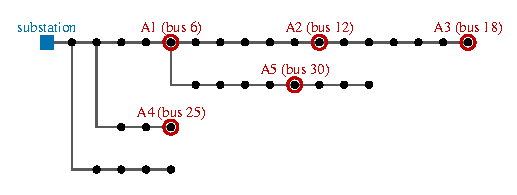
\includegraphics[width=\columnwidth]{generated/fig_feeder_ieee33.pdf}
\caption{IEEE 33-bus feeder (MATPOWER data, open ties removed) with the five
aggregator connection points A1--A5.}
\label{fig:feeder}
\end{figure}

\subsection{Data}
\emph{Prices.} Hourly Netherlands day-ahead prices from the ENTSO-E
Transparency Platform~\cite{hirth2018}, as distributed with
EV2Gym~\cite{orfanoudakis2025ev2gym}, converted to local standard time:
2023 for training, 2024 for testing, and 2019 as an alternative price regime.

\emph{Household load.} One year of 15-min consumption of 25 Pecan Street
homes~\cite{pecanstreet}, as distributed with EV2Gym~\cite{orfanoudakis2025ev2gym},
averaged and normalized by its 99.5th percentile. The profile scales the
nominal feeder loads, matched by day of year (so training and test days share
it), with multiplicative noise of standard deviation 0.02 at every power-flow
step. The base-load scale is calibrated as the largest value (in steps of
0.01) for which the feeder \emph{without} EVs stays at or above $0.955\pu$ over
the whole year (\GScaleIeeeThreeThree{} for the 33-bus and
\GScaleIeeeSixNine{} for the 69-bus feeder). The voltage problems studied here
are therefore caused by EV charging.

\emph{Vehicles.} The main experiments use a synthetic residential fleet whose
parameters are stated assumptions: arrivals $\mathcal{N}(18,2^2)$\,h clipped to
12:00--23:30, dwell $\mathcal{N}(12,3^2)$\,h clipped to 2--16\,h, initial and
target state of charge $\mathcal{N}(0.35,0.15^2)$ and $\mathcal{N}(0.85,0.10^2)$
(clipped to $[0.05,0.9]$ and to at least $0.05$ above the initial value),
batteries of 40, 60, 75 or \SI{100}{kWh} (equally likely), and chargers of
rating $\bar c=\SI{11}{kW}$ with efficiency $\eta=0.95$. Episodes
run 24\,h from 12:00. For generalization we also use real sessions from
ACN-Data~\cite{lee2019acn} at Caltech and JPL (bundled with
SustainGym~\cite{yeh2023sustaingym}): each sampled vehicle keeps a recorded
session's arrival time, dwell and delivered energy (2019 for training,
2020--2021 for testing, weekdays, episodes from 06:00). Departures are
truncated at the end of the episode and requests capped at what the charger can
deliver during the dwell, so full service is attainable except for the wait
(under \SI{15}{min}) for the first dispatch after arrival. EV penetration is
the number of vehicles per household, with 300 households behind the five
aggregators.

\subsection{Driver Response}
Price response is part of the environment, not a control level. Each vehicle
accepts the execution price $p_k$ of its aggregator with the Fishbein--Ajzen
attitude model~\cite{fishbein1975},
\begin{equation}
P^{\mathrm{acc}}_i=\sigma\!\left(w^{\mathrm{c}}_i\frac{\lambda^{\mathrm{ref}}-p_k}{\lambda^{\mathrm{ref}}}+w^{\mathrm{n}}_i\bar A+b_i\right),
\label{eq:fishbein}
\end{equation}
with logistic $\sigma$, reference rate $\lambda^{\mathrm{ref}}=\text{\euro}0.20/\mathrm{kWh}$,
last-interval fleet acceptance $\bar A$ (floored at 0.3) and heterogeneous
weights $w^{\mathrm{c}}_i\sim\mathcal{N}(5,1)$, $w^{\mathrm{n}}_i\sim\mathcal{N}(2,0.5^2)$,
$b_i\sim\mathcal{N}(0,0.5^2)$. A driver whose remaining need exceeds 0.7 times
the charger rating times the hours to departure accepts regardless of price.
Acceptance is drawn once per dispatch interval.

\subsection{Energy Accounting and Metrics}
\label{sec:metrics}
A vehicle draws power only while it is plugged in, has accepted the current
price and still needs energy, and it never draws more than completes its need
within a step. The energy cost is the day-ahead price times the energy
actually drawn (after any curtailment). We report the daily cost (\euro), the
cost per delivered kWh, the service quality (SQ, delivered over requested
energy), the violation rate (Viol., share of 60-s steps with any bus
below $\vlim=0.95\pu$ after any correction), the mean daily minimum voltage
(the lowest bus voltage $V^{\min}$ of each day, averaged over days; in
general, $V^{\min}$ is the lowest bus voltage of the period considered), the
curtailed energy (Curt.) and the unmet energy (need left when vehicles depart),
both in kWh per day, and the mean retail price paid by drivers (Retail).

\section{Nested Controller}
\label{sec:method}
Fig.~\ref{fig:arch} shows the architecture. Each level is a decision process
at its own rate whose environment includes the drivers' price response and
the closed-loop behavior of the faster levels.

\begin{figure*}[t]
\centering
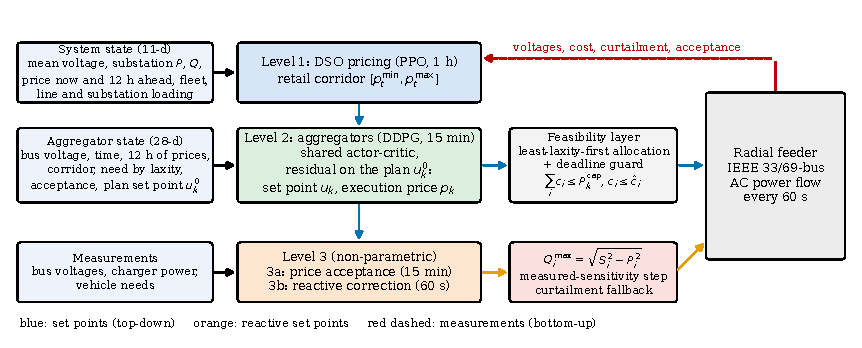
\includegraphics[width=\textwidth]{generated/fig_architecture.pdf}
\caption{Nested controller. Black arrows: observations; blue: set points
(top-down); orange: reactive set points computed by Level~3 from measured
voltages; red, dashed: measurements fed back (bottom-up).}
\label{fig:arch}
\end{figure*}

\subsection{Level 1: Price Corridor (PPO, Hourly)}
The state $s^{(1)}_t\in\mathbb{R}^{11}$ holds the mean bus voltage, the
substation active and reactive power, the current day-ahead price, the share of
vehicles plugged in, their mean state of charge, the line-loading margin
(assumed rating \SI{0.4}{kA} per line), the substation loading (assumed
\SI{8}{MVA}), the hour (sine and cosine) and the mean price over the next
12\,h. The action $a^{(1)}_t\in[0,1]^2$, drawn from Beta distributions, sets
the center $c_t$ and width $w_t$ of the corridor
$[p^{\min}_t,p^{\max}_t]=[c_t-w_t/2,\,c_t+w_t/2]$ (clipped to
$[p^{\mathrm{lo}},p^{\mathrm{hi}}]$):
\begin{align}
c_t&=\lambda^{\mathrm{ref}}+(2a^{(1)}_{t,1}-1)\begin{cases}\lambda^{\mathrm{ref}}-p^{\mathrm{lo}}, & a^{(1)}_{t,1}<0.5,\\ p^{\mathrm{hi}}-\lambda^{\mathrm{ref}}, & \text{otherwise,}\end{cases}\nonumber\\
w_t&=w^{\min}+a^{(1)}_{t,2}\,(w^{\max}-w^{\min}),
\label{eq:corridor}
\end{align}
with bounds $p^{\mathrm{lo}}=\text{\euro}0.05$ and $p^{\mathrm{hi}}=\text{\euro}0.40/\mathrm{kWh}$
and widths $w^{\min}=\text{\euro}0.02$ and $w^{\max}=\text{\euro}0.20/\mathrm{kWh}$.
The neutral action $(0.5,0.5)$ gives the \emph{neutral corridor}
$[\text{\euro}\GNeutralLo,\text{\euro}\GNeutralHi]/\mathrm{kWh}$, centered on
the reference rate, so an untrained policy, whose mean action is close to it,
charges about the flat tariff of the baselines. The reward of hour $t$,
\begin{align}
r^{(1)}_t={}&-\frac{C_t}{100}-50\,(20\,\Delta V_t)^2-10\,\mathbb{I}[\Delta V_t>0]\nonumber\\
&-5\,\frac{U_t}{100}-0.5\,\frac{X_t}{100}+\omega\,\frac{R_t-\lambda^{\mathrm{ref}}E^{\mathrm{del}}_t}{100},
\label{eq:r1}
\end{align}
penalizes energy cost $C_t$, the voltage deficit $\Delta V_t=\max(0,\vlim-V^{\min}_t)$
with $V^{\min}_t$ the lowest bus voltage of the hour, unmet energy $U_t$ of
departing vehicles and curtailment $X_t$ ($\mathbb{I}$: indicator); the last
term, with retail revenue $R_t$ and delivered energy $E^{\mathrm{del}}_t$, is the
revenue-neutrality term defined below. PPO~\cite{schulman2017} trains the
policy with clipping 0.2, $\gamma=0.99$ and generalized advantage estimation
(GAE) with $\lambda_{\mathrm{GAE}}=0.95$.

\subsection{Level 2: Plan-Residual Dispatch (DDPG, 15 min)}
\emph{State.} The state of aggregator $k$, $s^{(2)}_{\tau,k}\in\mathbb{R}^{28}$,
holds its bus voltage, the hour, the current price, the day-ahead prices of
the current and the next 11 hours, the corridor, the number of plugged-in
vehicles, their remaining energy need (total, and split into four laxity bins:
below 1, 1--3, 3--6 and above 6\,h), the power they can absorb, their mean
remaining dwell, the last fleet acceptance rate, and the plan set point
$u^0_{\tau,k}$ defined below. One actor $\mu$ and one critic are shared by the
five aggregators, with a one-hot aggregator identifier appended to the state
(parameter sharing~\cite{gupta2017}).

\emph{Planning prior.} For each plugged-in vehicle $i$ with remaining need
$e_i$, the plan selects the $\lceil e_i/(\eta\bar c\Delta)\rceil$ cheapest
intervals before departure ($\Delta=\SI{15}{min}$); prices beyond the 12-h
look-ahead are valued at the mean known price. The plan set point
$u^0_{\tau,k}\in[0,1]$ is the power of the vehicles whose current interval is
selected, as a fraction of the power the aggregator can deliver now. The plan
uses only information the aggregator has: the price look-ahead and the needs
and departure times of its plugged-in vehicles.

\emph{Action.} The actor outputs $a_{\tau,k}=\mu(s^{(2)}_{\tau,k})\in[0,1]^2$.
The first component corrects the plan, and the second sets the execution price
inside the corridor:
\begin{align}
u_{\tau,k}&=\mathrm{clip}\big(u^0_{\tau,k}+\rho\,(2a_{\tau,k,1}-1),\,0,\,1\big),
\label{eq:residual}\\
p_{\tau,k}&=p^{\min}_t+a_{\tau,k,2}\,(p^{\max}_t-p^{\min}_t),
\label{eq:price}
\end{align}
so an actor output of $a_{\tau,k,1}=0.5$ reproduces the plan; the residual
scale $\rho$ is listed in Table~\ref{tab:hyper}.

\emph{Feasibility by construction.} Let $\hat c_i=\min\{\bar c,\,e_i/(\eta\Delta)\}$
for the vehicles that accepted the price. The set point dispatches
$P_{\tau,k}=u_{\tau,k}\min\{P^{\mathrm{cap}}_k,\sum_i\hat c_i\}$, which is
filled in order of increasing laxity $\ell_i=h_i-e_i/(\eta\bar c)$ ($h_i$:
hours to departure)~\cite{xu2016priority}. A deadline guard raises $P_{\tau,k}$
to cover every vehicle with $\ell_i\le\Delta$, up to the same limit. Every
dispatch therefore lies in
\begin{equation}
\mathcal{C}_k=\Big\{c:\ 0\le c_i\le\hat c_i,\ \textstyle\sum_i c_i\le P^{\mathrm{cap}}_k\Big\}.
\label{eq:feasible}
\end{equation}
Methods that output per-vehicle rates are mapped onto $\mathcal{C}_k$ by exact
Euclidean projection (bisection on the dual of the sum constraint).

\emph{Reward.} The reward of aggregator $k$ in interval $\tau$ is
\begin{align}
r^{(2)}_{\tau,k}={}&-C_{\tau,k}+\omega\,(p_{\tau,k}-\lambda^{\mathrm{ref}})E^{\mathrm{del}}_{\tau,k}\nonumber\\
&-2\,U_{\tau,k}-0.5\,G_{\tau,k}-0.5\,X_{\tau,k},
\label{eq:r2}
\end{align}
where $C_{\tau,k}$ is the energy cost of the interval (summed over a day it is
exactly the daily cost), $U_{\tau,k}$ the unmet energy of departing vehicles,
$G_{\tau,k}$ the energy that can no longer be delivered before departure and
$X_{\tau,k}$ the curtailed energy (energies in kWh, money in \euro). Because one
day spans 96 decisions, we use $\gamma=0.999$; with $\gamma=0.99$ a cost
incurred 12\,h later would be discounted by almost 40\% ($0.99^{48}\approx0.62$).

\emph{Revenue-neutral pricing.} A profit-seeking aggregator would raise retail
prices, which lowers acceptance and pushes charging into expensive hours. We
instead require the mean retail price paid to equal the flat reference rate
$\lambda^{\mathrm{ref}}$ charged by the non-pricing baselines. The weight
$\omega$ in~\eqref{eq:r1} and~\eqref{eq:r2} is the Lagrange multiplier of this
constraint. Plain dual ascent oscillated in our experiments, so after every
training episode we use a proportional--integral (PI) Lagrangian
update~\cite{stooke2020pid},
\begin{align}
\varepsilon&=(\lambda^{\mathrm{ref}}-\bar p)/\lambda^{\mathrm{ref}},\qquad \bar\varepsilon\leftarrow(1-\alpha)\,\bar\varepsilon+\alpha\,\varepsilon,\nonumber\\
\omega&=\mathrm{clip}\Big(K_p\,\bar\varepsilon+K_i\textstyle\sum\varepsilon,\ \omega^{\min},\ \omega^{\max}\Big),
\label{eq:dual}
\end{align}
where $\bar p$ is the mean retail price paid in the episode, $\bar\varepsilon$
is an exponential moving average (EMA) with weight $\alpha$, and the sum runs
over past episodes and is clipped against wind-up (gains and bounds in
Table~\ref{tab:hyper}). The multiplier enforces the constraint on average over
the training episodes; the final deterministic policy can still charge
slightly more or less than $\lambda^{\mathrm{ref}}$. After training we
therefore calibrate the tariff level: a constant offset added to every
execution price (the sum clipped to $[p^{\mathrm{lo}},p^{\mathrm{hi}}]$, so it
may leave the corridor by up to the offset) is found by bisection such that,
on ten randomly drawn 2023 training days, the deterministic policy's mean
retail price paid equals $\lambda^{\mathrm{ref}}$. The same calibration is
applied to every learned method, uses only training data and moved prices by
at most \euro\GCalibOffsetAbsmax/kWh. Prices can thus shift charging in time
while drivers pay about the reference rate.

DDPG~\cite{lillicrap2016} trains the actor and critic (256--128--64 units) on
transitions $(s_\tau,a_\tau,r_\tau,s_{\tau+1})$, where $a_\tau$ is the action
\emph{actually applied} after the guard, mapped back
through~\eqref{eq:residual} and clipped to $[0,1]$. The actor's output layer is
initialized near zero, so training starts from the plan.

\subsection{Level 3: Reactive Voltage Correction (60 s)}
Level~3 runs inside every 60-s step (Fig.~\ref{fig:l3}). After the power
flow, if $\min_n|V_n|<\vlim+\delta$ (with $\delta=0.001\pu$), the plugged-in
chargers at aggregator bus $k$ offer the headroom
\begin{equation}
\bar Q_k=\sum_{i\in k}\sqrt{\max\{S_i^2-P_i^2,\,0\}},\qquad S_i=\SI{12}{kVA}.
\label{eq:qcap}
\end{equation}
At the full charging power of \GPCharger\,kW a charger thus still offers
\GQFullPower\,kvar, at $P_i=0$ it offers its full rating, and curtailing
active power \emph{increases} reactive headroom. In our model $S_i$ bounds only
the reactive capability; the 11-kW active-power limit is separate. The
first injection is proportional to the voltage gap, saturates when the lowest
voltage $V^{\min}$ reaches $0.90\pu$, and is weighted toward the most depressed
aggregator buses. Each later iteration measures the sensitivity
$\hat s=\Delta V^{\min}/\Delta Q$ between the last two power-flow solutions
and, if $\Delta Q$ and $\Delta V^{\min}$ are both positive, takes the secant step
\begin{equation}
\Delta Q=1.2\,\big(\vlim+\delta-V^{\min}\big)/\hat s,
\label{eq:secant}
\end{equation}
split across buses by voltage depression and capped by the remaining headroom;
otherwise the proportional step is repeated. If no headroom is left, EV power
is shed in steps of up to 20\% per iteration, most at the most depressed bus,
and the flow is re-solved. The loop stops when $V^{\min}\ge\vlim+\delta$ or when
the iteration limit is reached: eight corrective power flows, raised to twenty
once curtailment has started. Because the sensitivity is measured on
successive AC solutions, the step needs no precomputed network model. Level~3
does not depend on the policy above it; we therefore also evaluate it with
every baseline (``+L3'').

\begin{figure}[t]
\centering
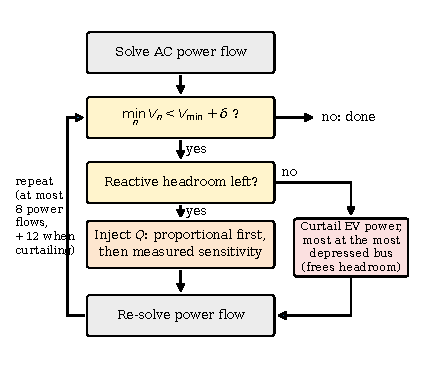
\includegraphics{generated/fig_l3_loop.pdf}
\caption{Level-3 correction inside one 60-s step.}
\label{fig:l3}
\end{figure}

\subsection{Training}
Episodes are random 2023 days. A curriculum raises the fleet from 60 to 300
vehicles in steps of 60 and advances when the last 20 episodes reach mean
SQ $\ge0.95$ with mean curtailment $\le\SI{20}{kWh}$; the final stage draws
the fleet size uniformly between 120 and 300. Each run has
\GTrainEpisodes{} episodes and takes about \GTrainHoursNested~h on a single
CPU core. Algorithm~\ref{alg:main} summarizes one dispatch
interval, and Table~\ref{tab:hyper} lists the hyperparameters, read directly
from the configuration file and the code.

\begin{algorithm}[t]
\caption{One 15-min Interval of the Nested Controller}
\label{alg:main}
\footnotesize
\begin{algorithmic}[1]
\STATE \textbf{if} hour boundary \textbf{then} observe $s^{(1)}$; set corridor by~\eqref{eq:corridor}
\FOR{each aggregator $k$}
  \STATE observe $s^{(2)}_k$ (incl.\ plan $u^0_k$); $a_k\leftarrow\mu(s^{(2)}_k)$
  \STATE set point $u_k$ by~\eqref{eq:residual}; price $p_k$ by~\eqref{eq:price}
\ENDFOR
\STATE drivers accept or decline by~\eqref{eq:fishbein} (environment)
\STATE LLF allocation with deadline guard onto $\mathcal{C}_k$~\eqref{eq:feasible}
\FOR{each of the fifteen 60-s steps}
  \STATE solve the AC power flow~\eqref{eq:pf}
  \STATE \textbf{if} $V^{\min}<\vlim+\delta$ \textbf{then} Level-3 loop~\eqref{eq:qcap}, \eqref{eq:secant}
  \STATE book drawn energy, cost and curtailment
\ENDFOR
\STATE (training) store $(s,a^{\mathrm{applied}},r,s')$; update the DDPG agent
\STATE (training, end of day) update the PPO policy and $\omega$ by~\eqref{eq:dual}
\end{algorithmic}
\end{algorithm}

\begin{table}[t]
\centering
\caption{Hyperparameters, Read From the Configuration File and the Code}
\label{tab:hyper}
\footnotesize
\begin{tabular}{@{}l>{\raggedright\arraybackslash}p{0.68\columnwidth}@{}}
\toprule
Level 1 (PPO) & actor/critic 256--128--64, Beta policy, lr 0.0003, $\gamma$ 0.99, $\lambda_{\mathrm{GAE}}$ 0.95, clip 0.2, 10 epochs per update, entropy 0.001 \\
Level 2 (DDPG) & actor/critic 256--128--64, shared, one-hot id \\
 & lr actor/critic 0.0001/0.001, $\gamma$ 0.999, $\tau$ 0.005 \\
 & batch 128, buffer 200\,000, warm-up 1\,000 transitions \\
 & Gaussian action noise, std 0.3$\to$0.05 (factor 0.995 per episode); residual scale $\rho$ 0.1 \\
Multiplier & $K_p$ 2.0, $K_i$ 0.05, EMA weight $\alpha$ 0.2, $\omega\in[-2.0, 2.0]$, $|K_i\textstyle\sum e|\le2.0$ \\
Training & 600 episodes; curriculum window 20 \\
Baselines & same networks, learning rates, episodes and curriculum; safe RL: $\gamma$ 0.999, cost limit 0, dual step 0.05 (PPO-Lag.), KL radius 0.01 (CPO) \\
Level 3 & $\delta$ 0.001 p.u., $S_i$ 12.0 kVA, $\le$8 (+12 when curtailing) power flows \\
\bottomrule
\end{tabular}

\end{table}

\section{Experimental Setup}
\label{sec:setup}

\subsection{Scenarios}
S1, S2, S3 and S5 use 120, 200, 240 and 300 vehicles (40\%--100\%
penetration). S4 repeats S3 with an hourly-persistent deviation of the base
load from its profile (standard deviation 15\%, clipped to $\pm40\%$); it is a
forecast error for the LP-OPF, the only method that uses a load forecast. Two
stress tests probe Level~3. S6 forbids all charging between 19:00 and 20:00,
so that charging resumes in a synchronized rebound. S7 has 360 vehicles
(120\%) and emulates reduced reactive capability by halving the inverter
rating to $S_i=\GSRatedSSeven$\,kVA: a charger drawing more than
\SI{6}{kW} then offers no reactive power.

\subsection{Baselines}
\emph{Rule-based.} Uncoordinated charging (full power on arrival); a TOU timer
(off-peak 23:00--07:00, earlier only when laxity is exhausted); and the
price-aware heuristic, which charges each vehicle at full power in its planned
cheapest intervals, that is, the Level-2 plan executed per vehicle, with the
same 12-h price look-ahead.
\emph{Model-predictive LP-OPF.} At every interval an LP over the rest of the
day (HiGHS~\cite{huangfu2018}) minimizes energy cost plus a penalty of
\text{\euro}5/kWh on unmet energy, subject to per-vehicle energy, charger and
transformer limits and to linearized voltage limits ($\ge\vlim+\delta$ at every
bus) from finite-difference sensitivities of the AC power flow at the forecast
base-load (no-EV) operating point of each interval. It has \emph{perfect
foresight} of prices and of every vehicle's arrival, departure and need, which
the asterisk in LP-OPF$^\ast$ marks in tables and figures. It is a strong
model-based reference rather than a deployable controller; it is not a strict
bound, because its voltage model is linearized and drivers may still decline.
\emph{Learned.} Flat DDPG (one agent, all aggregators' states and actions),
PPO-Lagrangian and CPO~\cite{achiam2017} (expected-cost constraint on
violations, limit $d=0$), and a goal-conditioned HRL agent (hourly DDPG goals,
15-min DDPG workers). They observe the same states, including the plan
set point, use the same allocation layer, reward terms, discount factor and
revenue-neutral multiplier, and set execution prices inside the neutral
corridor. Because they are trained without Level~3, Flat DDPG and the HRL agent
add a voltage penalty to the reward (the hierarchical workers also receive a
goal-tracking term), and PPO-Lagrangian and CPO constrain it as the cost. Each
is also evaluated with Level~3 attached. Uncoordinated charging, the
price-aware heuristic and the LP-OPF charge the flat reference rate
$\lambda^{\mathrm{ref}}$; the TOU timer charges its three-tier tariff
(\text{\euro}0.12/kWh 23:00--07:00, \text{\euro}0.30/kWh 17:00--21:00 and
\text{\euro}0.20/kWh otherwise).

\subsection{Protocol}
All methods are evaluated on the same \GEvalDays{} distinct 2024 days, with
identical fleets and noise for each day (paired design). Learned methods are
trained with \GTrainSeedsWord{} seeds (\GAuxSeedsWord{} in the ablations and
generalization tests); each day's metric is averaged over seeds.
We report means with 95\% bootstrap confidence intervals over days (10\,000
resamples) and compare methods with Wilcoxon signed-rank tests on the paired
daily differences, Holm-corrected across the comparison family. The allocation
rule was selected before testing, on \GTuneValDays{} held-out 2023 days with a
criterion fixed in advance: over three variants that serve planned slots
first (\GTuneSeedsWord{} seeds each), the S3 cost fell by up to
\GTuneCostReductionMax\%,% claim: tune_plan_cheaper_S3
\ but \GTuneUnmetIncreaseMinSThree\%--\GTuneUnmetIncreaseMaxSThree\% (S3) and
\GTuneUnmetIncreaseMinSSeven\%--\GTuneUnmetIncreaseMaxSSeven\% (S7) more energy
was left undelivered,% claim: tune_plan_more_unmet
\ so least-laxity-first allocation was kept.% claim: tune_llf_selected

\section{Results}
\label{sec:results}

% Results. Every number is a macro from generated/numbers.tex; every
% qualitative statement tagged "% claim: <name>" is checked against
% generated/claims.json by scripts/check_paper.py.

\begin{table*}[t]
\centering
\caption{Results at S3 (240 vehicles, 80\% penetration; IEEE 33-bus; \GEvalDays{} held-out days; learned methods averaged over \GTrainSeeds{} training seeds). Cost is the daily energy cost with its 95\% bootstrap confidence interval; Retail is the mean retail price paid (\euro/kWh); SQ is the delivered share of requested energy. ``+L3'' attaches the Level-3 layer to a baseline.}
\label{tab:main}
\footnotesize
\begin{tabular}{@{}lrrrrrrr@{}}
\toprule
Method & Cost (\euro) & Cost/kWh & Retail & SQ & Viol.\ (\%) & Mean $V^{\min}$ & Curt.\ (kWh) \\
\midrule
Uncoordinated & 931.4 {\scriptsize[833.8, 1060.7]} & 0.1146 & 0.200 & 1.000 & 3.99 & 0.9554 & 0.0 \\
Uncoordinated + L3 & 931.4 {\scriptsize[835.0, 1062.6]} & 0.1146 & 0.200 & 1.000 & 0.00 & 0.9615 & 5.0 \\
TOU timer & 697.7 {\scriptsize[639.6, 751.2]} & 0.0863 & 0.132 & 0.995 & 4.30 & 0.9372 & 0.0 \\
TOU timer + L3 & 697.1 {\scriptsize[641.0, 750.9]} & 0.0862 & 0.132 & 0.995 & 0.00 & 0.9515 & 23.7 \\
Price-aware heuristic & 619.8 {\scriptsize[561.8, 674.2]} & 0.0766 & 0.200 & 0.997 & 0.73 & 0.9598 & 0.0 \\
Price-aware heuristic + L3 & 619.8 {\scriptsize[564.4, 675.0]} & 0.0766 & 0.200 & 0.997 & 0.00 & 0.9623 & 1.7 \\
MPC LP-OPF (perfect foresight) & 612.0 {\scriptsize[555.7, 667.2]} & 0.0759 & 0.200 & 0.992 & 0.01 & 0.9634 & 0.0 \\
MPC LP-OPF (perfect foresight) + L3 & 612.0 {\scriptsize[555.3, 667.3]} & 0.0759 & 0.200 & 0.992 & 0.00 & 0.9635 & 0.0 \\
\midrule
Flat DDPG & 756.1 {\scriptsize[695.5, 828.3]} & 0.0934 & 0.203 & 0.996 & 0.45 & 0.9673 & 0.0 \\
Flat DDPG + L3 & 756.1 {\scriptsize[694.6, 827.0]} & 0.0934 & 0.203 & 0.996 & 0.00 & 0.9686 & 0.1 \\
PPO-Lagrangian & 790.2 {\scriptsize[725.8, 866.6]} & 0.0976 & 0.199 & 0.996 & 0.19 & 0.9758 & 0.0 \\
PPO-Lagrangian + L3 & 790.2 {\scriptsize[725.2, 865.0]} & 0.0976 & 0.199 & 0.996 & 0.00 & 0.9763 & 0.0 \\
CPO & 816.9 {\scriptsize[747.5, 900.1]} & 0.1006 & 0.200 & 0.999 & 0.35 & 0.9731 & 0.0 \\
CPO + L3 & 817.0 {\scriptsize[748.1, 903.3]} & 0.1006 & 0.200 & 0.999 & 0.00 & 0.9739 & 0.0 \\
Hierarchical RL & 741.3 {\scriptsize[685.3, 799.4]} & 0.0915 & 0.200 & 0.997 & 0.03 & 0.9741 & 0.0 \\
Hierarchical RL + L3 & 741.3 {\scriptsize[685.3, 800.0]} & 0.0915 & 0.200 & 0.997 & 0.00 & 0.9743 & 0.0 \\
\midrule
Nested (proposed) & 645.0 {\scriptsize[590.0, 700.0]} & 0.0797 & 0.201 & 0.997 & 0.00 & 0.9665 & 0.4 \\
\bottomrule
\end{tabular}

\end{table*}

\subsection{Main comparison}
\label{sec:res-main}
Table~\ref{tab:main} compares all methods at S3. Uncoordinated charging costs
\GUncoordinatedSThreeCost~\euro{} per day and violates the voltage floor in
\GUncoordinatedSThreeViol\% of the \SI{60}{s} steps.% claim: unc_violates_main
\ Attaching Level~3 removes every violation of the rule-based methods at
S1, S2, S3 and S5% claim: l3_zero_viol_rules_nominal
\ without changing their cost, because the correction uses reactive power and
curtails only when the headroom is exhausted. The perfect-foresight LP-OPF is
the cheapest method (\GLpOpfLThreeSThreeCost~\euro).% claim: lp_cheapest_S3
\ Among the methods that do not see the future, the price-aware heuristic is
cheapest (\GPriceAwareLThreeSThreeCost~\euro).% claim: pa_cheapest_nonoracle_S3
\ The nested controller costs \GNestedSThreeCost~\euro, which is
\GSavingNestedUncSThree\% less than uncoordinated charging and
\GGapNestedPaSThree\% more than the price-aware heuristic,% claim: pa_cheaper_than_nested_all_main
\ with no violations,% claim: nested_zero_viol_nominal
\ a service quality of \GNestedSThreeSq{} and a mean retail price of
\GNestedSThreeRetail~\euro/kWh. It is the cheapest learned controller,
\GSavingNestedBestLearnedSThree\% below the best learned baseline
(\GBestLearnedSThree).% claim: nested_cheapest_learned_main


\begin{table*}[t]
\centering
\caption{Daily energy cost (\euro) and violation rate (\%) across penetration levels S1--S5 (S4: S3 with \SI{15}{\percent} load-forecast error).}
\label{tab:scenarios}
\footnotesize
\begin{tabular}{@{}lrrrrrrrrrr@{}}
\toprule
Method & \multicolumn{2}{c}{S1 (40\%)} & \multicolumn{2}{c}{S2 (67\%)} & \multicolumn{2}{c}{S3 (80\%)} & \multicolumn{2}{c}{S4 (80\%)} & \multicolumn{2}{c}{S5 (100\%)} \\
 & Cost & Viol. & Cost & Viol. & Cost & Viol. & Cost & Viol. & Cost & Viol. \\
\midrule
Uncoordinated & 474 & 0.42 & 780 & 2.35 & 931 & 3.99 & 931 & 4.53 & 1161 & 6.82 \\
TOU timer & 358 & 0.06 & 587 & 2.39 & 698 & 4.30 & 695 & 4.31 & 858 & 7.55 \\
Uncoordinated + L3 & 474 & 0.00 & 780 & 0.00 & 931 & 0.00 & 931 & 0.02 & 1161 & 0.00 \\
TOU timer + L3 & 358 & 0.00 & 587 & 0.00 & 697 & 0.00 & 695 & 0.00 & 858 & 0.00 \\
Price-aware heuristic + L3 & 317 & 0.00 & 520 & 0.00 & 620 & 0.00 & 618 & 0.02 & 773 & 0.00 \\
MPC LP-OPF (perfect foresight) + L3 & 313 & 0.00 & 513 & 0.00 & 612 & 0.00 & 610 & 0.00 & 765 & 0.00 \\
Flat DDPG & 409 & 0.09 & 642 & 0.30 & 756 & 0.45 & 754 & 0.84 & 931 & 1.11 \\
PPO-Lagrangian & 403 & 0.01 & 662 & 0.16 & 790 & 0.19 & 788 & 0.62 & 984 & 0.51 \\
CPO & 420 & 0.03 & 684 & 0.27 & 817 & 0.35 & 814 & 0.93 & 1016 & 0.81 \\
Hierarchical RL & 380 & 0.00 & 622 & 0.04 & 741 & 0.03 & 739 & 0.38 & 922 & 0.19 \\
Nested (proposed) & 329 & 0.00 & 540 & 0.00 & 645 & 0.00 & 642 & 0.00 & 806 & 0.00 \\
\bottomrule
\end{tabular}

\end{table*}

\begin{figure*}[t]
\centering
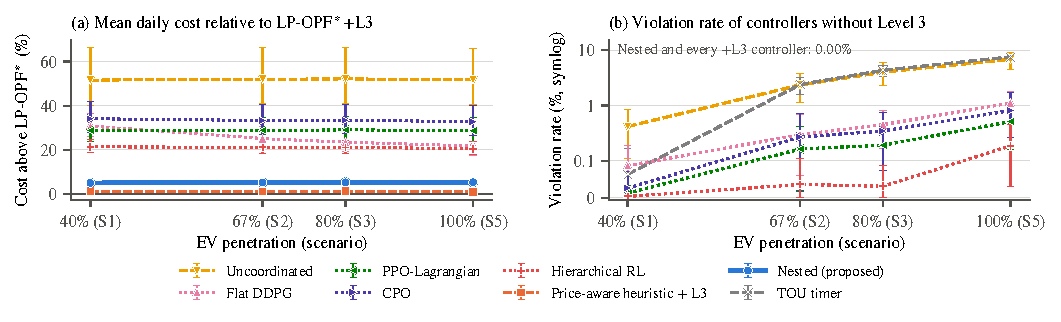
\includegraphics[width=\textwidth]{generated/fig_scenarios.pdf}
\caption{Cost per delivered kWh, service quality and violation rate across S1--S5 (means with 95\% bootstrap confidence intervals over days).}
\label{fig:scenarios}
\end{figure*}

\subsection{Penetration and forecast error}
\label{sec:res-scen}
Table~\ref{tab:scenarios} and Fig.~\ref{fig:scenarios} extend the comparison
to S1--S5. Without Level~3, violations of uncoordinated and TOU charging
grow with penetration, up to \GViolUncMax\% and \GViolTouMax\%.% claim: tou_violates_main
\ With accurate load forecasts (S1, S2, S3, S5) the nested controller and
every ``+L3'' method record no violations.% claim: nested_zero_viol_nominal
% claim: l3_zero_viol_rules_nominal
% claim: l3_zero_viol_learned_nominal
\ S4 is different: with a \SI{15}{\percent} base-load forecast error, the
household load alone breaks the floor on \GNoevViolDaysSFour{} of the
\GEvalDays{} days even when no vehicle charges. Level~3 removes most of these
violations with the reactive headroom of idle chargers ($\Qmax_i=S_i$ at
$P_i=0$); the remainder, at most \GViolNestedMaxSFour\% of the steps for the
nested controller, occurs only on those days.% claim: s4_l3_violations_only_base_load_days
\ The ordering of costs is the same at every penetration level: the nested
controller saves \GSavingNestedUncMin--\GSavingNestedUncMax\% relative to
uncoordinated charging, costs \GGapNestedPaMin--\GGapNestedPaMax\% more than the
price-aware heuristic, and stays below every learned baseline by at least
\GSavingNestedBestLearnedMin\%.% claim: nested_cheapest_learned_main


\begin{table}[t]
\centering
\caption{Paired comparison at S3: daily differences (nested minus method) with 95\% bootstrap intervals and Holm-corrected Wilcoxon signed-rank $p$-values.}
\label{tab:stats}
\footnotesize
\setlength{\tabcolsep}{3pt}
\begin{tabular}{@{}lrrrrr@{}}
\toprule
Nested vs. & $\Delta$Cost (\euro) & $p_{\mathrm{Holm}}$ & Days & $\Delta$SQ & $p_{\mathrm{Holm}}$ \\
\midrule
Uncoord. & -285.7 {\scriptsize[-376.8, -218.8]} & $<\!0.001$ & 50/50 & -0.0028 & $<\!0.001$ \\
Uncoord.+L3 & -285.7 {\scriptsize[-375.4, -219.4]} & $<\!0.001$ & 50/50 & -0.0028 & $<\!0.001$ \\
TOU & -52.0 {\scriptsize[-73.2, -32.7]} & $<\!0.001$ & 40/50 & +0.0014 & 0.070 \\
TOU+L3 & -51.3 {\scriptsize[-72.2, -32.4]} & $<\!0.001$ & 40/50 & +0.0016 & 0.019 \\
Price-aware & +25.9 {\scriptsize[+22.5, +29.8]} & $<\!0.001$ & 0/50 & +0.0001 & 1.000 \\
Price-aware+L3 & +25.9 {\scriptsize[+22.5, +29.8]} & $<\!0.001$ & 0/50 & +0.0001 & 1.000 \\
LP-OPF$^\ast$ & +33.7 {\scriptsize[+29.6, +38.5]} & $<\!0.001$ & 0/50 & +0.0046 & $<\!0.001$ \\
LP-OPF$^\ast$+L3 & +33.7 {\scriptsize[+29.6, +38.3]} & $<\!0.001$ & 0/50 & +0.0046 & $<\!0.001$ \\
Flat DDPG & -125.6 {\scriptsize[-157.5, -103.2]} & $<\!0.001$ & 50/50 & +0.0004 & 0.015 \\
Flat DDPG+L3 & -125.6 {\scriptsize[-157.4, -103.5]} & $<\!0.001$ & 50/50 & +0.0004 & 0.015 \\
PPO-Lag. & -151.4 {\scriptsize[-185.4, -124.8]} & $<\!0.001$ & 50/50 & +0.0009 & $<\!0.001$ \\
PPO-Lag.+L3 & -151.4 {\scriptsize[-185.8, -124.8]} & $<\!0.001$ & 50/50 & +0.0009 & $<\!0.001$ \\
CPO & -167.6 {\scriptsize[-212.3, -134.2]} & $<\!0.001$ & 50/50 & -0.0016 & $<\!0.001$ \\
CPO+L3 & -167.7 {\scriptsize[-211.2, -135.0]} & $<\!0.001$ & 50/50 & -0.0016 & $<\!0.001$ \\
HRL & -96.0 {\scriptsize[-106.7, -85.7]} & $<\!0.001$ & 50/50 & -0.0001 & 1.000 \\
HRL+L3 & -96.0 {\scriptsize[-106.9, -86.0]} & $<\!0.001$ & 50/50 & -0.0001 & 1.000 \\
\bottomrule
\end{tabular}

\end{table}

\subsection{Statistical comparison}
\label{sec:res-stats}
Table~\ref{tab:stats} tests the daily differences at S3. The cost differences
to uncoordinated charging and to every learned baseline are significant after
Holm correction,% claim: nested_sig_cheaper_all_learned_S3
\ and so is the cost premium relative to the price-aware heuristic% claim: nested_sig_costlier_than_price_aware_L3_S3
\ and the LP-OPF.% claim: nested_sig_costlier_than_lp_opf_L3_S3
\ The ``Days'' column counts the days on which the nested controller is the
cheaper of the pair.


\begin{table}[t]
\centering
\caption{Level-3 stress tests. S6 forbids charging from 19:00 to 20:00; S7 has 360 vehicles with inverters derated to 50\%. Violation rate (\%), minimum voltage (p.u.), curtailed and unmet energy (kWh per day) and service quality.}
\label{tab:stress}
\footnotesize
\setlength{\tabcolsep}{2pt}
\begin{tabular}{@{}lrrrrrr@{}}
\toprule
Method & \multicolumn{2}{c}{S6} & \multicolumn{4}{c}{S7} \\
\cmidrule(lr){2-3}\cmidrule(lr){4-7}
 & Viol. & $V_{\min}$ & Viol. & Curt. & Unmet & SQ \\
\midrule
Uncoord. & 3.80 & 0.951 & 9.00 & 0 & 6 & 1.000 \\
TOU & 4.32 & 0.937 & 10.62 & 0 & 402 & 0.968 \\
Uncoord.+L3 & 0.00 & 0.958 & 0.35 & 492 & 15 & 0.999 \\
TOU+L3 & 0.00 & 0.951 & 0.17 & 682 & 561 & 0.955 \\
Price-aware+L3 & 0.00 & 0.962 & 0.16 & 139 & 106 & 0.991 \\
LP-OPF$^\ast$+L3 & 0.00 & 0.963 & 0.00 & 0 & 98 & 0.992 \\
Nested & 0.00 & 0.966 & 0.01 & 46 & 38 & 0.997 \\
\bottomrule
\end{tabular}

\end{table}

\subsection{Level 3 under stress}
\label{sec:res-stress}
Table~\ref{tab:stress} probes Level~3 beyond nominal conditions. In S6 no
charging is allowed for an hour in the evening peak; because reactive headroom
is bounded by the inverter rating rather than by charging power, every
controller with Level~3 keeps the floor. S7 exceeds what halved inverters can
correct, and the methods separate. The nested controller curtails
\GReductionCurtNestedPaSSeven\% less energy than the price-aware heuristic,% claim: nested_less_curtailment_than_pa_S7
\ leaves \GReductionUnmetNestedPaSSeven\% less energy undelivered% claim: nested_less_unmet_than_pa_S7
\ and has \GReductionViolNestedPaSSeven\% fewer violations;% claim: nested_fewer_viol_than_pa_S7
\ its service quality is \GNestedSSevenSq{} against
\GPriceAwareLThreeSSevenSq.% claim: nested_higher_sq_than_pa_S7
\ The price of this robustness is energy cost: \GNestedSSevenCost~\euro{}
against \GPriceAwareLThreeSSevenCost~\euro{} per day.% claim: pa_cheaper_than_nested_S7


\begin{table}[t]
\centering
\caption{What the learned levels add (Level~3 active throughout). Plan: the Level-2 planning prior executed without learning; Prices only: learned corridor and execution prices with plan dispatch; Dispatch only: learned residual dispatch at the flat tariff. Daily cost (\euro), retail price (\euro/kWh), violations (\%), curtailed and unmet energy (kWh per day).}
\label{tab:decomp}
\footnotesize
\setlength{\tabcolsep}{2pt}
\begin{tabular}{@{}lrrrrrrr@{}}
\toprule
 & \multicolumn{3}{c}{S3} & \multicolumn{4}{c}{S7} \\
\cmidrule(lr){2-4}\cmidrule(lr){5-8}
Configuration & Cost & Retail & SQ & Cost & Viol. & Curt. & Unmet \\
\midrule
Price-aware+L3 & 619.8 & 0.200 & 0.997 & 940.4 & 0.16 & 139 & 106 \\
Plan+L3 & 627.9 & 0.200 & 0.997 & 956.7 & 0.02 & 114 & 37 \\
Prices only & 633.9 & 0.201 & 0.997 & 966.3 & 0.03 & 82 & 43 \\
Dispatch only & 645.3 & 0.200 & 0.998 & 981.4 & 0.03 & 71 & 30 \\
Nested & 645.0 & 0.201 & 0.997 & 982.9 & 0.01 & 46 & 38 \\
\bottomrule
\end{tabular}

\end{table}

\subsection{What the learned levels add}
\label{sec:res-decomp}
Table~\ref{tab:decomp} separates what each learned level contributes, with
Level~3 active throughout. Executed without learning, the plan costs
\GDecompCostVsPlanAbsPriceAwareLThreeSThree\% more at S3 than the per-vehicle
price-aware heuristic,% claim: decomp_price_aware_L3_cheaper_than_plan_S3
\ because the aggregate set point is filled least-laxity-first rather than by
each vehicle's own cheapest slots. Relative to the plan, learned prices alone
raise the S3 cost by \GDecompCostVsPlanAbsNestedPlanpriceSThree\%,% claim: decomp_nested_planprice_costlier_than_plan_S3
\ learned dispatch alone by \GDecompCostVsPlanAbsNestedFlatpriceSThree\%,% claim: decomp_nested_flatprice_costlier_than_plan_S3
\ and the full controller by \GDecompCostVsPlanAbsNestedSThree\%.% claim: decomp_nested_costlier_than_plan_S3
\ The learned dispatch spreads load away from the cheapest slots, which costs
energy at nominal load but pays off when the feeder is stressed: in S7 it
curtails \GDecompCurtVsPlanNestedFlatpriceSSeven\% less energy than the
plan% claim: decomp_nested_flatprice_less_curt_than_plan_S7
\ and leaves \GDecompUnmetVsPlanNestedFlatpriceSSeven\% less energy
undelivered.% claim: decomp_nested_flatprice_less_unmet_than_plan_S7

\begin{table}[t]
\centering
\caption{Ablations at S3 and S5 (daily cost in \euro, SQ, violation rate in \%).}
\label{tab:ablation}
\footnotesize
\setlength{\tabcolsep}{2.5pt}
\begin{tabular}{@{}lrrrrrr@{}}
\toprule
Configuration & \multicolumn{3}{c}{S3} & \multicolumn{3}{c}{S5} \\
 & Cost & SQ & Viol. & Cost & SQ & Viol. \\
\midrule
Complete framework & 645.7 & 0.997 & 0.00 & 806.6 & 0.997 & 0.00 \\
No planning prior & 696.5 & 0.996 & 0.00 & 865.5 & 0.996 & 0.00 \\
No Level 1 & 642.8 & 0.996 & 0.00 & 804.6 & 0.996 & 0.00 \\
Single timescale & 651.2 & 0.996 & 0.00 & 812.8 & 0.996 & 0.00 \\
No behavior model & 639.4 & 1.000 & 0.00 & 800.0 & 0.999 & 0.00 \\
No Level 3 (trained) & 648.5 & 0.996 & 0.23 & 810.5 & 0.995 & 0.71 \\
Level 3 removed at test & 645.7 & 0.997 & 0.33 & -- & -- & -- \\
No curriculum & 639.2 & 0.996 & 0.00 & 797.3 & 0.996 & 0.00 \\
No deadline guard & 651.2 & 0.996 & 0.00 & 814.6 & 0.996 & 0.00 \\
Proportional allocation & 660.8 & 0.995 & 0.00 & 828.5 & 0.995 & 0.00 \\
\bottomrule
\end{tabular}

\end{table}

\subsection{Ablations}
\label{sec:res-abl}

\begin{table}[t]
\centering
\caption{Generalization at 80\% penetration: second feeder, real ACN-Data sessions and the 2019 price regime (Unc.: uncoordinated; PA: price-aware; LP$^\ast$: perfect-foresight LP-OPF).}
\label{tab:general}
\footnotesize
\setlength{\tabcolsep}{2pt}
\begin{tabular}{@{}lrrrrrrr@{}}
\toprule
 & \multicolumn{4}{c}{Daily cost (\euro)} & \multicolumn{2}{c}{Viol.\ (\%)} & SQ \\
\cmidrule(lr){2-5}\cmidrule(lr){6-7}\cmidrule(lr){8-8}
Setting & Unc. & PA+L3 & LP$^\ast$+L3 & Nested & Unc. & Nested & Nested \\
\midrule
33-bus, residential & 931.4 & 619.8 & 612.0 & 645.0 & 3.99 & 0.00 & 0.997 \\
69-bus, residential & 931.4 & 619.8 & 611.7 & 648.0 & 0.21 & 0.00 & 0.997 \\
33-bus, ACN Caltech & 146.5 & 121.3 & 119.7 & 126.0 & 0.00 & 0.00 & 0.970 \\
33-bus, ACN JPL & 263.8 & 194.1 & 197.1 & 207.0 & 0.00 & 0.00 & 0.994 \\
33-bus, 2019 days & 371.1 & 282.3 & 280.2 & 289.9 & 4.72 & 0.00 & 0.997 \\
\bottomrule
\end{tabular}

\end{table}

\subsection{Generalization}
\label{sec:res-gen}

\begin{table}[t]
\centering
\caption{Sensitivity of Level 3 at S3 (nested controller): correction margin $\delta$ and inverter rating $S_i$ (default $\delta=0.001\pu$, $S_i=\SI{12}{kVA}$).}
\label{tab:sensitivity}
\footnotesize
\setlength{\tabcolsep}{3pt}
\begin{tabular}{@{}lrrrrr@{}}
\toprule
Setting & Cost (\euro) & SQ & Viol.\ (\%) & $Q$ act.\ (\%) & Curt.\ (kWh) \\
\midrule
$\delta = 0.0005$ & 645.7 & 0.997 & 0.000 & 0.36 & 0.5 \\
Default & 645.7 & 0.997 & 0.000 & 0.38 & 0.6 \\
$\delta = 0.002$ & 645.7 & 0.997 & 0.000 & 0.44 & 0.7 \\
$S_i = 10$ kVA & 645.8 & 0.997 & 0.000 & 0.38 & 4.7 \\
$S_i = 14$ kVA & 645.7 & 0.997 & 0.000 & 0.38 & 0.1 \\
\bottomrule
\end{tabular}

\end{table}

\subsection{Level-3 parameters}
\label{sec:res-sens}

\begin{figure*}[t]
\centering
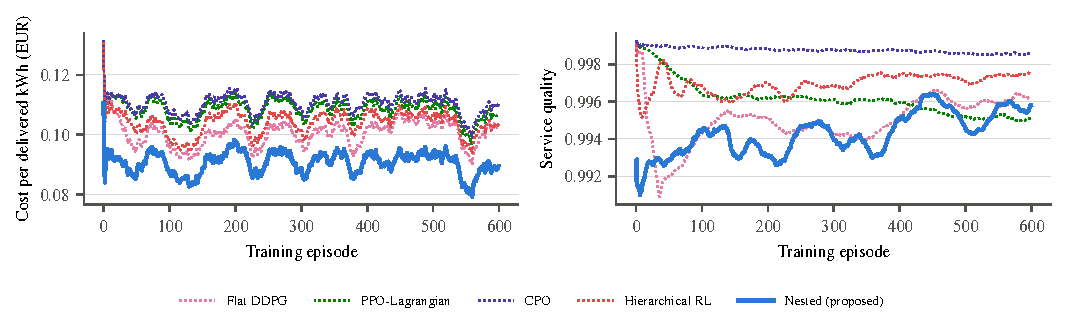
\includegraphics[width=\textwidth]{generated/fig_training.pdf}
\caption{Training curves (rolling mean over 25 episodes, averaged over seeds; exploration noise active).}
\label{fig:training}
\end{figure*}

\begin{table}[t]
\centering
\caption{Training cost on one CPU core per run.}
\label{tab:compute}
\footnotesize
\begin{tabular}{@{}lrrrr@{}}
\toprule
Method & Seeds & Episodes & s / episode & h / run \\
\midrule
CPO & 5 & 600 & 0.43 & 0.07 \\
Flat DDPG & 5 & 600 & 0.81 & 0.14 \\
Hierarchical RL & 5 & 600 & 2.69 & 0.45 \\
Nested (proposed) & 5 & 600 & 2.83 & 0.47 \\
PPO-Lagrangian & 5 & 600 & 0.35 & 0.06 \\
\bottomrule
\end{tabular}

\end{table}

\subsection{Training and computation}
\label{sec:res-comp}


\section{Discussion}
\label{sec:discussion}

\subsection{Role of Learning}
\label{sec:disc-learning}
At nominal load, learning does not lower the energy bill relative to a
well-designed rule: the price-aware heuristic, which executes the Level-2 plan
per vehicle, is cheaper than the nested controller,% claim: pa_cheaper_than_nested_all_main
\ and neither the learned prices nor the learned dispatch reduce cost relative
to the plan (Table~\ref{tab:decomp}).% claim: decomp_nested_planprice_costlier_than_plan_S3
% claim: decomp_nested_flatprice_costlier_than_plan_S3
\ The learned levels reduce curtailment, which mattered under stress
(S7);% claim: decomp_nested_less_curt_than_plan_S7
\ the lower unmet energy under stress comes from least-laxity-first
allocation, not from learning.% claim: plan_less_unmet_than_pa_S7
% claim: decomp_nested_more_unmet_than_plan_S7
\ Learned dispatch needs the plan as a starting point: learned from scratch,
it is costlier at both penetration levels tested (S3 and
S5).% claim: abl_abl_no_prior_costlier_S3
% claim: abl_abl_no_prior_costlier_S5
\ The nested design is therefore not a way to beat optimization on cost but a
way to keep learned components where they help while planning and physics
handle the rest.

\subsection{Scope of the Voltage Correction}
Level~3 is corrective control on the simulated quasi-static state, not an a
priori guarantee. It restores the floor whenever the reactive headroom of the
plugged-in chargers suffices, and otherwise sheds EV power until the floor is
met or the iteration limit is reached (Section~\ref{sec:method}). Three
consequences follow. First, the inverter apparent-power rating sets the
voltage margin: Section~\ref{sec:res-sens} reports the effect of $S_i$, and S7
the behavior when the reactive capability is halved. Second, we assume, as
in~\cite{leemput2015}, that a charger can supply reactive power at any active
power, including when it does not charge; chargers without this capability
offer only the curtailment fallback. Third, the floor is applied at the
medium-voltage (\SI{12.66}{kV}) buses of the test feeders; drops in service transformers and
secondary circuits are not modeled, and the correction acts at the 60-s
resolution of the simulation, so switching transients and sub-cycle dynamics
are outside its scope, as in any quasi-static study.

\subsection{Assumptions and Limitations}
\emph{Information.} The plan, the learned agents and the heuristic know each
plugged-in vehicle's departure time and remaining need, as in managed-charging
programs where drivers enter them~\cite{lee2019acn}. They do not know future
arrivals. Only the LP-OPF reference sees the whole day in advance.
\emph{Network.} The feeders are balanced, radial and single-phase equivalent;
unbalanced three-phase operation can change the voltage sensitivities on which
the correction step relies.
\emph{Behavior.} The acceptance model~\eqref{eq:fishbein} is stylized. The
voltage layer does not depend on it, but the value of price signals does.
\emph{Fleets.} The residential fleet is synthetic with stated parameters; the
ACN experiments use recorded sessions from workplace sites.
\emph{Data.} Household loads (Pecan Street, United States) and day-ahead prices
(Netherlands) come from different systems; they provide realistic daily shapes,
not a model of one particular utility. Training and test days share the
base-load profile and differ in prices, fleets and noise. Adaptation to
structural market change is not tested beyond the 2019 price regime.


\section{Conclusion}
\label{sec:conclusion}

We presented a nested EV charging controller with hourly pricing,
15-min plan-residual dispatch and 60-s reactive voltage correction. On two IEEE feeders
with AC power flow and real price, load and session data, it kept the voltage
floor without base-load deviation, up to \GPenSFive\% penetration on the
33-bus feeder and at \GPenSThree\% in the other settings,% claim: nested_zero_viol_nominal
% claim: general_nested_zero_viol
\ and was the cheapest learned controller.% claim: nested_cheapest_learned_main
\ A price-aware heuristic remained cheaper at nominal load,% claim: pa_cheaper_than_nested_all_main
\ and a perfect-foresight LP-OPF cheaper still.% claim: lp_cheapest_S3
\ Under stress beyond the chargers' reactive capability, the controller
curtailed and left undelivered far less energy than the heuristic;% claim: nested_less_curtailment_than_pa_S7
% claim: nested_less_unmet_than_pa_S7
\ the lower curtailment came from the learned levels, the lower unmet energy
from least-laxity-first allocation.% claim: decomp_nested_less_curt_than_plan_S7
% claim: plan_less_unmet_than_pa_S7
\ Two lessons follow. First, a physics-based correction layer bounded by the
inverter rating removed the violations of every coordinator we attached it to,
up to \GPenSFive\% penetration without base-load deviation, at an
energy-cost change of at most \GLThreeCostChangeMax\%;% claim: l3_negligible_cost_main
% claim: l3_zero_viol_rules_nominal
% claim: l3_zero_viol_learned_nominal
\ such a layer belongs in every comparison. Second, learned dispatch is worth
its complexity mainly when it starts from a sound plan and grid stress, not
price, is the binding concern. Future work includes unbalanced three-phase
feeders, uncertain departure times and field validation.


\section*{Data and Code Availability}
Code, configuration, trained policies, evaluation logs and the script that
regenerates every table, figure and number are available at
\url{https://github.com/Abraheem13/nested-ev-grid}. All data are openly
available through the EV2Gym and SustainGym packages and the MATPOWER feeder
files (Section~\ref{sec:system}) and are verified by SHA-256 checksums.
Household load data were provided by Pecan Street Inc.\ (Dataport).

% scripts/check_paper.py fails if an entry is cited but not listed, listed
% but never cited, or out of the order of first citation.
\begin{thebibliography}{99}

\bibitem{iea2025} International Energy Agency, ``Global EV Outlook 2025,'' IEA, Paris, France, 2025.

\bibitem{ansi_c84} \emph{American National Standard for Electric Power Systems and Equipment---Voltage Ratings (60 Hertz)}, ANSI C84.1-2020, NEMA, 2020.

\bibitem{clement2010} K. Clement-Nyns, E. Haesen, and J. Driesen, ``The impact of charging plug-in hybrid electric vehicles on a residential distribution grid,'' \emph{IEEE Trans. Power Syst.}, vol.~25, no.~1, pp.~371--380, Feb. 2010.

\bibitem{stiasny2021} J. Stiasny, T. Zufferey, G. Pareschi, D. Toffanin, G. Hug, and K. Boulouchos, ``Sensitivity analysis of electric vehicle impact on low-voltage distribution grids,'' \emph{Electr. Power Syst. Res.}, vol.~191, Art. no.~106696, 2021.

\bibitem{ortegavazquez2014} M. A. Ortega-Vazquez, ``Optimal scheduling of electric vehicle charging and vehicle-to-grid services at household level including battery degradation and price uncertainty,'' \emph{IET Gener. Transm. Distrib.}, vol.~8, no.~6, pp.~1007--1016, 2014.

\bibitem{mohsenian2010} A.-H. Mohsenian-Rad, V. W. S. Wong, J. Jatskevich, R. Schober, and A. Leon-Garcia, ``Autonomous demand-side management based on game-theoretic energy consumption scheduling for the future smart grid,'' \emph{IEEE Trans. Smart Grid}, vol.~1, no.~3, pp.~320--331, Dec. 2010.

\bibitem{ma2013} Z. Ma, D. S. Callaway, and I. A. Hiskens, ``Decentralized charging control of large populations of plug-in electric vehicles,'' \emph{IEEE Trans. Control Syst. Technol.}, vol.~21, no.~1, pp.~67--78, Jan. 2013.

\bibitem{xu2016priority} Y. Xu, F. Pan, and L. Tong, ``Dynamic scheduling for charging electric vehicles: A priority rule,'' \emph{IEEE Trans. Autom. Control}, vol.~61, no.~12, pp.~4094--4099, Dec. 2016.

\bibitem{wan2019} Z. Wan, H. Li, H. He, and D. Prokhorov, ``Model-free real-time EV charging scheduling based on deep reinforcement learning,'' \emph{IEEE Trans. Smart Grid}, vol.~10, no.~5, pp.~5246--5257, Sep. 2019.

\bibitem{zhang2020cddpg} F. Zhang, Q. Yang, and D. An, ``CDDPG: A deep-reinforcement-learning-based approach for electric vehicle charging control,'' \emph{IEEE Internet Things J.}, vol.~8, no.~5, pp.~3075--3087, Mar. 2021.

\bibitem{jin2020} J. Jin and Y. Xu, ``Optimal policy characterization enhanced actor-critic approach for electric vehicle charging scheduling in a power distribution network,'' \emph{IEEE Trans. Smart Grid}, vol.~12, no.~2, pp.~1416--1428, Mar. 2021.

\bibitem{dasilva2020} F. L. Da Silva, C. E. H. Nishida, D. M. Roijers, and A. H. R. Costa, ``Coordination of electric vehicle charging through multiagent reinforcement learning,'' \emph{IEEE Trans. Smart Grid}, vol.~11, no.~3, pp.~2347--2356, May 2020.

\bibitem{qian2021} T. Qian, C. Shao, X. Wang, and M. Shahidehpour, ``Deep reinforcement learning for EV charging navigation by coordinating smart grid and intelligent transportation system,'' \emph{IEEE Trans. Smart Grid}, vol.~11, no.~2, pp.~1714--1723, Mar. 2020.

\bibitem{park2022} K. Park and I. Moon, ``Multi-agent deep reinforcement learning approach for EV charging scheduling in a smart grid,'' \emph{Appl. Energy}, vol.~328, Art. no.~120111, 2022.

\bibitem{shibl2023} M. M. Shibl, L. S. Ismail, and A. M. Massoud, ``Electric vehicles charging management using deep reinforcement learning considering vehicle-to-grid operation and battery degradation,'' \emph{Energy Rep.}, vol.~10, pp.~494--509, 2023.

\bibitem{tuchnitz2021} F. Tuchnitz, N. Ebell, J. Schlund, and M. Pruckner, ``Development and evaluation of a smart charging strategy for an electric vehicle fleet based on reinforcement learning,'' \emph{Appl. Energy}, vol.~285, Art. no.~116382, 2021.

\bibitem{orfanoudakis2025} S. Orfanoudakis, V. Robu, E. M. Salazar, P. Palensky, and P. P. Vergara, ``Scalable reinforcement learning for large-scale coordination of electric vehicles using graph neural networks,'' \emph{Commun. Eng.}, vol.~4, Art. no.~118, 2025.

\bibitem{behrouz2025} A. Behrouz, M. Razaviyayn, P. Zhong, and V. Mirrokni, ``Nested learning: The illusion of deep learning architectures,'' in \emph{Proc. Adv. Neural Inf. Process. Syst. (NeurIPS)}, 2025.

\bibitem{silver2018residual} T. Silver, K. Allen, J. Tenenbaum, and L. Kaelbling, ``Residual policy learning,'' arXiv:1812.06298, 2018.

\bibitem{johannink2019residual} T. Johannink, S. Bahl, A. Nair, J. Luo, A. Kumar, M. Loskyll, J. A. Ojea, E. Solowjow, and S. Levine, ``Residual reinforcement learning for robot control,'' in \emph{Proc. IEEE Int. Conf. Robot. Autom. (ICRA)}, 2019, pp.~6023--6029.

\bibitem{leemput2015} N. Leemput, F. Geth, J. Van Roy, J. B{\"u}scher, and J. Driesen, ``Reactive power support in residential LV distribution grids through electric vehicle charging,'' \emph{Sustain. Energy Grids Netw.}, vol.~3, pp.~24--35, 2015.

\bibitem{hirth2018} L. Hirth, J. M{\"u}hlenpfordt, and M. Bulkeley, ``The ENTSO-E Transparency Platform---A review of Europe's most ambitious electricity data platform,'' \emph{Appl. Energy}, vol.~225, pp.~1054--1067, 2018.

\bibitem{pecanstreet} Pecan Street Inc., ``Dataport.'' [Online]. Available: \url{https://www.pecanstreet.org/dataport/}

\bibitem{lee2019acn} Z. J. Lee, T. Li, and S. H. Low, ``ACN-Data: Analysis and applications of an open EV charging dataset,'' in \emph{Proc. 10th ACM Int. Conf. Future Energy Syst. (e-Energy)}, 2019, pp.~139--149.

\bibitem{zhao2022pricing} Z. Zhao and C. K. M. Lee, ``Dynamic pricing for EV charging stations: A deep reinforcement learning approach,'' \emph{IEEE Trans. Transp. Electrific.}, vol.~8, no.~2, pp.~2456--2468, Jun. 2022.

\bibitem{fescioglu2023} N. Fescioglu-Unver and M. Y{\i}ld{\i}z Akta{\c{s}}, ``Electric vehicle charging service operations: A review of machine learning applications for infrastructure planning, control, pricing and routing,'' \emph{Renew. Sustain. Energy Rev.}, vol.~188, Art. no.~113873, 2023.

\bibitem{orfanoudakis2025ev2gym} S. Orfanoudakis, C. Diaz-Londono, Y. E. Y{\i}lmaz, P. Palensky, and P. P. Vergara, ``EV2Gym: A flexible V2G simulator for EV smart charging research and benchmarking,'' \emph{IEEE Trans. Intell. Transp. Syst.}, vol.~26, no.~2, pp.~2410--2421, Feb. 2025.

\bibitem{yeh2023sustaingym} C. Yeh, V. Li, R. Datta, J. Arroyo, N. Christianson, C. Zhang, Y. Chen, M. M. Hosseini, A. Golmohammadi, Y. Shi, Y. Yue, and A. Wierman, ``SustainGym: Reinforcement learning environments for sustainable energy systems,'' in \emph{Proc. Adv. Neural Inf. Process. Syst. (NeurIPS), Datasets and Benchmarks Track}, 2023.

\bibitem{saner2022} C. B. Saner, A. Trivedi, and D. Srinivasan, ``A cooperative hierarchical multi-agent system for EV charging scheduling in presence of multiple charging stations,'' \emph{IEEE Trans. Smart Grid}, vol.~13, no.~3, pp.~2218--2233, May 2022.

\bibitem{wang2025flash} R. Wang, X. Bi, S. Bu, and M. Long, ``Two-timescale voltage regulation for coupled distribution and flash-charging-enabled public transit systems using deep reinforcement learning,'' \emph{IEEE Trans. Transp. Electrific.}, vol.~11, no.~2, pp.~6887--6903, 2025.

\bibitem{ye2022local} Y. Ye, D. Papadaskalopoulos, Q. Yuan, Y. Tang, and G. Strbac, ``Multi-agent deep reinforcement learning for coordinated energy trading and flexibility services provision in local electricity markets,'' \emph{IEEE Trans. Smart Grid}, vol.~14, no.~2, pp.~1541--1554, Mar. 2023.

\bibitem{pateria2021} S. Pateria, B. Subagdja, A.-H. Tan, and C. Quek, ``Hierarchical reinforcement learning: A comprehensive survey,'' \emph{ACM Comput. Surv.}, vol.~54, no.~5, Art. no.~109, 2021.

\bibitem{achiam2017} J. Achiam, D. Held, A. Tamar, and P. Abbeel, ``Constrained policy optimization,'' in \emph{Proc. Int. Conf. Mach. Learn. (ICML)}, 2017, pp.~22--31.

\bibitem{su2025review} T. Su, T. Wu, J. Zhao, A. Scaglione, and L. Xie, ``A review of safe reinforcement learning methods for modern power systems,'' \emph{Proc. IEEE}, vol.~113, no.~3, pp.~213--255, Mar. 2025.

\bibitem{yu2024safereview} P. Yu, H. Zhang, Y. Song, Z. Wang, H. Dong, and L. Ji, ``Safe reinforcement learning for power system control: A review,'' \emph{Renew. Sustain. Energy Rev.}, vol.~223, Art. no.~116022, 2025.

\bibitem{wang2020voltvar} W. Wang, N. Yu, Y. Gao, and J. Shi, ``Safe off-policy deep reinforcement learning algorithm for Volt-VAR control in power distribution systems,'' \emph{IEEE Trans. Smart Grid}, vol.~11, no.~4, pp.~3008--3018, Jul. 2020.

\bibitem{gao2022modelaug} Y. Gao and N. Yu, ``Model-augmented safe reinforcement learning for Volt-VAR control in power distribution networks,'' \emph{Appl. Energy}, vol.~313, Art. no.~118762, May 2022.

\bibitem{kou2020} P. Kou, D. Liang, C. Wang, Z. Wu, and L. Gao, ``Safe deep reinforcement learning-based constrained optimal control scheme for active distribution networks,'' \emph{Appl. Energy}, vol.~264, Art. no.~114772, Apr. 2020.

\bibitem{shi2022stability} Y. Shi, G. Qu, S. Low, A. Anandkumar, and A. Wierman, ``Stability constrained reinforcement learning for real-time voltage control,'' in \emph{Proc. Amer. Control Conf. (ACC)}, 2022, pp.~2715--2721.

\bibitem{wang2024safemarl} Y. Qu, J. Ma, and F. Wu, ``Safety constrained multi-agent reinforcement learning for active voltage control,'' in \emph{Proc. Int. Joint Conf. Artif. Intell. (IJCAI)}, 2024, pp.~184--192.

\bibitem{gao2021consensus} Y. Gao, W. Wang, and N. Yu, ``Consensus multi-agent reinforcement learning for Volt-VAR control in power distribution networks,'' \emph{IEEE Trans. Smart Grid}, vol.~12, no.~4, pp.~3594--3604, Jul. 2021.

\bibitem{hu2022voltage} D. Hu, Z. Ye, Y. Gao, Z. Ye, Y. Peng, and N. Yu, ``Multi-agent deep reinforcement learning for voltage control with coordinated active and reactive power optimization,'' \emph{IEEE Trans. Smart Grid}, vol.~13, no.~6, pp.~4873--4886, Nov. 2022.

\bibitem{cao2024pignn} D. Cao, J. Zhao, J. Hu, Y. Pei, Q. Huang, Z. Chen, and W. Hu, ``Physics-informed graphical representation-enabled deep reinforcement learning for robust distribution system voltage control,'' \emph{IEEE Trans. Smart Grid}, vol.~15, no.~1, pp.~233--246, Jan. 2024.

\bibitem{raissi2019pinn} M. Raissi, P. Perdikaris, and G. E. Karniadakis, ``Physics-informed neural networks: A deep learning framework for solving forward and inverse problems involving nonlinear partial differential equations,'' \emph{J. Comput. Phys.}, vol.~378, pp.~686--707, 2019.

\bibitem{singh2013} M. Singh, P. Kumar, and I. Kar, ``A multi charging station for electric vehicles and its utilization for load management and the grid support,'' \emph{IEEE Trans. Smart Grid}, vol.~4, no.~2, pp.~1026--1037, Jun. 2013.

\bibitem{mattos2024} M. M. Mattos \emph{et al.}, ``Analysis of voltage control using V2G technology to support low voltage distribution networks,'' \emph{IET Gener. Transm. Distrib.}, vol.~18, no.~6, pp.~1133--1157, 2024.

\bibitem{hu2021dmpc} J. Hu, C. Ye, Y. Ding, J. Tang, and S. Liu, ``A distributed MPC to exploit reactive power V2G for real-time voltage regulation in distribution networks,'' \emph{IEEE Trans. Smart Grid}, vol.~13, no.~1, pp.~576--588, Jan. 2022.

\bibitem{wang2023coord} Y. Wang, D. Qiu, G. Strbac, and Z. Gao, ``Coordinated electric vehicle active and reactive power control for active distribution networks,'' \emph{IEEE Trans. Ind. Informat.}, vol.~19, no.~2, pp.~1611--1622, Feb. 2023.

\bibitem{ieee1547} \emph{IEEE Standard for Interconnection and Interoperability of Distributed Energy Resources with Associated Electric Power Systems Interfaces}, IEEE Std 1547-2018, 2018.

\bibitem{baran1989} M. E. Baran and F. F. Wu, ``Network reconfiguration in distribution systems for loss reduction and load balancing,'' \emph{IEEE Trans. Power Del.}, vol.~4, no.~2, pp.~1401--1407, Apr. 1989.

\bibitem{baran1989cap} M. E. Baran and F. F. Wu, ``Optimal capacitor placement on radial distribution systems,'' \emph{IEEE Trans. Power Del.}, vol.~4, no.~1, pp.~725--734, Jan. 1989.

\bibitem{zimmerman2011} R. D. Zimmerman, C. E. Murillo-S{\'a}nchez, and R. J. Thomas, ``MATPOWER: Steady-state operations, planning, and analysis tools for power systems research and education,'' \emph{IEEE Trans. Power Syst.}, vol.~26, no.~1, pp.~12--19, Feb. 2011.

\bibitem{shirmohammadi1988} D. Shirmohammadi, H. W. Hong, A. Semlyen, and G. X. Luo, ``A compensation-based power flow method for weakly meshed distribution and transmission networks,'' \emph{IEEE Trans. Power Syst.}, vol.~3, no.~2, pp.~753--762, May 1988.

\bibitem{thurner2018} L. Thurner, A. Scheidler, F. Sch{\"a}fer, J.-H. Menke, J. Dollichon, F. Meier, S. Meinecke, and M. Braun, ``pandapower---An open-source Python tool for convenient modeling, analysis, and optimization of electric power systems,'' \emph{IEEE Trans. Power Syst.}, vol.~33, no.~6, pp.~6510--6521, Nov. 2018.

\bibitem{fishbein1975} M. Fishbein and I. Ajzen, \emph{Belief, Attitude, Intention, and Behavior: An Introduction to Theory and Research}. Reading, MA, USA: Addison-Wesley, 1975.

\bibitem{schulman2017} J. Schulman, F. Wolski, P. Dhariwal, A. Radford, and O. Klimov, ``Proximal policy optimization algorithms,'' arXiv:1707.06347, 2017.

\bibitem{gupta2017} J. K. Gupta, M. Egorov, and M. Kochenderfer, ``Cooperative multi-agent control using deep reinforcement learning,'' in \emph{Autonomous Agents and Multiagent Systems (AAMAS 2017 Workshops)}, ser. LNCS, vol.~10642. Cham, Switzerland: Springer, 2017, pp.~66--83.

\bibitem{stooke2020pid} A. Stooke, J. Achiam, and P. Abbeel, ``Responsive safety in reinforcement learning by PID Lagrangian methods,'' in \emph{Proc. Int. Conf. Mach. Learn. (ICML)}, PMLR vol.~119, 2020, pp.~9133--9143.

\bibitem{lillicrap2016} T. P. Lillicrap, J. J. Hunt, A. Pritzel, N. Heess, T. Erez, Y. Tassa, D. Silver, and D. Wierstra, ``Continuous control with deep reinforcement learning,'' in \emph{Proc. Int. Conf. Learn. Represent. (ICLR)}, 2016.

\bibitem{huangfu2018} Q. Huangfu and J. A. J. Hall, ``Parallelizing the dual revised simplex method,'' \emph{Math. Program. Comput.}, vol.~10, no.~1, pp.~119--142, 2018.

\end{thebibliography}


\begin{IEEEbiographynophoto}{Abraheem Rashid}
is with the Department of Computer Science, Brunel University London, London,
U.K.
\end{IEEEbiographynophoto}

\begin{IEEEbiographynophoto}{Faisal Iradat}
is with the Department of Computer Science, Institute of Business
Administration, Karachi, Pakistan.
\end{IEEEbiographynophoto}

\begin{IEEEbiographynophoto}{Waseem Iqbal}
is with the Department of Electrical and Computer Engineering, Sultan Qaboos
University, Muscat, Oman.
\end{IEEEbiographynophoto}

\begin{IEEEbiographynophoto}{Yawar Abbas Bangash}
is with the School of Computing and Artificial Intelligence, Sunway University,
Selangor, Malaysia.
\end{IEEEbiographynophoto}

\end{document}
